\ifx\pdfoutput\undefined % We're running regular LaTeX (not pdftex)
\documentclass[dvips,12pt,twoside]{book}
\RequirePackage[plainpages=false]{hyperref}
\usepackage{color}
\typeout{Use 'fig4latex -l' then 'make' to format graphics for regular latex}
\else % We're running PdfTeX
\documentclass[pdftex,12pt,twoside]{book}
%\usepackage{thumbpdf}
\RequirePackage[pdftex]{hyperref}
\hypersetup{colorlinks=true, %
  plainpages=false, %
  %pdfpagelabels, %
  %hyperindex=true, %
  %backref=true, %
  %bookmarks=true, %
  pdftitle={Exercise Workbook to Accompany A Gentle Introduction to the Art of Mathematics}, %
  pdfauthor={Joseph E. Fields}, %
  pdfsubject={Foundations of Mathematics}, %
  %pdfpagelayout=SinglePage, %
  %pdfpagetransition=Dissolve, %
  pdfstartview=FitH, %
  %pdfstartpage=1, %
  %pdffitwindow=true
}
\pdfcompresslevel=9
\typeout{Use 'fig4latex -p' then 'make' to format graphics for pdflatex.}

\fi

\usepackage[english]{babel} %language selection
\selectlanguage{english}

\usepackage{makeidx}
\usepackage{graphicx}
\usepackage{rotating}
\usepackage{amssymb}

\usepackage{amsmath}
\usepackage{amsthm}
\usepackage{color}

\usepackage{ifthen}

\usepackage{xr} %for external references
\externaldocument{GIAM}

%All my customized LaTeX commands are in this file:

\newcommand{\versionNum}{$3.2$\ }

\newboolean{InTextBook}
\setboolean{InTextBook}{false}
\newboolean{InWorkBook}
\setboolean{InWorkBook}{false}
\newboolean{InHints}
\setboolean{InHints}{false}

%When this boolean is true (beginning in Section 5.1) we will use the convention
% that $0 \in \Naturals$.  If it is false we will continue to count $1$ as the smallest
%natural number (thus making Giuseppe Peano spin in his grave...)
 
\newboolean{ZeroInNaturals}

%This boolean is used to distinguish the version where we use $\sim$ rather than $\lnot$

\newboolean{LNotIsSim}

%The values of the last two booleans are set in ``switches.tex''

\setboolean{ZeroInNaturals}{true}
\setboolean{LNotIsSim}{false}


\let\savedlnot\lnot
\ifthenelse{\boolean{LNotIsSim}}{\renewcommand{\lnot}{\sim} }{}

%This command puts different amounts of space depending on whether we are
% in the text, the workbook or the hints & solutions manual. 
\newcommand{\twsvspace}[3]{%
 \ifthenelse{\boolean{InTextBook} }{\vspace{#1}}{%
  \ifthenelse{\boolean{InWorkBook} }{\vspace{#2}}{%
   \ifthenelse{\boolean{InHints} }{\vspace{#3}}{} %
   }%
  }%
 }


\newcommand{\wbvfill}{\ifthenelse{\boolean{InWorkBook}}{\vfill}{}}
\newcommand{\wbitemsep}{\ifthenelse{\boolean{InWorkBook} }{\rule[-24pt]{0pt}{60pt}}{}}
\newcommand{\textbookpagebreak}{\ifthenelse{\boolean{InTextBook}}{\newpage}{}}
\newcommand{\workbookpagebreak}{\ifthenelse{\boolean{InWorkBook}}{\newpage}{}}
\newcommand{\hintspagebreak}{\ifthenelse{\boolean{InHints}}{\newpage}{}}

\newcommand{\hint}[1]{\ifthenelse{\boolean{InHints}}{ {\par \hspace{12pt} \color[rgb]{0,0,1} #1 } }{}}
\newcommand{\inlinehint}[1]{\ifthenelse{\boolean{InHints}}{ { \color[rgb]{0,0,1} #1 } }{}}

\newlength{\cwidth}
\newcommand{\cents}{\settowidth{\cwidth}{c}%
\divide\cwidth by2
\advance\cwidth by-.1pt
c\kern-\cwidth
\vrule width .1pt depth.2ex height1.2ex
\kern\cwidth}

\newcommand{\sageprompt}{ {\tt sage$>$} }
\newcommand{\tab}{\rule{20pt}{0pt}}
\newcommand{\blnk}{\rule{1.5pt}{0pt}\rule{.4pt}{1.2pt}\rule{9pt}{.4pt}\rule{.4pt}{1.2pt}\rule{1.5pt}{0pt}}
\newcommand{\suchthat}{\; \rule[-3pt]{.5pt}{13pt} \;}
\newcommand{\divides}{\!\mid\!}
\newcommand{\tdiv}{\; \mbox{div} \;}
\newcommand{\restrict}[2]{#1 \,\rule[-4pt]{.25pt}{14pt}_{\,#2}}
\newcommand{\lcm}[2]{\mbox{lcm} (#1, #2)}
\renewcommand{\gcd}[2]{\mbox{gcd} (#1, #2)}
\newcommand{\Naturals}{{\mathbb N}}
\newcommand{\Integers}{{\mathbb Z}}
\newcommand{\Znoneg}{{\mathbb Z}^{\mbox{\tiny noneg}}}
\ifthenelse{\boolean{ZeroInNaturals}}{%
  \newcommand{\Zplus}{{\mathbb Z}^+} }{%
  \newcommand{\Zplus}{{\mathbb N}} }
\newcommand{\Enoneg}{{\mathbb E}^{\mbox{\tiny noneg}}}
\newcommand{\Qnoneg}{{\mathbb Q}^{\mbox{\tiny noneg}}}
\newcommand{\Rnoneg}{{\mathbb R}^{\mbox{\tiny noneg}}}
\newcommand{\Rationals}{{\mathbb Q}}
\newcommand{\Reals}{{\mathbb R}}
\newcommand{\Complexes}{{\mathbb C}}
%\newcommand{\F2}{{\mathbb F}_{2}}
\newcommand{\relQ}{\mbox{\textsf Q}}
\newcommand{\relR}{\mbox{\textsf R}}
\newcommand{\nrelR}{\mbox{\raisebox{1pt}{$\not$}\rule{1pt}{0pt}{\textsf R}}}
\newcommand{\relS}{\mbox{\textsf S}}
\newcommand{\relA}{\mbox{\textsf A}}
\newcommand{\Dom}[1]{\mbox{Dom}(#1)}
\newcommand{\Cod}[1]{\mbox{Cod}(#1)}
\newcommand{\Rng}[1]{\mbox{Rng}(#1)}

\DeclareMathOperator\caret{\raisebox{1ex}{$\scriptstyle\wedge$}}

\newtheorem*{defi}{Definition}
\newtheorem*{exer}{Exercise}
\newtheorem{thm}{Theorem}[section]
\newtheorem*{thm*}{Theorem}
\newtheorem{lem}[thm]{Lemma}
\newtheorem*{lem*}{Lemma}
\newtheorem{cor}{Corollary}
\newtheorem{conj}{Conjecture}

\renewenvironment{proof}%
{\begin{quote} \emph{Proof:} }%
{\rule{0pt}{0pt} \newline \rule{0pt}{15pt} \hfill Q.E.D. \end{quote}}


%set up the booleans (we are doing the workbook here).

\setboolean{InTextBook}{false}
\setboolean{InWorkBook}{true}
\setboolean{InHints}{false}

%Things that effect the size and placement of text on the page

\renewcommand{\baselinestretch}{1.3}
\renewcommand{\arraystretch}{.77}

\addtolength{\textheight}{.25in}
\addtolength{\oddsidemargin}{.75in}
\addtolength{\evensidemargin}{-.75in}


\begin{document}

\frontmatter

\title{Exercise Workbook to Accompany \\
A Gentle Introduction to the Art of Mathematics\\ {\small Version \versionNum
\ifthenelse{\boolean{LNotIsSim}}{S}{}\ifthenelse{\boolean{ZeroInNaturals}}{}{N} }}
\author{Joseph Fields}
\date{Southern Connecticut State University}

\maketitle

\clearpage

\rule{0pt}{0pt}

\vfill

\begin{quote}
    Copyright \copyright{}  2015  Joseph E. Fields.
    Permission is granted to copy, distribute and/or modify this document
    under the terms of the GNU Free Documentation License, Version 1.3
    or any later version published by the Free Software Foundation;
    with no Invariant Sections, no Front-Cover Texts, and no Back-Cover Texts.
    A copy of the license is included in the section entitled ``GNU
    Free Documentation License''.
\end{quote}

\vfill

\begin{quote}
The latest version of this book is available (without charge) in portable document format at \newline
\rule{0pt}{0pt} \hspace{1in} \verb+http://www.southernct.edu/~fields/+.  

\noindent The pdf and the source code repository can also be found on GitHub at \newline
\rule{0pt}{0pt} \hspace{1in} \verb+http://osj1961.github.io/giam/+.  


\end{quote}

\vfill


\clearpage

\mainmatter


\chapter{Introduction and notation}
%\label{ch:intro}

\section{Basic sets}
%\label{sec:basic}

\noindent{\large \bf Exercises --- \thesection\ }

\begin{enumerate}

\item Each of the quantities indexing the rows of the following table
is in one or more of the sets which index the columns.  Place a 
check mark in a table entry if the quantity is in the set.

\begin{tabular}{|c||c|c|c|c|c|} \hline
 & $\Naturals$ & $\Integers$ & $\Rationals$ & $\Reals$ & $\Complexes$
 \\ \hline\hline
\rule{0pt}{15pt} $17$ & & & & & \\ \hline
\rule{0pt}{15pt} $\pi$ & & & & & \\ \hline
\rule{0pt}{15pt} $22/7$ & & & & & \\ \hline
\rule{0pt}{15pt} $-6$ & & & & & \\ \hline
\rule{0pt}{15pt} $e^0$ & & & & & \\ \hline
\rule{0pt}{15pt} $1+i$ & & & & & \\ \hline
\rule{0pt}{15pt} $\sqrt{3}$ & & & & & \\ \hline
\rule{0pt}{15pt} $i^2$ & & & & & \\  \hline
\end{tabular}

\hint{Note that these sets contain one another, so if %
you determine that a number is a natural number it is automatically %
an integer and a rational number and a real number and a complex number\ldots}

\vfill

\hintspagebreak
\workbookpagebreak

\item Write the set $\Integers$ of integers using a singly infinite
listing.

\twsvspace{.25in}{1in}{.15in}

\hint{What the heck is meant by a ``singly infinite listing''?  To help you figure this out, note that 
\[ \ldots -3, -2, -1, 0, 1, 2, 3, \ldots \] 
\noindent is a doubly infinite listing.}

\vfill


\item Identify each as rational or irrational.
\begin{enumerate}
\item $5021.2121212121\ldots$
\item $0.2340000000\ldots$
\item $12.31331133311133331111\ldots$
\item $\pi$
\item $2.987654321987654321987654321\ldots$
\end{enumerate}

\vfill

\hint{rat,rat,irr,irr,rat}

\vfill

\textbookpagebreak

\item The ``see and say'' sequence is produced by first writing a 1, 
then iterating the following procedure:  look at the previous entry 
and say how many entries there are of each integer and write down what 
you just said.  The first several terms of the ``see and say'' sequence 
are $1, 11, 21, 1112, 3112, 211213, 312213, 212223, \ldots$.  Comment on the
rationality (or irrationality) of the number whose decimal digits are obtained 
by concatenating the ``see and say'' sequence.

\[ 0.1112111123112211213... \]

\vfill

\hint{
Experiment!

What would it mean for this number to be rational?  If we were to
run into an element of the ``see and say'' sequence that is its own description, then
from that point onward the sequence would get stuck repeating the same thing over and over
(and the number whose digits are found by concatenating the elements of the ``see and say'' 
sequence will enter into a repeating pattern.)
} 
\vfill

\workbookpagebreak

\item Give a description of the set of rational numbers whose decimal
expansions terminate.  (Alternatively, you may think of their decimal
expansions ending in an infinitely-long string of zeros.)

\hint{If a decimal expansion terminates after, say, k digits, can you figure out how to produce an integer from that number? Think about multiplying by something \ldots}

\vfill

\item Find the first 20 decimal places of $\pi$, $3/7$, $\sqrt{2}$, 
  $2/5$, $16/17$, $\sqrt{3}$, $1/2$ and $42/100$.  Classify each of
these quantity's decimal expansion as: terminating, having a repeating
pattern, or showing no discernible pattern.

\hint{A calculator will generally be inadequate for this problem. You should try using a CAS (Computer Algebra System).  I  would recommend the Sage computer algebra system because
like this book it is free -- you can download sage and run it on your own system or you can try it out online without installing.  Check it out at www.sagemath.org.

You can get sage to output $\pi$ to high accuracy by typing {\tt pi.N(digits=21)}
at the sage$>$ prompt.}

\vfill

\workbookpagebreak
 
\item Consider the process of long division.  Does this algorithm give
any insight as to why rational numbers have terminating or repeating
decimal expansions?  Explain.

\hint{You really need to actually sit down and do some long division problems.  When in the process do you suddenly realize that the digits are going to repeat?  Must this decision point always occur? Why?}

\vfill

\item Give an argument as to why the product of two rational numbers
is again a rational.

\hint{Take for granted that the usual rule for multiplying two fractions is okay to use:

\[ \frac{a}{b} * \frac{c}{d} \; = \; \frac{ac}{bd}. \]

\noindent How do you know that the result is actually a rational number?}

\vfill

\textbookpagebreak

\hintspagebreak

\item Perform the following computations with complex numbers

  \begin{enumerate}
  \item \rule{0pt}{20pt}$ (4 + 3i) - (3 + 2i) $
  \item \rule{0pt}{20pt}$ (1 + i) + (1 - i) $
  \item \rule{0pt}{20pt}$ (1 + i) \cdot (1 - i) $
  \item \rule{0pt}{20pt}$ (2 - 3i) \cdot (3 - 2i) $
  \end{enumerate}

\hint{These are straightforward. If you really must verify these somehow, you can go to a CAS like Sage, or you can learn how to enter complex numbers on your graphing calculator. (On my TI-84, you get i by hitting the 2nd key and then the decimal point.)
}

\item The {\em conjugate} of a complex number is denoted with a
  superscript star, and is formed by negating the imaginary part.
  Thus if $z = 3+ 4i$ then the conjugate of $z$ is  $z^\ast = 3-4i$.
  Give an argument as to why the product of a complex number and its
  conjugate is a real quantity.  (I.e. the imaginary part of
  $z\cdot z^\ast$ is necessarily 0, no matter what complex number is
  used for $z$.) 

\hint{This is really easy, but be sure to do it generically. In other words, don't just use examples -- do the calculation with variables for the real and imaginary parts of the complex number.
}

\vfill

\workbookpagebreak

\end{enumerate}



%% Emacs customization
%% 
%% Local Variables: ***
%% TeX-master: "GIAM.tex" ***
%% comment-column:0 ***
%% comment-start: "%% "  ***
%% comment-end:"***" ***
%% End: ***


\newpage

\section{Definitions: Prime numbers}
%\label{sec:def}

\noindent{\large\bf Exercises --- \thesection\ }

\begin{enumerate}

\item Find the prime factorizations of the following integers.

  \begin{enumerate}
  \item 105
  \item 414
  \item 168
  \item 1612
  \item 9177
  \end{enumerate}

\hint{Divide out the obvious factors in order to reduce the complexity of the remaining problem. The first number is divisible by 5. The next three are all even. Recall that a number is divisible by 3 if and only if the sum of its digits is divisible by 3.
}

\item Use the sieve of Eratosthenes to find all prime numbers
up to 100.

\begin{tabular}{cccccccccc}
\rule{14pt}{0pt} & \rule{14pt}{0pt} & \rule{14pt}{0pt} &
\rule{14pt}{0pt} & \rule{14pt}{0pt} & \rule{14pt}{0pt} & 
\rule{14pt}{0pt} & \rule{14pt}{0pt} & \rule{14pt}{0pt} &
\rule{14pt}{0pt} \\
 1 & 2 & 3 & 4 & 5 & 6 & 7 & 8 & 9 & 10 \\
 11 & 12 & 13 & 14 & 15 & 16 & 17 & 18 & 19 & 20 \\
 21 & 22 & 23 & 24 & 25 & 26 & 27 & 28 & 29 & 30 \\
 31 & 32 & 33 & 34 & 35 & 36 & 37 & 38 & 39 & 40 \\
 41 & 42 & 43 & 44 & 45 & 46 & 47 & 48 & 49 & 50 \\
 51 & 52 & 53 & 54 & 55 & 56 & 57 & 58 & 59 & 60 \\ 
 61 & 62 & 63 & 64 & 65 & 66 & 67 & 68 & 69 & 70 \\
 71 & 72 & 73 & 74 & 75 & 76 & 77 & 78 & 79 & 80 \\
 81 & 82 & 83 & 84 & 85 & 86 & 87 & 88 & 89 & 90 \\
 91 & 92 & 93 & 94 & 95 & 96 & 97 & 98 & 99 & 100
\end{tabular}

\hint{The primes used in this instance of the sieve are just 2, 3, 5 and 7. Any number less than 100 that isn't a multiple of 2, 3, 5 or 7 will not be crossed off during the sieving process. If you're still unclear about the process, try a web search for {\tt "Sieve of Eratosthenes" +applet}, there are several interactive applets that will help you to understand how to sieve.
}

\item What would be the largest prime one would sieve with
in order to find all primes up to 400?

\hint{Remember that if a number factors into two multiplicands, the smaller of them will be less than the square root of the original number.}

\wbvfill

\workbookpagebreak

\item Characterize the prime factorizations of numbers that are
  perfect squares.

\wbvfill

\hint{It might be helpful to write down a bunch of examples. Think about how the prime factorization of a number gets transformed when we square it.}

\textbookpagebreak

\item Complete the following table which is related to 
\ifthenelse{\boolean{InTextBook}}{Conjecture~\ref{conj:ferm}}{the conjecture that whenever $p$ is a prime number, $2^p-1$ is also a prime}.

\begin{tabular}{c|c|c|c}
$p$ & $2^p-1$ & prime? & factors \\ \hline
2 & 3 & yes & 1 and 3 \\
3 & 7 & yes & 1 and 7 \\
5 & 31 & yes &  \\
7 & 127   &     &    \\
11 &   &     &    
\end{tabular}

\hint{
You'll need to determine if $2^{11}-1 = 2047$ is prime or not. If you never figured out how to read the table of primes on page 15, here's a hint: If 2047 was a prime there would be a 7 in the cell at row 20, column 4.

A quick way to find the factors of a not-too-large number is to use the "table" feature of your graphing calculator. If you enter y1=2047/X and select the table view (2ND GRAPH). Now, just scan down the entries until you find one with nothing after the decimal point. That's an X that evenly divides 2047!

An even quicker way is to type {\tt factor(2047)} in Sage.
}



\hintspagebreak

\item Find a counterexample for \ifthenelse{\boolean{InTextBook}}{Conjecture~\ref{conj:poly}}{the conjecture that $x^2-31x+257$ evaluates to a prime number
whenever $x$ is a natural number}.

\wbvfill

\hint{Part of what makes the "prime-producing-power" of that polynomial impressive is that it gives each prime twice -- once on the descending arm of the parabola and once on the ascending arm. In other words, the polynomial gives prime values on a set of contiguous natural numbers {0,1,2, ..., N} and the vertex of the parabola that is its graph lies dead in the middle of that range. You can figure out what N is by thinking about the other end of the range: (-1)2 + 31 · (-1) + 257 = 289 (289 is not a prime, you should recognize it as a perfect square.)}

\item Use the second definition of ``prime'' to see that $6$ is
not a prime.  In other words, find two numbers (the $a$ and $b$ 
that appear in the definition) such that $6$ is not a factor of
either, but {\em is} a factor of their product.

\wbvfill

\hint{Well, we know that 6 really isn't a prime... Maybe its factors enter into this somehow\ldots}

\item Use the second definition of ``prime'' to show that $35$ is
not a prime.

\wbvfill

\hint{How about $a=2\cdot5$ and $b=3\cdot7$.  Now you come up with a different pair!}

\workbookpagebreak

\item A famous conjecture that is thought to be true (but
for which no proof is known) is the  \index{Twin Prime conjecture}
Twin Prime conjecture.
A pair of primes is said to be twin if they differ by 2.
For example, 11 and 13 are twin primes, as are 431 and 433.
The Twin Prime conjecture states that there are an infinite
number of such twins.  Try to come up with an argument as
to why 3, 5 and 7 are the only prime triplets.

\wbvfill

\hint{It has to do with one of the numbers being divisible by 3. (Why is this forced to be the case?) If that number isn't actually 3, then you know it's composite.}



\item Another famous conjecture, also thought to be true -- but
as yet unproved, is \index{Goldbach's conjecture}
Goldbach's conjecture.  Goldbach's conjecture
states that every even number greater than 4 is the sum of two odd
primes.  There is a function $g(n)$, known as the Goldbach function, defined
on the positive integers, that gives the number of different ways to 
write a given number as the sum of two odd primes.  For example $g(10) = 2$
since $10=5+5=7+3$.  Thus another version of Goldbach's conjecture
is that $g(n)$ is positive whenever $n$ is an even number greater than
4.

Graph $g(n)$ for $6 \leq n \leq 20$.

\wbvfill

\hint{If you don't like making graphs, a table of the values of g(n) would suffice. Note that we don't count sums twice that only differ by order. For example, 16 = 13+3 and 11+5 (and 5+11 and 3+13) but g(16)=2.}

\end{enumerate}

\newpage

\section{More scary notation}
%\label{sec:scary}

\noindent{\large\bf Exercises --- \thesection\ }

\begin{enumerate}

\item How many quantifiers (and what sorts) are in the following sentence?

``Everybody has \emph{some} friend that thinks they know everything about 
a sport.''
  
\wbvfill

\hint{Four.}

\item The sentence ``Every metallic element is a solid at room temperature.'' 
is false.  Why?

\wbvfill

\hint{The chemical symbol for an element that is an exception is Hg which stands for "Hydro-argyrum" it is also known as "liquid silver" or "quick silver".}

\item The sentence ``For every pair of (distinct) real numbers there is 
another real number between them.'' is true.  Why?

\wbvfill

\hint{Think about this: is there any way to (using a formula) find a number that lies in between two other numbers?}

\item Write your own sentences containing four quantifiers.  One
sentence in which the quantifiers appear ($\forall \exists \forall \exists$)
and another in which they appear ($\exists \forall \exists \forall$).

\wbvfill

\hint{You're on your own here. Be inventive!}

\end{enumerate}


\newpage


\section{Definitions of elementary number theory}
%\label{sec:num_thry}

\noindent{\large\bf Exercises --- \thesection\ }

\begin{enumerate}

\item An integer $n$ is \index{doubly-even} \emph{doubly-even} 
if it is even, and the integer $m$ guaranteed to exist because 
$n$ is even is itself even.  Is 0 doubly-even?  What are the 
first 3 positive, doubly-even integers?

\wbvfill

\hint{Answers: yes, 0,4 and 8.}

\item Dividing an integer by two has an interesting interpretation
when using binary notation: simply shift the digits to the right.
Thus, $22 = 10110_2$ when divided by two gives $1011_2$ which is
$8+2+1=11$.  How can you recognize a doubly-even integer from
its binary representation?

\wbvfill

\hint{Even numbers have a zero in their units place. What digit must also be zero in a doubly-even number's binary representation?}

\item The \index{octal representation} \emph{octal} representation 
of an integer uses powers of 8 in place notation.  The digits of an 
octal number run from 0 to 7, one never sees 8's or 9's.  How would 
you represent 8 and 9 as octal numbers?  What octal number comes 
immediately after $777_8$?  What (decimal) number is $777_8$?

\wbvfill

\workbookpagebreak

\hint{Eight is $10_8$, nine is $11_8$. The point of asking questions about $777$, is that (in octal) $7$ is the digit that is analogous to $9$ in base-$10$. Thus $777_8$ is something like $999_{10}$ in that the number following both of them is written $1000$ (although $1000_8$ and $1000_{10}$ are certainly not equal!)}

\hintspagebreak

\item One method of converting from decimal to some other base is
called \index{repeated division algorithm} \emph{repeated division}.  
One divides the number by the base
and records the remainder -- one then divides the quotient obtained
by the base and records the remainder.  Continue dividing the 
successive quotients by the base until the quotient is smaller than
the base.  Convert 3267 to base-7 using repeated division.  Check 
your answer by using the meaning of base-7 place notation.  (For
example $54321_7$ means $5\cdot7^4 + 4\cdot7^3 + 3 \cdot7^2 +
2\cdot7^1 + 1\cdot7^0$.)

\wbvfill

\hint{It is helpful to write something of the form $n = qd+r$ at each stage. The first two stages should look like

\[ 3267 \; = \; 466 \cdot 7 + 5 \]

\[ 466 \; = \; 66 \cdot 7 + 4 \]

you do the rest\ldots
}

\item State a theorem about the octal representation of even numbers.

\wbvfill

\hint{One possibility is to mimic the result for base-10 that an even number always ends in 0,2,4,6 or 8.}

\item In hexadecimal (base-16) notation one needs 16 ``digits,'' the
  ordinary digits are used for 0 through 9, and the letters A through
  F are used to give single symbols for 10 through 15.  The first  32
  natural number in hexadecimal are:
  1,2,3,4,5,6,7,8,9,A,B,C,D,E,F,10,11,12,13,14,15,16,\newline 17,18,19,1A,
  1B,1C,1D,1E,1F,20. 

  Write the next 10 hexadecimal numbers after $AB$.

  Write the next 10 hexadecimal numbers after $FA$.

\hint{As a check, the tenth number after AB is B5.\newline
The tenth hexadecimal number after FA is 104.}

\wbvfill

\workbookpagebreak

\item For conversion between the three bases used most often in 
Computer Science we can take binary as the ``standard'' base and 
convert using a table look-up.  Each octal digit will correspond 
to a binary triple, and each hexadecimal digit will correspond to 
a 4-tuple of binary numbers.  Complete the following tables.  
(As a check, the 4-tuple next to $A$ in the table for
hexadecimal should be 1010 -- which is nice since $A$ 
is really 10 so if you read that as ``ten-ten'' it is a good 
aid to memory.)

\begin{center}
\begin{tabular}{ccc}
\begin{tabular}{|c|c|} \hline
octal & binary \\ \hline \hline
\rule{0pt}{14pt} 0 & 000 \\ \hline
\rule{0pt}{14pt} 1 & 001 \\ \hline
\rule{0pt}{14pt} 2 & \\ \hline
\rule{0pt}{14pt} 3 & \\ \hline
\rule{0pt}{14pt} 4 & \\ \hline
\rule{0pt}{14pt} 5 & \\ \hline
\rule{0pt}{14pt} 6 & \\ \hline
\rule{0pt}{14pt} 7 & \\ \hline
\end{tabular}
 & \rule{72pt}{0pt} &
\begin{tabular}{|c|c|} \hline
hexadecimal & binary \\ \hline \hline
\rule{0pt}{14pt} 0 & 0000 \\ \hline
\rule{0pt}{14pt} 1 & 0001 \\ \hline
\rule{0pt}{14pt} 2 & 0010 \\ \hline
\rule{0pt}{14pt} 3 & \\ \hline
\rule{0pt}{14pt} 4 & \\ \hline
\rule{0pt}{14pt} 5 & \\ \hline
\rule{0pt}{14pt} 6 & \\ \hline
\rule{0pt}{14pt} 7 & \\ \hline
\rule{0pt}{14pt} 8 & \\ \hline
\rule{0pt}{14pt} 9 & \\ \hline
\rule{0pt}{14pt} A & \\ \hline
\rule{0pt}{14pt} B & \\ \hline
\rule{0pt}{14pt} C & \\ \hline
\rule{0pt}{14pt} D & \\ \hline
\rule{0pt}{14pt} E & \\ \hline
\rule{0pt}{14pt} F & \\ \hline
\end{tabular}
\end{tabular}
\end{center}
 
\hint{

\vfill

This is just counting in binary. Remember the sanity check that the hexadecimal digit A is represented by 1010 in binary.  ($10_{10} \; = \; A_{16} \; = \; 1010_{2}$)

\vfill

}

\hintspagebreak
\workbookpagebreak
\textbookpagebreak

\item Use the tables from the previous problem to make the following conversions.

\begin{enumerate}
\item Convert $757_8$ to binary.
\item Convert $1007_8$ to hexadecimal.
\item Convert $100101010110_2$ to octal.
\item Convert $1111101000110101_2$ to hexadecimal.
\item Convert $FEED_{16}$ to binary.
\item Convert $FFFFFF_{16}$ to octal.
\end{enumerate}

\hint{Answers for the first three:
\[  757_8 = 111 101 111_2 \]
\[ 1007_8 = 001 000 000 111_2 = 0010 0000 0111_2 = 207_{16} \]
\[ 100 101 010 110_2 = 4526_8 \]
}

\item Try the following conversions between various number systems:

\begin{enumerate}
\item Convert $30$ (base 10) to binary.
\item Convert $69$ (base 10) to base 5.
\item Convert $1222_3$ to binary.
\item Convert $1234_7$ to base 10.
\item Convert $EEED_{15}$ to base 12. (Use $\{1, 2, 3 \ldots 9, d, e\}$ as the digits in base 12.)
\item Convert $678_{9}$ to hexadecimal.
\end{enumerate}

\item It is a well known fact that if a number is divisible by 3, then 3
  divides the sum of the (decimal) digits of that number.  Is this
  result true in base 7?  Do you think this result is true in {\em
  any} base? 
 
 \wbvfill
 
\hint{Might this effect have something to do with 10 being just one bigger than 9 (a multiple of 3)?}

\item Suppose that 340 pounds of sand must be placed into bags having
  a 50 pound capacity.  Write an expression using either floor or
  ceiling notation for the number of bags required.

\wbvfill

\hint{Seven 50 pound bags would hold 350 pounds of sand. They'd also be able to handle 340 pounds!}

\item True or false? 

\[ \left\lfloor \frac{n}{d}\right\rfloor < \left\lceil \frac{n}{d}\right\rceil \]
 
\noindent for all integers $n$ and $d>0$. Support your claim.

\wbvfill

\hint{You have to try a bunch of examples.  You should try to make sure the examples
you try cover all the possibilities.  The pairs that provide counterexamples (i.e. show the statement is false in general) are relatively sparse, so be systematic.}

\workbookpagebreak

\item What is the value of $\lceil\pi\rceil^{2}-\lceil\pi^{2}\rceil$?

\wbvfill

\hint{ $\pi^2 = 9.8696$ }



\item Assuming the symbols $n$,$d$,$q$ and $r$ have meanings as in the
  quotient-remainder theorem (\ifthenelse{\boolean{InTextBook}}{Theorem~\ref{quo-rem} on page \pageref{quo-rem}}{see page 29 of GIAM}).  Write
  expressions for $q$ and $r$, in terms of $n$ and $d$ using floor
  and/or ceiling notation.

\wbvfill

\hint{I just can't bring myself to spoil this one for you, you really need to work this out on your own. }

\textbookpagebreak

\item Calculate the following quantities:

\begin{enumerate}
\item \wbitemsep $3 \mod 5$
\item \wbitemsep $37 \mod 7$
\item \wbitemsep $1000001 \mod 100000$
\item \wbitemsep $6 \tdiv 6$
\item \wbitemsep $7 \tdiv 6$
\item \wbitemsep $1000001 \tdiv 2$
\end{enumerate}

\hint{The even numbered ones are 2, 1, 500000.}

\hintspagebreak
\workbookpagebreak

\item Calculate the following binomial coefficients:

\begin{enumerate}
\item \wbitemsep $\binom{3}{0}$
\item \wbitemsep $\binom{7}{7}$
\item \wbitemsep $\binom{13}{5}$
\item \wbitemsep $\binom{13}{8}$
\item \wbitemsep $\binom{52}{7}$
\end{enumerate}

\hint{The even numbered ones are 1 and 1287. The TI-84 calculates binomial coefficients. The symbol used is {\tt nCr} (which is placed between the numbers -- i.e. it is an infix operator). You get {\tt nCr} as the 3rd item in the {\tt PRB} menu under {\tt MATH}. In sage the command is {\tt binomial(n,k)}.}

\item An ice cream shop sells the following flavors: chocolate, vanilla, 
strawberry, coffee, butter pecan, mint chocolate chip and raspberry.
How many different bowls of ice cream -- with three scoops -- can they make?  

\wbvfill

\hint{You're choosing three things out of a set of size seven\ldots}

\end{enumerate}


\newpage

\section[Some algorithms]{Some algorithms of elementary number theory}
%\label{sec:alg}

\noindent{\large\bf Exercises --- \thesection\ }

\begin{enumerate}

\item Trace through the division algorithm with inputs $n=27$ and
  $d=5$, each time an assignment statement is encountered write it
  out.  How many assignments are involved in this particular
  computation?
\hint{r=27 \newline
q=0  \newline
r=27-5=22  \newline
q=0+1=1  \newline
r=22-5=17  \newline
q=1+1=2  \newline
r=17-5=12  \newline
q=2+1=3  \newline
r=12-5=7  \newline
q=3+1=4  \newline
r=7-5=2  \newline
q=4+1=5  \newline
return r is 2 and q is 5.
}

\wbvfill

\item Find the gcd's and lcm's of the following pairs of numbers.
\medskip

\centerline{
\begin{tabular}{|c|c|c|c|} \hline
\rule[-3pt]{0pt}{18pt} $a$ & $b$ & $\gcd{a}{b}$ & $\lcm{a}{b}$ \\ \hline
\rule[-3pt]{0pt}{18pt} 110 & 273 & & \\ \hline
\rule[-3pt]{0pt}{18pt}105 & 42 & & \\ \hline
\rule[-3pt]{0pt}{18pt}168 & 189 & & \\ \hline
\end{tabular}
}

\hint{For such small numbers you can just find their prime factorizations and use that, although it might be useful to practice your understanding of the Euclidean algorithm by tracing through it to find the gcd's and then using the formula
\[ \lcm (a,b) = \frac{ab}{\gcd (a,b).} \]
}

\workbookpagebreak

\item Formulate a description of the gcd of two numbers in terms of
  their prime factorizations in the general case (when the
  factorizations may include powers of the primes involved).

\wbvfill

\hint{Suppose that one number's prime factorization contains $p^e$ and the other
contains $p^f$, where $e < f$. What power of $p$ will divide both, $p^e$ or $p^f$ ?}

\item Trace through the Euclidean algorithm with inputs $a=3731$ and
  $b=2730$, each time the assignment statement that calls the division
  algorithm is encountered write out the expression $a=qb+r$.   (With the
  actual values involved !) 

\wbvfill

\hint{The quotients you obtain should alternate between 1 and 2.}

\end{enumerate}


\newpage

\section{Rational and irrational numbers}
%\label{sec:rat}

\noindent{\large\bf Exercises --- \thesection\ }

\begin{enumerate}

\item \index{Rational approximation} Rational Approximation is 
a field of mathematics that has received much study.  The main idea 
is to find rational numbers that are very good approximations to
given irrationals.  For example, $22/7$ is a well-known rational 
approximation to $\pi$.  Find good rational approximations to 
$\sqrt{2}, \sqrt{3}, \sqrt{5}$ and $e$.

\vfill

\wbvfill

\hint{One approach is to truncate a decimal approximation and then rationalize. E.g. $\sqrt{2}$ is approximately 1.4142, so 14142/10000 isn't a bad approximator (although naturally 7071/5000 is better since it involves smaller numbers).}

\vfill

\item The theory of base-$n$ notation that we looked at in 
\ifthenelse{\boolean{InTextBook}}{sub-section~\ref{base-n}}{the sub-section on base-$n$} can be extended to deal with real and 
rational numbers by introducing a decimal point (which should 
probably be re-named in accordance with the base) and adding 
digits to the right of it.  For instance $1.1011$ is binary notation
for $1 \cdot 2^0 + 1 \cdot 2^{-1} + 0 \cdot 2^{-2} + 
1\cdot 2^{-3} + 1\cdot 2^{-4}$ or $\displaystyle 1 + \frac{1}{2} + 
\frac{1}{8} + \frac{1}{16} = 1 \frac{11}{16}$.

Consider the binary number $.1010010001000010000010000001\ldots$, 
is this number rational or irrational?  Why?

\vfill

\hint{Does the rule about rational numbers having terminating or repeating decimal representations carry over to other bases?

\vfill

}

\workbookpagebreak
\hintspagebreak

\item If a number $x$ is even, it's easy to show that its square $x^2$
is even.  The lemma that went unproved in this section asks us to
start with a square ($x^2$) that is even and deduce that the UN-squared
number ($x$) is even.  Perform some numerical experimentation to
check whether this assertion is reasonable.  Can you give an argument
that would prove it?

\vfill

\hint{What if the lemma wasn't true? Can you work out what it would mean if we had a number x such that x2 was even but x itself was odd?}

\vfill

\item The proof that $\sqrt{2}$ is irrational can be generalized 
to show that $\sqrt{p}$ is irrational for every prime number $p$.
What statement would be equivalent to the lemma about the parity
of $x$ and $x^2$ in such a generalization?

\vfill

\hint{Hint: Saying ``x is even'' is the same thing as saying ``x is evenly divisible by 2.''  Replace the $2$ by $p$ and you're halfway there\ldots}

\vfill

\item Write a proof that $\sqrt{3}$ is irrational.

\vfill

\hint{You can mostly just copy the argument for $\sqrt{2}$.}

\vfill


\end{enumerate}

\newpage

\section{Relations}
%\label{sec:rel_intro}


\noindent{\large\bf Exercises --- \thesection\ }

\begin{enumerate}

\item Consider the numbers from 1 to 10.  Give the set of pairs of these numbers that 
corresponds to the divisibility relation.

\vfill

\hint{A pair is ``in'' the relation when the first number gazinta the second number.  $1$ gazinta anything, $2$ gazinta the even numbers, $3$ gazinta $3$, $6$ and $9$, etc. (Also a number always gazinta itself.)}

\vfill

\item The \index{domain}\emph{domain} of a function (or binary relation) 
is the set of numbers appearing in the first coordinate.  The \index{range} 
\emph{range} of a function (or binary relation) is the set of numbers 
appearing in the second coordinate.  

Consider the set $\{0,1,2,3,4,5,6\}$ and the function $f(x) = x^2 \pmod{7}$.
Express this function as a relation by explicitly writing out the set of
ordered pairs it contains.  What is the range of this function?
 
 \vfill
 
\hint{
\[ f \; = \; \{(0,0), (1,1), (2,4), (3,2), (4,2), (5,4), (6,1)\} \]
\[ \Rng{f} \;= \; \{0,1,2,4\} \]

}

\vfill

\workbookpagebreak
\hintspagebreak

\item What relation on the numbers from 1 to 10 does the following set of ordered pairs
represent?

\begin{gather*}
\{ (1,1), (1,2), (1,3), (1,4), (1,5), (1,6), (1,7), (1,8), (1,9), (1,10), \\
(2,2), (2,3), (2,4), (2,5), (2,6), (2,7), (2,8), (2,9), (2,10), \\
(3,3), (3,4), (3,5), (3,6), (3,7), (3,8), (3,9), (3,10), \\
(4,4), (4,5), (4,6), (4,7), (4,8), (4,9), (4,10), \\
(5,5), (5,6), (5,7), (5,8), (5,9), (5,10), \\
(6,6), (6,7), (6,8), (6,9), (6,10), \\
(7,7), (7,8), (7,9), (7,10), \\
(8,8), (8,9), (8,10), \\
(9,9), (9,10), \\
(10,10) \} 
\end{gather*}

\vfill

\hint{ Less-than-or-equal-to }

\vfill

\hintspagebreak
\workbookpagebreak

\item Draw a five-pointed star, label all 10 points. There are 40 triples of these 
labels that satisfy the betweenness relation.  List them.

\vfill

\hint{
Yeah, hmmm. Forty is kind of a lot...
Let's look at the points (E,F,G and B) on the horizontal line in the diagram below. The triples involving these four points are: (E,F,G), (G,F,E), (E,F,B), (B,F,E), (E,G,B), (B,G,E), (F,G,B), (B,G,F).

\vfill

\centerline{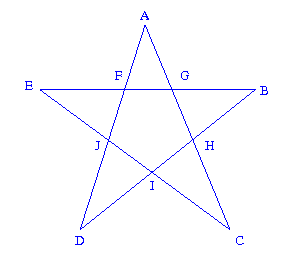
\includegraphics{figures/star}}

\vfill

}

\workbookpagebreak

\item Sketch a graph of the relation 
\[
\{ (x,y) \suchthat x,y \in \Reals \; \mbox{and} \; y > x^2 \}.
\]

\hint{Is this the region above or below the curve $y=x^2$?}

\wbvfill

\item A function $f(x)$ is said to be \index{invertible function} 
\emph{invertible} if there is another function $g(x)$ such that 
$g(f(x)) = x$ for all values of $x$.  (Usually, the inverse function,
$g(x)$ would be denoted $f^{-1}(x)$.)   Suppose a function is presented 
to you as a relation -- that is, you are just given a set of pairs.  
How can you distinguish whether the function represented by this list 
of input/output pairs is invertible?  How can you produce the inverse 
(as a set of ordered pairs)?
 
\hint{If $f$ sends $x$ to $y$, then we want $f^{-1}$ to send $y$ back to $x$.  So the inverse just has the pairs in $f$ reversed.  When is the inverse going to fail to be a function?}

\wbvfill

\workbookpagebreak

\item There is a relation known as ``has color'' which goes from the
set 
\[ F = \{orange, cherry, pumpkin, banana\} \]
to the set 
\[ C = \{orange, red, green, yellow\}. \]

\noindent  What pairs are in ``has color''?
   
\hint{Depending on your personal experience level with fruit there may be different answers.  Certainly
(orange, orange) will be one of the pairs, but (orange, green) happens too!}

\wbvfill

\end{enumerate}


%\newpage
%\renewcommand{\bibname}{References for chapter 1}
%\bibliographystyle{plain}
%\bibliography{main}

%% Emacs customization
%% 
%% Local Variables: ***
%% TeX-master: "GIAM-hw.tex" ***
%% comment-column:0 ***
%% comment-start: "%% "  ***
%% comment-end:"***" ***
%% End: ***


\chapter{Logic and quantifiers}
\label{ch:logic}

\section{Predicates and Logical Connectives}
\label{sec:pred}

\noindent{\large \bf Exercises --- \thesection\ }

\begin{enumerate}

\item Design a digital logic circuit (using and, or \& not gates) that 
implements an exclusive or.

\wbvfill

\hint{First, it's essential to know what is meant by the term "exclusive or". This is the interpretation that many people give to the word "or" -- where "X or Y" means either X is true or Y is true, but that it isn't the case that both X and Y are true. This (wrong) understanding of what "or" means is common because it is often the case that X and Y represent complimentary possibilities: old or new, cold or hot, right or wrong... The truth table for exclusive or (often written xor, pronounced "ex-or", symbolically it is usually $\oplus$) is

\begin{tabular}{|c|c|c|} \hline
\rule[-8pt]{0pt}{30pt}$X$ & $Y$ & $X \,\oplus\, Y$ \\ \hline
\rule[-8pt]{0pt}{30pt}$T$ & $T$ & $\phi$ \\ \hline
\rule[-8pt]{0pt}{30pt}$T$ & $\phi$ & $T$ \\ \hline
\rule[-8pt]{0pt}{30pt}$\phi$ & $T$ & $T$ \\ \hline
\rule[-8pt]{0pt}{30pt}$\phi$ & $\phi$ & $\phi$  \\ \hline
\end{tabular}

\noindent So it's true when one, or the other, but not both of its inputs are true.  The upshot of the last sentence is that we can write $X \oplus Y \; \equiv \; (X \lor Y) \land {\lnot}(X \land Y)$.

The above reformulation should help\ldots 

\vfill

}

\workbookpagebreak

\item Consider the sentence 
``This is a sentence which does not refer to itself.''
which was given in the beginning of this chapter as an example.
Is this sentence a statement?  If so, what is its truth value?

\hint{The only question in your mind, when deciding whether a sentence is a statement, should be "Does this thing have a definite truth value?"
Well?

Isn't it just plainly false?}

%\vspace{.5in}
\vfill

\item Consider the sentence ``This sentence is false.''  Is this 
sentence a statement?

\hint{Try to justify why this sentence can't be either true or false.}

\hintspagebreak

%\vspace{.5in}
\vfill

\workbookpagebreak

\item Complete truth tables for each of the sentences 
$(A \land B) \lor C$ and
$A \land (B \lor C)$.  Does it seem that these sentences have
the same logical content?

\hint{

\vfill

A tiny hint here: since the sentences involve 3 variables you'll need truth tables with 8 rows. Here's a template.

\vfill

\begin{tabular}{|c|c|c|c|c|} \hline
\rule[-8pt]{0pt}{30pt}$A$ & $B$ & $C$ & $(A \land B) \lor C$ & $A \land (B \lor C)$ \\ \hline
\rule[-8pt]{0pt}{30pt}$T$ & $T$ & $T$ & \rule{100pt}{0pt} & \rule{100pt}{0pt} \\ \hline
\rule[-8pt]{0pt}{30pt}$T$ & $T$ & $\phi$  & & \\ \hline
\rule[-8pt]{0pt}{30pt}$T$ & $\phi$  & $T$ & & \\ \hline
\rule[-8pt]{0pt}{30pt}$T$ & $\phi$  & $\phi$  & & \\  \hline
\rule[-8pt]{0pt}{30pt}$\phi$  & $T$ & $T$ & & \\ \hline
\rule[-8pt]{0pt}{30pt}$\phi$  & $T$ & $\phi$  & & \\ \hline
\rule[-8pt]{0pt}{30pt}$\phi$  & $\phi$  & $T$ & & \\ \hline
\rule[-8pt]{0pt}{30pt}$\phi$  & $\phi$  & $\phi$  & & \\  \hline
\end{tabular}
}
\vfill

\hintspagebreak
\workbookpagebreak

\item \label{ex:nand_nor} There are two other logical connectives that are
used somewhat less commonly than $\lor$ and $\land$.
These are the \index{Scheffer stroke} Scheffer stroke and the 
\index{Peirce arrow}Peirce arrow
-- written $\vert$ and $\downarrow$, respectively ---  they are 
also known as \index{NAND} NAND and \index{NOR} NOR.

\noindent The truth tables for these connectives are:
\medskip

\begin{tabular}{c|c|c}
$A$ & $B$ & $A \,\vert\, B$ \\ \hline
$T$ & $T$ & $\phi$ \\
$T$ & $\phi$ & $T$ \\
$\phi$ & $T$ & $T$ \\
$\phi$ & $\phi$ & $T$ 
\end{tabular}
\hspace{.25 in} and \hspace{.25 in}
\begin{tabular}{c|c|c}
$A$ & $B$ & $A \downarrow B$ \\ \hline
$T$ & $T$ & $\phi$ \\
$T$ & $\phi$ & $\phi$ \\
$\phi$ & $T$ & $\phi$ \\
$\phi$ & $\phi$ & $T$ 
\end{tabular}
\medskip

Find an expression for $(A\, \land {\lnot}B) \lor C$
using only these new connectives (as well as negation and the
variable symbols themselves).


\hint{Sorry, I know this is probably the hardest problem in the chapter, but I'm (mostly) not going to help...
Just one hint to help you get started: NAND and NOR are the negations of AND and OR (respectively) so, for example, $(X \land Y) \; \equiv \; {\lnot}(A \,\vert\, B)$.}

\textbookpagebreak
\workbookpagebreak


\item \label{IKK} The famous logician \index{Smullyan, Raymond} Raymond Smullyan devised 
a family of logical puzzles around a fictitious place he called 
\index{Knights and Knaves} ``the Island of Knights and Knaves.''  The inhabitants of the island are either knaves, who always make false statements, or knights, who always make truthful statements.  

In the most famous knight/knave puzzle, you are in a room which has only two exits.  One leads to certain death and the other to freedom.  There are two 
individuals in the room, and you know that one of them is a knight and the other is a knave, but you don't know which.   Your challenge is to determine the door which leads to freedom by asking a single question.

\hint{Ask one of them what the other one would say to do.}

\end{enumerate}


\newpage

\section{Implication}
\label{sec:impl}

\noindent{\large \bf Exercises --- \thesection\ }

\begin{enumerate}

\item The transitive property of equality says that if $a=b$ and $b=c$
then $a=c$.  Does the implication arrow satisfy a transitive property?
If so, state it.

\wbvfill

\hint{
I sometimes like to rephrase the implication $X \implies Y$ as ``X's truth forces Y to be true.''  Does that help?
If we know that X being true forces Y to be true, and we also know that Y being true will force Z to be true, what can we conclude?

\vfill

}

\item Complete truth tables for the compound sentences $A \implies B$ and
  ${\lnot}A \lor B$.
  
  \wbvfill
  
\hint{
You should definitely be able to do this one on your own, but anyway, here's an outline of the table:

\begin{tabular}{|c|c|c|c|} \hline
\rule[-6pt]{0pt}{24pt}  $A$ & $B$ & $A \implies B$ & ${\lnot}A \lor B$ \\ \hline
\rule[-6pt]{0pt}{24pt}  $T$ &  $T$ & & \\ \hline
\rule[-6pt]{0pt}{24pt}  $T$ & $\phi$ & & \\ \hline	 	 
\rule[-6pt]{0pt}{24pt}  $\phi$ & $T$ & & \\ \hline
\rule[-6pt]{0pt}{24pt}  $\phi$ & $\phi$ & & \\ \hline
\end{tabular}

\vfill

}

\item Complete a truth table for the compound sentence $A \implies (B \implies C)$ and for the sentence $(A \implies B) \implies C$.  What can you conclude
about conditionals and the associative property?

\wbvfill

\hint{
No help on this one other than to say that the associative property {\bf does not} hold for implications.

\vfill

}

\workbookpagebreak
\hintspagebreak

\item Determine a sentence using the {\em and} connector ($\land$) that
gives the negation of $A \implies B$.

\wbvfill

\hint{Hmmm\ldots This will seem like a strange hint, but if you were to hear a kid at the playground say ``Oh yeah? Well, I did call your mom a fatty and you still haven't clobbered me! Owww! OWWW!!! Stop hitting me!!''

What conditional sentence was he attempting to negate?
}

\item Rewrite the sentence ``Fix the toilet or I won't pay the rent!'' as
a conditional.

\wbvfill

\hint{The way I see it there are eight possible ways to arrange "You fix the toilet" and "I'll pay the rent" (or their respective negations) around an implication arrow.
Here they all are. You decide which one sounds best.

If you fix the toilet, then I'll pay the rent.\newline
If you fix the toilet, then I won't pay the rent.\newline
If you don't fix the toilet, I'll pay the rent.\newline
If you don't fix the toilet, then I won't pay the rent.\newline
If I payed the rent, then you must have fixed the toilet.\newline
If I payed the rent, then you must not have fixed the toilet.\newline
If I didn't pay the rent, then you must have fixed the toilet.\newline
If I didn't pay the rent, then you must not have fixed the toilet.\newline

Some of those are truly strange\ldots
}
\item Why is it that the sentence ``If pigs can fly, I am the king
of Mesopotamia.'' true?

\wbvfill

\hint{Unless we're talking about some celebrity bringing their pet Vietnamese pot-bellied pig into first class with them, or possibly a catapult of some type... The antecedent (the if part) is false, so Yay! I AM the king of Mesopotamia!! Whoo-hooh! What? I'm not? Oh. But the if-then sentence is true. Bummer.}

\item Express the statement $A \implies B$ using the Peirce arrow and/or the
Scheffer stroke. (See Exercise~\ref{ex:nand_nor} in the previous section.)

\wbvfill

\hint{You'll want to use $\vert$, the Scheffer stroke, aka NAND, because it's truth table contains three $T$'s and one $\phi$ -- you'll just need to figure out which of its inputs to negate so as to make that one $\phi$ occur in the second row of the table instead of the first.}

\workbookpagebreak

\item Find the contrapositives of the following sentences.
  \begin{enumerate}
  \item If you can't do the time, don't do the crime.
  \item If you do well in school, you'll get a good job.
  \item If you wish others to treat you in a certain way, you must 
    treat others in that fashion.
  \item If it's raining, there must be clouds.
  \item If $a_n \leq b_n$, for all $n$ and $\sum_{n=0}^\infty b_n$ is a 
convergent series, then $\sum_{n=0}^\infty a_n$ is a convergent series.
  \end{enumerate}

\wbvfill

\hint{
\begin{enumerate}
\item If you do the crime, you must do the time.
\item If you don't have a good job, you must've done poorly in school.
\item If you don't treat others in a certain way, you can't hope for others to treat you in that fashion,
\item If there are no clouds, it can't be raining.
\item If  $\sum_{n=0}^\infty a_n$ is not a convergent series, then either $a_n \leq b_n$, for some $n$ or 
$\sum_{n=0}^\infty b_n$ is not a convergent series.
\end{enumerate}
}
\rule{0pt}{0pt}

\wbvfill

\item What are the converse and inverse of ``If you watch my back, I'll 
watch your back.''?

\wbvfill

\hint{
The converse is ``If I watch your back, then you'll watch my back.''  (Sounds a little dopey doesn't it -- likes its sort of a wishful thinking\ldots)
The inverse is ``If you don't watch my back, then I won't watch your back.''  (Sounds less vapid, but it means the same thing\ldots)
}

\workbookpagebreak

\item The integral test in Calculus is used to determine whether an
infinite series converges or diverges:   Suppose that $f(x)$ is a positive,
decreasing, 
real-valued function with $\lim_{x \longrightarrow \infty} f(x) = 0$, if
the improper integral
$\int_0^\infty f(x)$ has a finite value, then the infinite series 
$\sum_{n=1}^\infty f(n)$ converges.

The integral test should be envisioned by letting the series correspond
to a right-hand Riemann sum for the integral, since the function is decreasing,
a right-hand Riemann sum is an underestimate for the value of the integral,
thus

\[ \sum_{n=1}^\infty f(n) < \int_0^\infty f(x). \]

Discuss the meanings of and (where possible) provide justifications for
the inverse, converse and contrapositive of the conditional statement 
in the integral test.

\wbvfill

\hint{
The inverse says -- if the integral isn't finite, then the series doesn't converge. You can cook-up a function that shows this to be false by (for example) creating one with vertical asymptotes that occur in between the integer $x$-values. Even one such pole can be enough to make the integral go infinite.
The converse says that if the series converges, the integral must be finite. The counter-example we just discussed would work here too.

The contrapositive says that if the series doesn't converge, then the integral must not be finite. If we were allowed to use discontinuous functions, it isn't too hard to come up with an $f$ that actually has zero area under it -- just make f be identically zero except at the integer x-values where it will take the same values as the terms of the series. But wait, the function we just described isn't ``decreasing'' -- which is probably why that hypothesis was put in there!
}

\workbookpagebreak

\item On the Island of Knights and Knaves (see page~\pageref{IKK}) you encounter two individuals named Locke and Demosthenes.  

Locke says, ``Demosthenes is a knave.'' \newline
Demosthenes says ``Locke and I are knights.''

Who is a knight and who a knave?

\wbvfill

\hint{Could Demosthenes be telling the truth?}

\end{enumerate}


\newpage

\section{Logical equivalences}
\label{sec:le}

\noindent{\large \bf Exercises --- \thesection\ }

\begin{enumerate}

\item There are 3 operations used in basic algebra (addition, 
multiplication and exponentiation) and thus
there are potentially 6 different distributive laws.  State
all 6 ``laws'' and determine which 2 are actually valid.
(As an example, the distributive law of addition over multiplication
would look like $x + (y \cdot z) = (x + y) \cdot (x + z)$, this isn't 
one of the true ones.) 

\wbvfill

\hint{
\vfill

These ``laws'' should probably be layed-out in a big 3 by 3 table. Such a table would of course have 9 cells, but we won't be using the cells on the diagonal because they would involve an operation distributing over itself. (That can't happen, can it?)
I'm going to put a few of the entries in, and you do the rest.

\vfill

\begin{tabular}{c|c|c|c|} 
  & \rule{36pt}{0pt} $+$ \rule{36pt}{0pt} & \rule{36pt}{0pt} $\ast$ \rule{36pt}{0pt} & \rule{36pt}{0pt} $\caret$ \rule{36pt}{0pt} \\ \hline
 \rule[-36pt]{0pt}{72pt} $+$ & $\emptyset$ & \parbox{1.4in}{\begin{gather*}x+(y\ast z) \\= (x+y) \ast (x+z)\end{gather*}} & \parbox{1.4in}{\begin{gather*}x+(y^z) \\ = (x+y)^{(x+z)} \end{gather*} } \\ \hline
 \rule[-36pt]{0pt}{72pt} $\ast$ & \parbox{1.4in}{\begin{gather*} x \ast (y+z) \\ = (x \ast y) + (x \ast z)\end{gather*} } & $\emptyset$ &  \\ \hline
 \rule[-36pt]{0pt}{72pt} $\caret$ & & & $\emptyset$ \\ \hline
\end{tabular}

\vfill

\rule{0pt}{0pt}
 }
 
 \workbookpagebreak
\hintspagebreak
 
\item Use truth tables to verify or disprove the following 
logical equivalences.

\begin{enumerate}
\item $(A \land B) \lor B \; \cong \; (A \lor B) \land B$
\item $A \land (B \lor {\lnot}A) \; \cong \; A \land B $
\item $(A \land {\lnot}B) \lor ({\lnot}A \land {\lnot}B) \cong
(A \lor {\lnot}B) \land ({\lnot}A \lor {\lnot}B)$ 
\item The absorption laws.
\end{enumerate}

\wbvfill

\hint{You should be able to do these on your own.}

\workbookpagebreak

\item Draw pairs of related digital logic circuits that illustrate
DeMorgan's laws.

\wbvfill

\hint{
Here's the pair that shows the negation of an AND is the same as the OR of the same inputs negated.

\centerline{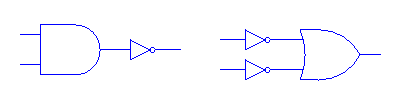
\includegraphics{figures/DeMorgan}}
}

\item Find the negation of each of the following and simplify as much as possible.
\medskip

  \begin{enumerate}
  \item $(A \lor B) \; \iff \; C$
\medskip

  \item $(A \lor B) \; \implies \; (A \land B)$

  \end{enumerate}

\wbvfill

\hint{Neither of these is particularly amenable to simplification. Nor, perhaps, is it readily
apparent what ``simplify'' means in this context! My interpretation is that we should look
for a logically equivalent expression using the fewest number of operators and if possible
{\em not} using the more complicated operators ($\implies$ and $\iff$).  However, if we try 
to rewrite the first statement's negation using only $\land$, $\lor$ and $\lnot$ we get things
that look a lot more complicated than $(A \lor B) \; \iff \; {\lnot}C$ -- the quick way to negate a 
bicondiitonal is simply to negate one of its parts.

The second statement's negation turns out to be the same thing as exclusive or, so a particularly
simple response would be to write $A \oplus B$ although that feels a bit like cheating, so
maybe we should answer with $(A \lor B) \land {\lnot}(A \land B)$ -- but that answer is what we
would get by simply applying the rule for negating a conditional and doing no further simplification.
}

\workbookpagebreak

\item Because a conditional sentence is equivalent to a certain disjunction, and 
because DeMorgan's law tells us that the negation of a disjunction is a conjunction,
it follows that the negation of a conditional is a conjunction.  Find denials (the negation
of a sentence is often called its ``denial'') for each of the following conditionals.

\begin{enumerate}
\item ``If you smoke, you'll get lung cancer.''
\item ``If a substance glitters, it is not necessarily gold.''
\item ``If there is smoke, there must also be fire.''
\item ``If a number is squared, the result is positive.''
\item ``If a matrix is square, it is invertible.''
\end{enumerate}

\wbvfill

\hint{
\begin{enumerate}
\item ``You smoke and you haven't got lung cancer.''
\item ``A substance glitters and it is necessarily gold.''
\item ``There is smoke,and there isn't fire.''
\item ``A number is squared, and the result is not positive.''
\item ``A matrix is square and it is not invertible.''
\end{enumerate}
}

\hintspagebreak
\workbookpagebreak

\item The so-called ``ethic of reciprocity'' is an idea that has come 
up in many of the world's religions and philosophies.  
Below are statements of the ethic
from several sources.  Discuss their logical meanings and determine which (if 
any) are logically equivalent.

\begin{enumerate}
\item ``One should not behave towards others in a way which is disagreeable to oneself.'' Mencius Vii.A.4 (Hinduism)
\item ``None of you [truly] believes until he wishes for his brother what he wishes for himself.'' Number 13 of Imam ``Al-Nawawi's Forty Hadiths.'' (Islam)
\item ``And as ye would that men should do to you, do ye also to them likewise.'' Luke 6:31, King James Version. (Christianity)
\item ``What is hateful to you, do not to your fellow man. This is the law: all the rest is commentary.'' Talmud, Shabbat 31a. (Judaism)
\item ``An it harm no one, do what thou wilt'' (Wicca)
\item ``What you would avoid suffering yourself, seek not to impose on others.'' (the Greek philosopher Epictetus -- first century A.D.)
\item ``Do not do unto others as you expect they should do unto you. Their tastes may not be the same.'' (the Irish playwright George Bernard Shaw -- 20th century A.D.)
\end{enumerate}

\wbvfill

\hint{
The ones from Wicca and George Bernard Shaw are just there for laughs.

For the remainder, you may want to contrast how restrictive they seem. For example the Christian version is (in my opinion) a lot stronger than the one from the Talmud -- ``treat others as you would want to be treated'' restricts your actions both in terms of what you would like done to you and in terms of what you wouldn't like done to you; ``Don't treat your fellows in a way that would be hateful to you.'' is leaving you a lot more freedom of action, since it only prohibits you from doing those things you wouldn't want done to yourself to others. The Hindus, Epictetus and the Jews (and the Wiccans for that matter) seem to be expressing roughly the same sentiment -- and promoting an ethic that is rather more easy for humans to conform to!

From a logical perspective it might be nice to define open sentences:

\[ W(x,y) \; = \; \mbox{``x would want y done to him.''} \]

\[ N(x,y)  \; = \; \mbox{``x would not want y done to him.''} \]

\[ D(x,y)  \; = \; \mbox{``do y to x.''} \]

\[ DD(x,y)  \; = \; \mbox{``don't do y to x.''} \]

In which case, the aphorism from Luke would be

\[ (W(you, y) \implies  D(others, y)) \land (N(you, y) \implies DD(others, y)) \]

}

\workbookpagebreak
\textbookpagebreak

\item You encounter two natives of the land of knights and knaves. Fill
in an explanation for each line of the proofs of their identities. 

\begin{enumerate}
\item Natasha says, ``Boris is a knave.'' \\
Boris says, ``Natasha and I are knights.''\\

\hintspagebreak

\textbf{Claim:} Natasha is a knight, and Boris is a knave.\\

\begin{proof} If Natasha is a knave, then Boris is a knight.\\
If Boris is a knight, then Natasha is a knight.\\
Therefore, if Natasha is a knave, then Natasha is a knight.\\
Hence Natasha is a knight.\\
Therefore, Boris is a knave.
\end{proof}

\item Bonaparte says ``I am a knight and Wellington is a knave.''\\
Wellington says ``I would tell you that B is a knight.''

\textbf{Claim:} Bonaparte is a knight and Wellington is a knave.

\begin{proof}
    Either Wellington is a knave or Wellington is a knight.\\
    If Wellington is a knight it follows that Bonaparte is a knight.\\
    If Bonaparte is a knight then Wellington is a knave. \\
    So, if Wellington is a knight then Wellington is a knave (which is impossible!)\\
    Thus, Wellington is a knave.\\
    Since Wellington is a knave, his statement ``I would tell you that Bonaparte is a knight'' is false. \\
    So Wellington would in fact tell us that Bonaparte is a knave. \\
    Since Wellington is a knave we conclude that Bonaparte is a knight.\\
    Thus Bonaparte is a knight and Wellington is a knave (as claimed).\\
\end{proof}

\hintspagebreak
\wbvfill

\hint{
Here's the second one:

\begin{proof}
    Either Wellington is a knave or Wellington is a knight.\\
    \rule{0pt}{0pt} \hfill \parbox{3in}{\color[rgb]{1,0,0} It's either one thing or the other! }\\
    If Wellington is a knight it follows that Bonaparte is a knight.\\
    \rule{0pt}{0pt} \hfill \parbox{3in}{\color[rgb]{1,0,0} That's what he said he would tell us and if he's a knight we can trust him.}\\
    If Bonaparte is a knight then Wellington is a knave. \\
    \rule{0pt}{0pt} \hfill \parbox{3in}{\color[rgb]{1,0,0} True, because that is one of the things Bonaparte states.}\\
    So, if Wellington is a knight then Wellington is a knave (which is impossible!)\\
    \rule{0pt}{0pt} \hfill \parbox{3in}{\color[rgb]{1,0,0} This is just summing up what was deduced above.}\\
    Thus, Wellington is a knave.\\
    \rule{0pt}{0pt} \hfill \parbox{3in}{\color[rgb]{1,0,0}  Because the other possibility leads to something {\em im}possible.}\\
    Since Wellington is a knave, his statement ``I would tell you that Bonaparte is a knight'' is false. \\
    \rule{0pt}{0pt} \hfill \parbox{3in}{\color[rgb]{1,0,0} Knave's statements are always false!}\\
    So Wellington would in fact tell us that Bonaparte is a knave. \\
    \rule{0pt}{0pt} \hfill \parbox{3in}{\color[rgb]{1,0,0} He was lying when he said he would tell us B is a knight.} \\
    Since Wellington is a knave we conclude that Bonaparte is a knight.\\
    \rule{0pt}{0pt} \hfill \parbox{3in}{\color[rgb]{1,0,0} Wait, now I'm confused\ldots can you do this part?} \\
    Thus Bonaparte is a knight and Wellington is a knave (as claimed).\\
    \rule{0pt}{0pt} \hfill \parbox{3in}{\color[rgb]{1,0,0} Just summarizing.} \\
\end{proof}

}

\end{enumerate}

\end{enumerate}


\newpage
\section{Two-column proofs}
\label{sec:2_col}

\noindent{\large \bf Exercises --- \thesection\ }

Write two-column proofs that verify each of the following
logical equivalences.

\begin{enumerate}
\item $A \lor (A \land B) \; \cong \; A \land (A \lor B)$
\medskip

\item $(A \land {\lnot}B) \lor A \; \cong \; A$
\medskip

\item $A \lor B \; \cong \; A \lor ({\lnot}A \land B)$
\medskip

\item ${\lnot}(A \lor {\lnot}B) \lor ({\lnot}A \land {\lnot}B) \; \cong \; {\lnot}A$
\medskip

\item $A \; \cong \; A \land ((A \lor {\lnot}B) \lor (A \lor B))$
\medskip

\item $(A \land {\lnot}B) \land ({\lnot}A \lor B) \; \cong \; c$
\medskip

\item $A \; \cong \; A \land (A \lor (A \land (B \lor C)))$
\medskip

\item ${\lnot}(A \land B) \land {\lnot}(A \land C) \; \cong \; {\lnot}A \lor ({\lnot}B \land {\lnot}C)$
\medskip

\end{enumerate}

\hint{
Here's the last one:

\begin{proof}

$  {\lnot}(A \land B) \land {\lnot}(A \land C) $ \\  
 \rule{0pt}{0pt} \hfill \parbox{3in}{\color[rgb]{1,0,0}  	 DeMorgan's law (times 2)} \\
$\equiv  \quad   ({\lnot}A \lor {\lnot}B) \land ({\lnot}A \lor {\lnot}C)	$ \\   
 \rule{0pt}{0pt} \hfill \parbox{3in}{\color[rgb]{1,0,0}  	 Distributive law} \\ 
$\equiv  \quad  {\lnot}A \lor ({\lnot}B \land {\lnot}C) $ \\  
\end{proof}

}
\workbookpagebreak

\rule{0pt}{0pt}

\workbookpagebreak

\newpage

\section{Quantified statements}
\label{sec:quant}

\noindent{\large \bf Exercises --- \thesection\ }

\begin{enumerate}
\item There is a common variant of the existential quantifier,
$\exists !$, if you write $\exists ! \, x, \, P(x)$ you are asserting 
that there is a \index{unique existence}\emph{unique} element 
in the universe that makes $P(x)$ true.
Determine how to negate the sentence $\exists ! \, x, \, P(x)$.

\hint{
Unique existence is essentially saying that there is exactly 1 element of the universe of discourse that makes P(x) true. The negation of "there is exactly 1" is "there's either none, or at least 2".

Is that enough of a hint?
}

\item The order in which quantifiers appear is important.  Let $L(x,y)$
be the open sentence ``$x$ is in love with $y$.''  Discuss the meanings of the
following quantified statements and find their negations.

\begin{enumerate}
\item $\forall x \, \exists y \; L(x,y)$.
\item $\exists x \, \forall y \; L(x, y)$.
\item $\forall x \, \forall y \; L(x, y)$.
\item $\exists x \, \exists y \; L(x, y)$.
\end{enumerate}

\hint{

\begin{enumerate}
\item $\forall x \, \exists y \; L(x,y)$.

This is a fairly optimistic statement  ``For everyone out there, there's somebody that they are in love with.''

\item $\exists x \, \forall y \; L(x, y)$.

This one, on the other hand, says something fairly strange: ``There's someone who has fallen in love with every other human being.'' I don't know, maybe the Dalai Lama? Mother Theresa?...
Anyway, do the last two for yourself.

\item $\forall x \, \forall y \; L(x, y)$.
\item $\exists x \, \exists y \; L(x, y)$.

\vspace{.5in}

Here's a couple of bonus questions. Two of the statements above have different meanings if you just interchange the order that the quantifiers appear in. What do the following mean (in contrast to the ones above)?

\item $\exists y \, \forall x \; L(x, y)$.
\item $\forall y \, \exists x \; L(x,y)$.
\end{enumerate}

}

\item Determine a useful denial of: 

$\displaystyle \forall \epsilon>0 \, \exists 
\delta>0 \, \forall x \, (|x-c| < \delta) \implies (|f(x)-l| < \epsilon) $.

The denial above gives a criterion for saying $\lim_{x\rightarrow c}f(x) \neq l.$

\hint{
This is asking you to put a couple of things together. The first thing is that in negating a quantified statement, we get a new statement with all the quantified variables occurring in the same order but with $\forall$'s and $\exists$'s interchanged. The second issue is that the logical statement that appears after all the quantifiers needs to be negated. Since, in this statement we have a conditional, you must remember to negate that properly (its negation is a conjunction).

$\displaystyle \exists \epsilon>0 \, \forall 
\delta>0 \, \exists x \, (|x-c| < \delta)  \land  (|f(x)-l| \geq \epsilon) $.

}

\item A \index{Sophie Germain prime} \emph{Sophie Germain prime} is a prime number $p$
such that the corresponding odd number $2p+1$ is also a prime.  For example 11 is a 
Sophie Germain prime since $23 = 2\cdot 11 + 1$ is also prime.  Almost all Sophie Germain
primes are congruent to $5 \pmod{6}$, nevertheless, there are exceptions -- so the
statement ``There are Sophie Germain primes that are not 5 mod 6.'' is true.  Verify this.

\hint{The exceptions are very small prime numbers. You should be able to find them easily.}

\item  Alvin, Betty, and Charlie enter a cafeteria which offers three different
entrees, turkey sandwich, veggie burger, and pizza; four different
beverages, soda, water, coffee, and milk; and two types of desserts,
pie and pudding. Alvin takes a turkey sandwich, a soda, and a pie.
Betty takes a veggie burger, a soda, and a pie. Charlie takes a pizza
and a soda. Based on this information, determine whether the following
statements are true or false.

\begin{enumerate}
\item \label{negated}$\forall$ people $p$, $\exists$ dessert $d$ such that $ p$
took $d$. \hint{false}
\item \label{compare}$\exists$ person $p$ such that $\forall$ desserts
$d$, $p$ did not take $d$. \hint{true}
\item $\forall$ entrees $e$, $\exists$ person $p$ such that $ p$ took
$e$. \hint{true}
\item \label{entree}$\exists$ entree $e$ such that  $\forall$ people
$p,\ p$ took $e$. \hint{false}
\item $\forall$ people $p$, $p$ took a dessert $\iff p$ did not take
a pizza. \hint{true}
\item Change one word of statement \ref{entree} so that it becomes true. \hint{entree $\longrightarrow$ beverage}
\item Write down the negation of \ref{negated} and compare it to statement
\ref{compare}. Hopefully you will see that they are the same! Does
this make you want to modify one or both of your answers to \ref{negated}
and \ref{compare}? \hint{$\exists$ person $p$ such that $\forall$ desserts
$d$, $p$ did not take $d$. Yes I do.  No, I got them right in the first place!}
\end{enumerate}

\end{enumerate}


\newpage

\section{Deductive reasoning and Argument forms}
\label{sec:deduct}

\noindent{\large \bf Exercises --- \thesection\ }

\begin{enumerate}

\item In the movie ``Monty Python and the Holy Grail'' we encounter
a medieval villager who (with a bit of prompting) makes the 
following argument.

\begin{quote}
If she weighs the same as a duck, then she's made of wood. \newline
If she's made of wood then she's a witch. \newline
Therefore, if she weighs the same as a duck, she's a witch.
\end{quote} 

Which rule of inference is he using?

\hint{
This is what many people refer to as the transitive rule of implication.  As an argument form it's known as ``hypothetical syllogism.''
}

\item In constructive dilemma, the antecedent of the conditional 
sentences are usually chosen to represent opposite alternatives. 
This allows us to introduce their disjunction as a tautology. 
Consider the following proof that there is never any reason to worry
(found on the walls of an Irish pub).

\begin{quote}
Either you are sick or you are well. \newline
If you are well there's nothing to worry about. \newline
If you are sick there are just two possibilities: \newline
Either you will get better or you will die. \newline
If you are going to get better there's nothing to worry about. \newline
If you are going to die there are just two possibilities:\newline
Either you will go to Heaven or to Hell. \newline
If you go to Heaven there is nothing to worry about.
If you go to Hell, you'll be so busy shaking hands with all your friends there won't be time to worry \ldots
\end{quote}

Identify the three tautologies that are introduced in this ``proof.''

\hint{Look at the lines that start with the word "Either."}

\textbookpagebreak

\item For each of the following arguments, write it in symbolic form and determine 
which rules of inference are used.

\begin{enumerate}
\item \rule{0pt}{24pt} You are either with us, or you're against us.  And you don't appear to be with us.
So, that means you're against us!

\hint{
\begin{center}
\begin{tabular}{cl}
 & $W \lor A$ \\
 & ${\lnot}W$ \\ \hline
$\therefore$ & $A$ \\
\end{tabular}
\end{center}

This is ``disjunctive syllogism.''
}


\item \rule{0pt}{24pt} All those who had cars escaped the flooding.  Sandra had a car -- therefore, Sandra
escaped the flooding.

\hint{
Let $C(x)$ be the open sentence ``x has a car'' and let $E(x)$ be the open sentence ``x escaped the flooding.''
This argument is actually the particular form of universal modus ponens: (See the final question in the next set of exercises.)

\begin{center}
\begin{tabular}{cl}
 & $\forall x, C(x) \implies E(x)$ \\
 & $C(\mbox{Sandra}) $ \\ \hline
$\therefore$ & $E(\mbox{Sandra})$ \\
\end{tabular}
\end{center}

At this stage in the game it would be perfectly fine to just identify this as modus ponens and not worry about the quantifiers that appear.
}

\item \rule{0pt}{24pt}  When Johnny goes to the casino, he always gambles 'til he goes broke.  Today, Johnny
has money, so Johnny hasn't been to the casino recently.
\item \rule{0pt}{24pt} (A non-constructive proof that there are 
irrational numbers $a$ and $b$ such that $a^b$ is rational.)  
Either $\sqrt{2}^{\sqrt{2}}$ is rational or it is irrational.
If $\sqrt{2}^{\sqrt{2}}$ is rational, we let $a=b=\sqrt{2}$.
Otherwise, we let $a=\sqrt{2}^{\sqrt{2}}$ and $b=\sqrt{2}$.
(Since $\sqrt{2}^{\sqrt{2}^{\sqrt{2}}} = 2$, which is rational.) It follows that in either case, there
are irrational numbers $a$ and $b$ such that $a^b$ is rational.


\end{enumerate}

\hint{I'm leaving the last two for you to do. One small hint: both are valid forms.}


\end{enumerate}


\newpage

\section{Validity of arguments and common errors}
\label{sec:valid}

\noindent{\large \bf Exercises --- \thesection\ }

\begin{enumerate}
\item Determine the logical form of the following arguments.  Use symbols
to express that form and determine whether the form is valid or invalid.
If the form is invalid, determine the type of error made.  Comment on the 
soundness of the argument as well, in particular, determine whether any of
the premises are questionable.
\begin{enumerate}
\item All who are guilty are in prison. \newline
  George is not in prison.  \newline
  Therefore, George is not guilty.
 
  \hint{ 
  This looks like modus tollens. Let $G$ refer to ``guilt'' and $P$ refer to ``in prison''
  
\begin{center}
\begin{tabular}{cl}
 & $\forall x, G(x) \implies P(x)$ \\
 & ${\lnot}P(\mbox{George}) $ \\ \hline
$\therefore$ & ${\lnot}G(\mbox{George})$ \\
\end{tabular}
\end{center}

You should note that while the form is valid, there is something terribly wrong with this argument. Is it really true that everyone who is guilty of a crime is in prison?
}

\item If one eats oranges one will have high levels of vitamin C. \newline
  You do have high levels of vitamin C. \newline
  Therefore, you must eat oranges.
\item All fish live in water. \newline
  The mackerel is a fish. \newline
  Therefore, the mackerel lives in water. 
\item If you're lazy, don't take math courses.\newline
  Everyone is lazy. \newline
  Therefore, no one should take math courses.
\item All fish live in water. \newline
  The octopus lives in water. \newline
  Therefore, the octopus is a fish.
\item If a person goes into politics, they are a scoundrel.\newline
  Harold has gone into politics. \newline
  Therefore, Harold is a scoundrel. 
\end{enumerate}

\item Below is a rule of inference that we call extended elimination.

\begin{tabular}{cl}
 & $(A \lor B) \lor C$ \\
 & ${\lnot}A$ \\
 & ${\lnot}B$ \\ \hline
$\therefore$ & $C$ \\
\end{tabular}

Use a truth table to verify that this rule is valid.

\hint{

\vfill

In the following truth table the predicate variables occupy the first 3 columns, the argument's 
premises are in the next three columns and the conclusion is in the right-most column.  The
truth values have already been filled-in.  You only need to identify the critical rows and 
verify that the conclusion is true in those rows.

\vfill

 \newpage
 
\begin{tabular}{|c|c|c||c|c|c||c|} \hline
\rule[-8pt]{0pt}{30pt}$A$ & $B$ & $C$ & $(A \lor B) \lor C$ & \rule{20pt}{0pt} ${\lnot}A$ \rule{20pt}{0pt} & \rule{20pt}{0pt} ${\lnot}B$ \rule{20pt}{0pt} & \rule{20pt}{0pt} $C$ \rule{20pt}{0pt} \\ \hline
\rule[-8pt]{0pt}{30pt}$T$ & $T$ & $T$ & $T$ & $\phi$ & $\phi$ & $T$  \\ \hline
\rule[-8pt]{0pt}{30pt}$T$ & $T$ & $\phi$  & $T$ & $\phi$ & $\phi$ & $\phi$   \\ \hline
\rule[-8pt]{0pt}{30pt}$T$ & $\phi$  & $T$ & $T$ & $\phi$ & $T$  & $T$  \\ \hline
\rule[-8pt]{0pt}{30pt}$T$ & $\phi$  & $\phi$  & $T$ & $\phi$ & $T$ & $\phi$   \\  \hline
\rule[-8pt]{0pt}{30pt}$\phi$  & $T$ & $T$ & $T$ & $T$ & $\phi$ &  $T$ \\ \hline
\rule[-8pt]{0pt}{30pt}$\phi$  & $T$ & $\phi$  & $T$ & $T$ & $\phi$ & $\phi$  \\ \hline
\rule[-8pt]{0pt}{30pt}$\phi$  & $\phi$  & $T$ & $T$ & $T$ & $T$ & $T$  \\ \hline
\rule[-8pt]{0pt}{30pt}$\phi$  & $\phi$  & $\phi$  & $\phi$ & $T$ & $T$ & $\phi$  \\  \hline
\end{tabular}

\vfill
}

\item If we allow quantifiers and open sentences in an argument form we
get a couple of new argument forms.  Arguments involving existentially quantified 
premises are rare -- the new forms we are speaking of are called ``universal modus 
ponens'' and ``universal modus tollens.''   The minor premises may also be quantified
or they may involve particular elements of the universe of discourse -- this leads
us to distinguish argument subtypes that are termed ``universal'' and ``particular.''

For example  \begin{tabular}{cl}
 & $\forall x, A(x) \implies B(x)$ \\
 & $A(p)$ \\ \hline
$\therefore$ & $B(p)$ \\
\end{tabular}  is the particular form of universal modus ponens (here, $p$
is not a variable -- it stands for some particular element of the universe of
discourse)
and \begin{tabular}{cl}
 & $\forall x, A(x) \implies B(x)$ \\
 & $\forall x, {\lnot}B(x)$ \\ \hline
$\therefore$ & $\forall x, {\lnot}A(x)$ \\
\end{tabular} is the universal form of (universal) modus tollens.

Reexamine the arguments from problem (1), determine their forms
(including quantifiers) and whether they are universal or particular.

\hint{
Hint: All of them except for one are the particular form -- number 4 is the exception.

Here's an analysis of number 5:

All fish live in water. \newline
The octopus lives in water.  \newline
Therefore, the octopus is a fish. \newline

Let $F(x)$ be the open sentence ``x is a fish'' and let $W(x)$ be the open sentence ``x lives in water.''

Our argument has the form

 \begin{center}
\begin{tabular}{cl}
 & $\forall x, F(x) \implies W(x)$ \\
 & $W(\mbox{the octopus}) $ \\ \hline
$\therefore$ & $F(\mbox{the octopus})$ \\
\end{tabular}
\end{center}

Clearly something is wrong -- a converse error has been made -- if everything that lived in water was necessarily a fish the argument would be OK (in fact it would then be the particular form of universal modus ponens).  But that is the converse of the major premise given.    
}

\item Identify the rule of inference being used.

\begin{enumerate}
\item The Buley Library is very tall.\\
Therefore, either the Buley Library is very tall or it has many
levels underground.

\hint{disjunctive addition}

\item The grass is green.\\
The sky is blue.\\
Therefore, the grass is green and the sky is blue.

\hint{conjunctive addition}

\item $g$ has order 3 or it has order 4.\\
If $g$ has order 3, then $g$ has an inverse.\\
If $g$ has order 4, then $g$ has an inverse.\\
Therefore, $g$ has an inverse.

\hint{constructive dilemma}

\item $x$ is greater than 5 and $x$ is less than 53.\\
Therefore, $x$ is less than 53.

\hint{conjunctive simplification}

\item If $a|b$, then $a$ is a perfect square.\\
If $a|b$, then $b$ is a perfect square.\\
Therefore, if $a|b$, then $a$ is a perfect square and $b$ is
a perfect square.

\hint{Note that the conclusion could be re-expressed as the conjunction of the two conditionals that
are found in the premises.  This is conjunctive addition with a bit of ``window dressing.''}
\end{enumerate}

\item Read the following proof that the sum of two odd numbers is even.
Discuss the rules of inference used.\\
\begin{proof}
Let $x$ and $y$ be odd numbers. Then $x=2k+1$
and $y=2j+1$ for some integers $j$ and $k$. By algebra,
\[
x+y = 2k+1 + 2j+1 = 2(k+j+1).
\]

Note that $k+j+1$ is an integer because $k$ and $j$ are integers.
Hence $x+y$ is even. 
\end{proof}

\hint{The definition for ``odd'' only involves the oddness of a single integer, but the first line of our
proof is a conjunction claiming that $x$ and $y$ are both odd.  It seems that two conjunctive simplifications, followed by applications of the definition, followed by a conjunctive addition have been used in order to
go from the first sentence to the second.}
 
\item Sometimes in constructing a proof we find it necessary to ``weaken'' an inequality.  For example,
we might have already deduced that $x < y$ but what we need in our argument is that $x \leq y$.  It is
okay to deduce $x \leq y$ from $x < y$ because the former is just shorthand for $x<y \lor x=y$.  What
rule of inference are we using in order to deduce that $x \leq y$ is true in this situation?

\hint{disjunctive addition}

\end{enumerate}


%% Emacs customization
%% 
%% Local Variables: ***
%% TeX-master: "GIAM-hw.tex" ***
%% comment-column:0 ***
%% comment-start: "%% "  ***
%% comment-end:"***" ***
%% End: ***




\chapter[Proof techniques I]{Proof techniques I --- Standard methods}
%\label{ch:proof1}

As a convenience, the table containing the definitions of elementary number theory is reproduced on the following page.

\begin{tabular}{l}
\rule{12pt}{0pt} Even \\
\framebox{\begin{minipage}{.8\textwidth}%
\rule[-6pt]{0pt}{20pt} $\forall n \in \Integers$, \\
\centerline{\rule[-6pt]{0pt}{20pt}$n$ is even \rule{6pt}{0pt} $\iff$ \rule{6pt}{0pt} $\exists  k \in \Integers, \; n = 2k$} \end{minipage} }\\
\rule{12pt}{0pt} Odd \\
\framebox{\begin{minipage}{.8\textwidth}%
\rule[-6pt]{0pt}{20pt} $\forall n \in \Integers$, \\
\centerline{\rule[-6pt]{0pt}{20pt}$n$ is odd \rule{6pt}{0pt} $\iff$ \rule{6pt}{0pt} $\exists
 k \in \Integers, \; n = 2k+1$} \end{minipage} }\\
\rule{12pt}{0pt} Divisibility\\
\framebox{\begin{minipage}{.8\textwidth}%
\rule[-6pt]{0pt}{20pt} $\forall n \in \Integers , \forall \quad d>0 \in \Integers$, \\
\centerline{\rule[-6pt]{0pt}{20pt}$d \divides n$  \rule{6pt}{0pt} $\iff$ \rule{6pt}{0pt} $\exists
 k \in \Integers, \; n = kd$} \end{minipage} } \\
\rule{12pt}{0pt} Floor\\
\framebox{\begin{minipage}{.8\textwidth}%
\rule[-6pt]{0pt}{20pt} $\forall x \in \Reals$, \\
\centerline{\rule[-6pt]{0pt}{20pt}$y = \lfloor x \rfloor$  \rule{6pt}{0pt} $\iff$ \rule{6pt}{0pt} 
$ y \in \Integers \, \; \land \, \; y \leq x < y+1$} \end{minipage} }\\
\rule{12pt}{0pt} Ceiling\\
\framebox{\begin{minipage}{.8\textwidth}%
\rule[-6pt]{0pt}{20pt} $\forall x \in \Reals$, \\
\centerline{\rule[-6pt]{0pt}{20pt}$y = \lceil x \rceil$  \rule{6pt}{0pt} $\iff$ \rule{6pt}{0pt} 
$ y \in \Integers \, \; \land \, \; y-1 < x \leq y$} \end{minipage} }\\
\rule{12pt}{0pt} Quotient-remainder theorem, Div and Mod\\
\framebox{\begin{minipage}{.8\textwidth}%
\rule[-6pt]{0pt}{20pt}$\forall n, d>0 \in \Integers$,\\
\centerline{\rule[-6pt]{0pt}{20pt}$\exists \mbox{!} q,r \in \Integers, \; n = qd + r \, \; \land \, \; 0 \leq r < d $} 
\rule[-6pt]{0pt}{20pt}\centerline{$n \; \mbox{div} \; d = q$} \newline
\rule[-6pt]{0pt}{20pt}\centerline{$n \; \mbox{mod} \; d = r$} 
\end{minipage} }\\
\rule{12pt}{0pt} Prime\\
\framebox{\begin{minipage}{.8\textwidth}%
\rule[-6pt]{0pt}{20pt}$\forall \, p \, \in \Integers$\\
\rule[-6pt]{0pt}{20pt}\centerline{$p$ is prime \rule{6pt}{0pt}%
$\iff$ \rule{60pt}{0pt} }
\rule[-6pt]{0pt}{12pt}\centerline{\rule{30pt}{0pt} $(p>1) \quad \land \quad (\forall x,y \in \Integers^+, \; p=xy \; \implies \; x=1 \, \lor \,  y=1)$} 
\end{minipage} }\\
\end{tabular}



\clearpage 

\section{Direct proofs of universal statements}
%\label{sec:direct}






\noindent{\large \bf Exercises --- \thesection\ }

\begin{enumerate}
\item Every prime number greater than 3 is of one of the two forms
$6k+1$ or $6k+5$.  What statement(s) could be used as hypotheses in
proving this theorem?

\hint{

\vfill

Fill in the blanks:
\begin{itemize}
\item $p$ is a \underline{\rule{1.5in}{0in}} number, and
\item $p$ is greater than \underline{\rule{1in}{0in}}.
\end{itemize}

\vfill

}

\item Prove that 129 is odd.

\hint{

\vfill

\rule{12pt}{0pt} All you have to do to show that some number is odd, is produce the integer $k$ that the definition
of ``odd'' says has to exist.  Hint: the same number could be used to prove that $128$ is even.

\vfill

}

\item Prove that the sum of two rational numbers is a rational number.

\hint{

\vfill

\rule{12pt}{0pt} You want to argue about the sum of two generic rational numbers. Maybe call them $a/b$ and $c/d$. The definition of ``rational number'' then tells you that $a$, $b$, $c$ and $d$ are integers and that neither $b$ nor $d$ are zero. You add these generic rational numbers in the usual way -- put them over a common denominator and then add the numerators. One possible common denominator is $bd$, so we can express the sum as $(ad+bc)/(bd)$.  You can finish off the argument from here: you need to show that this expression for the sum satisfies the definition of a rational number (quotient of integers w/ non-zero denominator). Also, write it all up a bit more formally\ldots

\vfill

}

\hintspagebreak

\item Prove that the sum of an odd number and an even number is odd.


\hint{

\vfill

\begin{proof}
Suppose that $x$ is an odd number and $y$ is an even number.  Since $x$ is odd there is an 
integer $k$ such that $x=2k+1$.  Furthermore, since $y$ is even, there is an integer $m$ such that
$y=2m$.  By substitution, we can express the sum $x+y$ as $x+y = (2k+1) + (2m) = 2(k+m) + 1$.
Since $k+m$ is an integer (the sum of integers is an integer) it follows that $x+y$ is odd.
\end{proof}

\vfill

}

\item Prove that if the sum of two integers is even, then so is their
difference.

\hint{

\vfill

Hint: If we write $x+y$ for the sum of two integers that is even (so $x+y = 2k$ for some integer $k$), then we could subtract \underline{\rule{1in}{0in}} from it in order to obtain $x-y$. Once you fill in that blank properly the flow of the argument should become apparent to you.

\vfill

}

\item Prove that for every real number $x$, $\frac{2}{3} < x < \frac{3}{4} \; \implies \; \lfloor 12x \rfloor = 8$.

\hint{

\vfill

Begin your proof like so:

``Suppose that $x$ is a real number such that $\frac{2}{3} < x < \frac{3}{4}$.''

You need to multiply all three parts of the inequality by something in order to ``clear'' the fractions.
What should that be?


The definition for the floor of $12x$ will be satisfied if $8 \leq 12x < 9$ but unfortunately the work done 
previously will have deduced that $8 < 12x < 9$ is true.  Don't just gloss over this discrepancy.  Explain why
one of these inequalities is implied by the other.

\vfill

}

\hintspagebreak

\item Prove that if $x$ is an odd integer, then $x^2$ is of the form
$4k+1$ for some integer $k$.

\hint{

\vfill

\rule{12pt}{0pt} You may be tempted to write ``Since x is odd, it can be expressed as $x = 2k+1$ where $k$ is an integer.'' This is slightly wrong since the variable $k$ is already being used in the statement of the theorem. But, except for replacing $k$ with some other variable (maybe $m$ or $j$?) that {\em is} a good way to get started. From there it's really just algebra until, eventually, you'll find out what $k$ really is.

\vfill

}

\item Prove that for all integers $a$ and $b$, if $a$ is odd and $6 \divides (a+b)$, then $b$ is odd.

\hint{

\vfill

\rule{12pt}{0pt} The premise that $6 \divides (a+b)$ is a bit of a red herring (a clue that is designed to mislead).  The premise that you really need is that $a+b$ is even.  Can you deduce that from what's given?

\vfill

}

\item Prove that $\forall x\in\Reals \, x\not\in\Integers \, \implies \, \lfloor x\rfloor+\lfloor-x\rfloor=-1$.

\hint{

\vfill

\begin{proof}
Suppose that $x$ is a real number and $x\not\in\Integers$.  Let $a = \lfloor x \rfloor$.  By the definition
of the floor function we have $a \in\Integers$ and $ a \leq x < a+1$.   Since $x \not\in\Integers$ we
know that $x \neq a$ so we may strengthen the inequality to $a < x < a+1$.  Multiplying this inequality
by $-1$ we obtain $-a > -x > -a - 1$.  This inequality may be weakened to $-a > -x \geq -a - 1$.  Finally, note that (since $-a-1 \in\Integers$ and $-a = (-a-1)+1$ we
have shown that $\lfloor -x \rfloor \, = \, -a-1$.  Thus, by substitution we have $\lfloor x \rfloor+\lfloor -x \rfloor \; = \; a + (-a-1) \; = \; -1$ as desired.
\end{proof}

\vfill

}

\hintspagebreak

\item Define the \index{evenness}\emph{evenness} of an integer $n$ by:

\[ \mbox{evenness} (n) = k \; \iff \;  
 2^k \divides n \, \land \, 2^{k+1} \nmid n \]

State and prove a theorem concerning the evenness of products.

\hint{Well, the statement is that the evenness of a product is the sum of the evennesses of the factors\ldots}


\item Suppose that $a$, $b$ and $c$ are integers such that $a \divides b$
and $b \divides c$.  Prove that $a \divides c$.

\hint{
This one is pretty straightforward. Be sure to not reuse any variables. Particularly, the fact that $a \divides b$ tells us (because of the definition of divisibility) that there is an integer $k$ such that $b = ak$.  It is not okay to also use $k$ when converting the statement ``$b \divides c$.''
}

\textbookpagebreak

\item Suppose that $a$, $b$, $c$ and $d$ are integers with $a \neq c$.
Further, suppose that $x$ is a real number satisfying the equation

\[ \frac{ax+b}{cx+d} = 1. \]


\noindent Show that $x$ is rational.  Where is the hypothesis $a \neq c$
used?

\hint{Cross multiply and solve for $x$.  If you need to divide by an expression, it had 
better be non-zero!}

\item Show that if two positive integers $a$ and $b$ satisfy $a \divides b$ \emph{and}
$b \divides a$ then they are equal.

\hint{From the definition of divisibility, you get two integers $j$ and $k$, such that 
$a = jb$ and $b = ka$. Substitute one of those into the other and ask yourself what 
the resulting equation says about $j$ and $k$.  Can they be any old integers?  Or, are 
there restrictions on their values?
}

\end{enumerate}


\newpage
\section{More direct proofs}
%\label{sec:more}


\noindent{\large \bf Exercises --- \thesection\ }

\begin{enumerate}
\item Suppose you have a savings account which bears interest 
compounded monthly.  The July statement shows a balance of 
\$ 2104.87 and the September statement shows a balance \$ 2125.97.
What would be the balance on the (missing) August statement?

\hint{A savings account where we are not depositing or withdrawing funds has a balance that is growing geometrically.}

\item \label{quad} Recall that a quadratic equation $ax^2+bx+c=0$ has two real solutions
if and only if the discriminant $b^2-4ac$ is positive.  Prove that if 
$a$ and $c$ have different signs then the quadratic equation has two 
real solutions.

\hint{You don't need all the hypotheses. If $a$ and $c$ have different signs, then $ac$ is a negative quantity}

\item Prove that if $x^3-x^2$ is negative then $3x+4 < 7$.

\hint{This follows very easily by the method of working backwards from the conclusion. Remember that when multiplying or dividing both sides of an inequality by some number, the direction of the inequality may reverse (unless we know the number involved is positive).  Also, remember that we can't divide by zero, so if we are (just for example, don't know why I'm mentioning it really\ldots) dividing both sides of an inequality by $x^2$ then we must treat the case where $x=0$ separately.}

\item Prove that for all integers $a,b,$ and $c$, if $a|b$ and $a|(b+c)$, then
$a|c$.

\item Show that if $x$ is a positive real number, then $x+\frac{1}{x} \geq 2$. 

\hint{If you work backwards from the conclusion on this one, you should eventually come to the inequality $(x-1)^2 \geq 0$.  Notice that this inequality is always true -- all squares are non-negative. When you go to write-up your proof (writing things in the forward direction), you'll want to acknowledge this truth. Start with something like ``Regardless of the value of $x$, the quantity $(x-1)^2$ is greater than or equal to zero as it is a perfect square.''}

\item Prove that for all real numbers $a,b,$ and $c$, if $ac<0$, then the quadratic
equation $ax^{2}+bx+c=0$ has two real solutions.\\
\textbf{Hint:} The quadratic equation $ax^{2}+bx+c=0$ has two
real solutions if and only if $b^{2}-4ac>0$ and $a\neq0$.

\hint{This is very similar to problem \ref{quad}.}

\item Show that $\binom{n}{k} \cdot \binom{k}{r} \; = \; \binom{n}{r} \cdot \binom{n-r}{k-r}$ (for all integers $r$, $k$ and $n$ with $r \leq k \leq n$). 

\hint{Use the definition of the binomial coefficients as fractions involving factorials:

E.g. $\displaystyle\binom{n}{k} \; = \; \frac{n!}{k! (n-k)!}$

Write down the definitions, both of the left hand side and the right hand side and consider how you can
convert one into the other.}

\item In proving the \index{product rule} \emph{product rule} in Calculus using the definition of the derivative, we might start our proof with:

\[
\frac{\mbox{d}}{\mbox{d}x} \left( f(x) \cdot g(x) \right)
\]

\[ = \lim_{h \longrightarrow 0} \frac{f(x+h) \cdot g(x+h) - f(x) \cdot g(x)}{h} \]

\noindent The last two lines of our proof should be:
\[
= \lim_{h \longrightarrow 0} \frac{f(x+h) - f(x)}{h} \cdot g(x) \; + \; f(x) \cdot \lim_{h \longrightarrow 0} \frac{g(x+h) - g(x)}{h}
\]

\[
= \frac{\mbox{d}}{\mbox{d}x}\left( f(x) \right) \cdot g(x) \; + \; f(x) \cdot \frac{\mbox{d}}{\mbox{d}x}\left( g(x) \right) 
\]

Fill in the rest of the proof.

\hint{The critical step is to subtract and add the same thing: $f(x)g(x+h)$ in the numerator of the fraction
in the limit which gives the definition of $\frac{\mbox{d}}{\mbox{d}x} \left( f(x) \cdot g(x) \right)$.  Also, you'll need to recall the laws of limits (like ``the limit of a product is the product of the limits -- provided both exist'') }

\end{enumerate}

\newpage

\section[Contradiction and contraposition]{Indirect proofs: contradiction and contraposition}
%\label{sec:contra}

\noindent{\large \bf Exercises --- \thesection\ }

\begin{enumerate}
\item Prove that if the cube of an integer is odd, then that integer is odd.

\hint{The best hint for this problem is simply to write down the contrapositive statement. It is trivial to prove!}

\wbvfill

\item Prove that whenever a prime $p$ does not divide the square of an integer, 
it also doesn't divide the original integer. 
($p \nmid x^2 \; \implies \; p \nmid x$)

\hint{The contrapositive is $(p \divides x) \; \implies \; (p \divides x^2)$.}

\wbvfill

\workbookpagebreak

\item Prove (by contradiction) that there is no largest integer.

\hint{Well, if there was a largest integer -- let's call it $L$ (for largest) -- then isn't $L+1$ an integer, and isn't it bigger?  That's the main idea.  A more formal proof might look like this:

\begin{proof} 
Suppose (by way of contradiction) that there is a largest integer $L$.   Then $L \in \Integers$ and $\forall z \in \Integers, L \geq z$.
Consider the quantity $L+1$.  Clearly $L+1$ is an integer (because it is the sum of two integers) and also
$L+1 > L$.   This is a contradiction so the original supposition is false.   Hence there is no largest integer.
\end{proof}
}

\wbvfill

\item Prove (by contradiction) that there is no smallest positive real number.

\hint{Assume there was a smallest positive real number -- might as well call it $s$ (for smallest) -- what can we do to produce an even smaller number? (But be careful that it needs to remain positive -- for instance $s-1$ won't work.)}

\wbvfill

\workbookpagebreak

\item Prove (by contradiction) that the sum of a rational and an irrational 
number is irrational.

\hint{Suppose that x is rational and y is irrational and their sum (let's call it z) is also rational. Do some algebra to solve for y, and you will see that y (which is, by presumption, irrational) is also the difference of two rational numbers (and hence, rational -- a contradiction.)
}

\wbvfill

%\workbookpagebreak

\item Prove (by contraposition) that for all integers $x$ and $y$, if $x+y$ is odd, then $x\neq y$.

\hint{Well, the problem says to do this by contraposition, so let's write down the contrapositive:

\[ \forall x, y \in \Integers, \; x=y \, \implies \, x+y \; \mbox{is even}. \]

But proving that is obvious!
}

\wbvfill

\workbookpagebreak

\item Prove (by contraposition) that for all real numbers $a$ and $b$, if $ab$ is irrational, then $a$
is irrational or $b$ is irrational.

\hint{The contrapositive would be:

\[ \forall a,b \in \Reals, \; (a \in \Rationals \land b \in \Rationals) \, \implies ab \in \Rationals. \]

Wow! Haven't we proved that before?}

\wbvfill


%\workbookpagebreak

\item A \index{Pythagorean triple}\emph{Pythagorean triple} is a set of three
natural numbers, $a$, $b$ and $c$, such that $a^2 + b^2 = c^2$.  Prove that, in a
Pythagorean triple, at least one of $a$ and $b$ is even.  Use either a proof by
contradiction or a proof by contraposition.

\hint{If both $a$ and $b$ are odd then their squares will be 1 mod 4 -- so the sum of their squares
will be 2 mod 4.  But $c^2$ can only be 0 or 1 mod 4, which gives us a contradiction.}

\wbvfill

\workbookpagebreak

\item Suppose you have 2 pairs of positive real numbers whose products are 1.  That is, you have $(a,b)$ and $(c,d)$ in $\Reals^2$ satisfying $ab=cd=1$.  Prove that
$a < c$ implies that $b > d$.

 \hint{
 \begin{proof}
 Suppose by way of contradiction that $a,b,c,d \in \Reals$ satisfy $ab=cd=1$ and that $a<c$ and $b \leq d$.
 By multiplying the inequalities we get that $ab < cd$ which contradicts the assumption that both products
 are equal to 1 (and so must be equal to one another).
 \end{proof} 
  } 
  
  \wbvfill
  
  \workbookpagebreak
  
\end{enumerate}


\newpage

\section{Disproofs}
%\label{sec:disproofs}


\noindent{\large \bf Exercises --- \thesection\ }

\begin{enumerate}
\item Find a polynomial that assumes only prime values for
a reasonably large range of inputs.

\hint{It sort of depends on what is meant by ``a reasonably large range of inputs.''  For example the polynomial $p(x) = 2x+1$ gives primes three times in a row (at $x=1,2$ and $3$).  See if you can do better than that.
}
\item Find a counterexample to \ifthenelse{\boolean{InTextBook}}{Conjecture~\ref{conj:prim}}{the conjecture that $\forall a,b,c \in \Integers, a \divides bc \; \implies \; a \divides b \, \lor \, a \divides c$} using only powers of 2.

\hint{The intent of the problem is that you find three numbers, $a$, $b$ and $c$, that are all powers 
of $2$ and such that $a$ divides the product $bc$, but neither of the factors separately. For instance, 
if you pick $a=16$, then you would need to choose $b$ and $c$ so that $16$ doesn't divide evenly 
into them (they would need to be less than $16$\ldots) but so that their product {\em is} divisible by $16$.
}

\item The alternating sum of factorials provides an interesting
example of a sequence of integers.
\begin{center}
\[ 1! = 1 \]
\[ 2! - 1! = 1\]
\[ 3! - 2! + 1! = 5 \]
\[ 4! - 3! + 2! - 1! = 19 \]
et cetera
\end{center}

\noindent Are they all prime?  (After the first two 1's.)

\hint{

Here's some Sage code that would test this conjecture:

{\tt 
n=1\newline
for i in [2..8]:\newline
    n = factorial(i) - n\newline
    show(factor(n))\newline
}

Of course it turns out that going out to $8$ isn't quite far enough\ldots

}


\item It has been conjectured that whenever $p$ is prime, $2^p - 1$ is
also prime.  Find a minimal counterexample.

\hint{I would definitely seek help at your friendly neighborhood CAS.  In Sage 
you can loop over the first several prime numbers using the following syntax.

{\tt for p in [2,3,5,7,11,13]:}

\noindent If you want to automate that somewhat, there is a Sage function that returns a list
of all the primes in some range.  So the following does the same thing.

{\tt for p in primes(2,13):}


}
\item True or false:  The sum of any two irrational numbers is irrational.
Prove your answer.

\hint{This statement and the next are negations of one another.  Your answers should reflect that.}

\item True of false:  There are two irrational numbers whose sum is rational.
Prove your answer.

\hint{If a number is irrational, isn't its negative also irrational?  That's actually a pretty huge hint.}

\item True or false: The product of any two irrational numbers is irrational.
Prove your answer.

\hint{This one and the next are negations too. Aren't they?}

\item True or false: There are two irrational numbers whose product is rational.
Prove your answer.

\hint{The two numbers {\em could} be equal couldn't they?}

\item True or false:  Whenever an integer $n$ is a divisor of the square of an integer, $m^2$, it follows that $n$ is a divisor of $m$ as well.
(In symbols, $\forall n \in \Integers, \forall m \in \Integers, n \mid m^2 \; \implies \; n \mid m$.)
Prove your answer.

\hint{Hint: List all of the divisors of $36 = (2\cdot 3)^2$.  See if any of them are bigger than $6$.}

\item In an exercise in Section~\ref{sec:more} we proved that the quadratic 
equation $ax^2 + bx + c = 0$ has two solutions if $ac < 0$.  Find a counterexample which shows that this implication cannot be replaced with a biconditional.  

\hint{We'd want $ac$ to be positive (so $a$ and $c$ have the same sign) but nevertheless have $b^2-4ac > 0$.  It seems that if we make $b$ sufficiently large that could happen.}


\end{enumerate}


\newpage

\section[By cases and By exhaustion]{Even more direct proofs: By cases and By exhaustion}
%\label{sec:cases}


\noindent{\large \bf Exercises --- \thesection\ }

\begin{enumerate}
\item Prove that if $n$ is an odd number then $n^4 \pmod{16} = 1$.

\hint{

While one could perform fairly complicated arithmetic, expanding expression like
$(16k+13)^4$ and then regrouping to put it in the form $16q+1$ (and one would need 
to do that work for each of the odd remainders modulo $16$),  that would be missing out
on the true power of modular notation.  In a ``$\pmod{16}$'' calculation one can simply ignore
summands like $16k$ because they are $0 \pmod{16}$.  Thus, for example,

  \[ (16k+7)^4 \pmod{16} \; = \; 7^4 \pmod{16} \; = \; 2401 \pmod{16}  \; = \; 1. \]
  
So, essentially one just needs to compute the $4$th powers of $1, 3, 5, 7, 9, 11, 13$  and $15$, and
then reduce them modulo 16.  An even greater economy is possible if one notes that (modulo 16) many
of those cases are negatives of one another -- so their $4$th powers are equal.
}

\wbvfill
     
\item Prove that every prime number other than 2 and 3 has the form
$6q+1$ or $6q+5$ for some integer $q$.  (Hint: this problem involves
thinking about cases as well as contrapositives.)

\hint{It is probably obvious that the "cases" will be the possible remainders mod 6. Numbers of the form 6q+0 will be multiples of 6, so clearly not prime. The other forms that need to be eliminated are 6q+2, 6q+3, and 6q+4.
}

\wbvfill

\workbookpagebreak

\item Show that the sum of any three consecutive integers is divisible
by 3.

\hint{Write the sum as $n + (n+1) + (n+2)$.}

\wbvfill

\item There is a graph known as $K_4$ that has $4$ nodes and there is an edge between every pair of nodes.
The pebbling number of $K_4$ has to be at least $4$ since it would be possible to put one pebble on each of
$3$ nodes and not be able to reach the remaining node using pebbling moves.  Show that the pebbling number of $K_4$ is actually $4$.

\hint{If there are two pebbles on any node we will be able to reach all the other nodes using pebbling moves
(since every pair of nodes is connected).}

\wbvfill

\workbookpagebreak

\item Find the pebbling number of a graph whose nodes are the corners and 
whose edges are the, uhmm, edges of a cube.

\hint{It should be clear that the pebbling number is at least $8$ -- $7$ pebbles could be distributed, 
one to a node, and the $8$th node would be unreachable.  It will be easier to play around with this if
you figure out how to draw the cube graph ``flattened-out'' in the plane.}

\wbvfill

\item A \index{vampire number}\emph{vampire number} is a $2n$ digit number $v$ that factors as $v=xy$
where $x$ and $y$ are $n$ digit numbers and the digits of $v$ are the 
union of the digits in $x$ and $y$ in some order.  The numbers $x$ and $y$
are known as the ``fangs'' of $v$.  To eliminate trivial
cases, pairs of trailing zeros are disallowed.  

Show that there are no 2-digit vampire numbers.

Show that there are seven 4-digit vampire numbers.

\hint{The 2-digit challenge is do-able by hand (just barely).  The $4$ digit question certainly requires 
some computer assistance!}

\wbvfill

\workbookpagebreak

\item Lagrange's theorem on representation of integers as sums of squares
says that every positive integer can be expressed as the sum of at most 
$4$ squares.  For example, $79 = 7^2 + 5^2 + 2^2 + 1^2$.  Show (exhaustively) 
that $15$ can not be represented using fewer than $4$ squares.

\hint{Note that $15 = 3^2 + 2^2 + 1^2 + 1^2$.  Also, if $15$ were expressible as a sum of fewer than $4$ squares, the squares involved would be $1$, $4$ and $9$.  It's really not that hard to try all the possibilities.}

\wbvfill

\item Show that there are exactly $15$ numbers $x$ in the range $1 \leq x \leq 100$ that can't be represented using fewer than $4$ squares.



\hint{The following Sage code generates all the numbers up to $100$ that {\em can} be written
as the sum of at most $3$ squares.

{\tt
var('x y z') \newline
a=[s$\caret$2 for s in [1..10]]  \newline
b=[s$\caret$2 for s in [0..10]]  \newline
s = []  \newline
for x in a:  \newline
\tab for y in b:  \newline
\tab \tab for z in b:  \newline
\tab \tab \tab s = union(s,[x+y+z])  \newline
s = Set(s)  \newline
H=Set([1..100]) \newline
show(H.intersection(s))  \newline
}
}

\wbvfill

\workbookpagebreak

\item The \index{trichotomy property}\emph{trichotomy property} of the real 
numbers simply states that every real number is either positive or negative 
or zero.  Trichotomy can be used to prove many statements by looking at the
three cases that it guarantees.  Develop a proof (by cases) that the square of
any real number is non-negative.

\hint{By trichotomy, x is either zero, negative, or positive. If x is zero, its square is zero. If x is negative, its square is positive. If x is positive, its square is also positive.}

\wbvfill

\item Consider the game called ``binary determinant tic-tac-toe''\footnote{ %
This question was problem A4 in the 63rd annual %
\index{William Lowell Putnam Mathematics Competition} %
William Lowell Putnam Mathematics Competition (2002).  %
There are three collections of questions %
and answers  from previous Putnam exams available from the MAA % 
\cite{putnam1,putnam2,putnam3}% 
}
which is played by two players who alternately fill in the entries of a 
$3 \times 3$ array.  Player One goes first, placing 1's in the array and 
player Zero goes second, placing 0's.  Player One's goal is that the 
final array have determinant 1, and player Zero's goal is that the 
determinant be 0.  The determinant calculations are carried out mod 2.

Show that player Zero can always win a game of binary determinant tic-tac-toe
by the method of exhaustion.

\hint{If you know something about determinants it would help here.  The determinant will be
0 if there are two identical rows (or columns) in the finished array.  Also, if there is a row or column
that is all zeros, player Zero wins too.  Also, cyclically permuting either rows or columns has no effect
on the determinant of a binary array.  This means we lose no generality in assuming player One's
first move goes (say) in the upper-left corner.}

\wbvfill

\workbookpagebreak

\rule{0pt}{0pt}

\workbookpagebreak

\end{enumerate}


\newpage

\section[Existential statements]{Proofs and disproofs of existential statements}
%\label{sec:exist}


\noindent{\large \bf Exercises --- \thesection\ } 

\begin{enumerate}
\item Show that there is a perfect square that is the sum of two
perfect squares.

\hint{Can you say "Pythagorean triple"? I thought you could.}

\wbvfill

\item Show that there is a perfect cube that is the sum of three
perfect cubes.

\hint{Hint: $6^3$ can be expressed as such a sum.}

\wbvfill

\workbookpagebreak

\item Show that the \index{well-ordering principle}WOP doesn't hold in the integers.  (This is an
existence proof, you show that there is a subset of $\Integers$
that doesn't have a smallest element.)

\hint{How about even integers? Is there a smallest one?  That's my example!  You come up with a 
different one!}

\wbvfill

\item Show that the WOP doesn't hold in $\Rationals^+$.

\hint{Consider the set $\{ 1, 1/2, 1/4, 1/8, \ldots \}$.  Does it have a smallest element?}

\wbvfill

\workbookpagebreak

\item In the proof of Theorem~\ref{gcduniqueexists} we weaseled out of
showing that $d \divides b$.  Fill in that part of the proof.

\hint{Yeah, I'm going to keep weaseling\ldots}

\wbvfill

\item Give a proof of the unique existence of $q$ and $r$ in the
division algorithm. 

\hint{Unique existence proofs consist of two parts. First, just show existence. Then, show that if there were two of the things under consideration that they must in fact be equal.}

\wbvfill

\workbookpagebreak

\item A \index{digraph}\emph{digraph} is a drawing containing a collection of points
that are connected by arrows.  The game known as \emph{scissors-paper-rock}
can be represented by a digraph that is \emph{balanced} (each point has the
same number of arrows going out as going in).  Show that there is a 
balanced digraph having 5 points.

\begin{center}
\begin{picture}(0,0)%
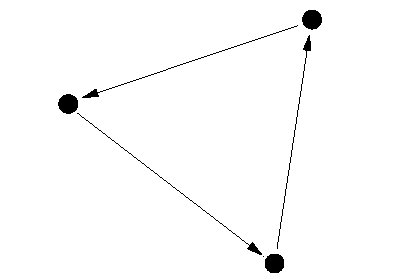
\includegraphics{./sci-pap-roc.pdf}%
\end{picture}%
\setlength{\unitlength}{3947sp}%
%
\begingroup\makeatletter\ifx\SetFigFont\undefined%
\gdef\SetFigFont#1#2#3#4#5{%
  \reset@font\fontsize{#1}{#2pt}%
  \fontfamily{#3}\fontseries{#4}\fontshape{#5}%
  \selectfont}%
\fi\endgroup%
\begin{picture}(3345,2223)(3054,-2286)
\put(5469,-1199){\makebox(0,0)[lb]{\smash{{\SetFigFont{12}{14.4}{\familydefault}{\mddefault}{\updefault}{\color[rgb]{0,0,0}smashes}%
}}}}
\put(5723,-213){\makebox(0,0)[lb]{\smash{{\SetFigFont{12}{14.4}{\familydefault}{\mddefault}{\updefault}{\color[rgb]{0,0,0}scissors}%
}}}}
\put(5381,-2271){\makebox(0,0)[lb]{\smash{{\SetFigFont{12}{14.4}{\familydefault}{\mddefault}{\updefault}{\color[rgb]{0,0,0}rock}%
}}}}
\put(3956,-1652){\makebox(0,0)[lb]{\smash{{\SetFigFont{12}{14.4}{\familydefault}{\mddefault}{\updefault}{\color[rgb]{0,0,0}covers}%
}}}}
\put(4423,-463){\makebox(0,0)[lb]{\smash{{\SetFigFont{12}{14.4}{\familydefault}{\mddefault}{\updefault}{\color[rgb]{0,0,0}cuts}%
}}}}
\put(3069,-837){\makebox(0,0)[lb]{\smash{{\SetFigFont{12}{14.4}{\familydefault}{\mddefault}{\updefault}{\color[rgb]{0,0,0}paper}%
}}}}
\end{picture}%

\end{center}
  
\hint{If at first you don't succeed\ldots \newline
try googling ``scissor paper rock lizard spock.''}

\wbvfill

\workbookpagebreak

\end{enumerate}



%\newpage
%\renewcommand{\bibname}{References for chapter 3}
%\bibliographystyle{plain}
%\bibliography{main}

%% Emacs customization
%% 
%% Local Variables: ***
%% TeX-master: "GIAM-hw.tex" ***
%% comment-column:0 ***
%% comment-start: "%% "  ***
%% comment-end:"***" ***
%% End: ***
 

 
\chapter{Sets}

{\em No more turkey, but I'd like some more of the bread it ate. --Hank Ketcham}


\section{Basic notions of set theory}
%\label{sec:basic_set_notions}



\noindent{\large \bf Exercises --- \thesection\ }

\begin{enumerate}
\item What is the power set of $\emptyset$?  Hint: if you got the last exercise
in the chapter you'd know that this power set has $2^0 = 1$ element.

\hint{The power set of a set always includes the empty set as well as the whole set that we
are forming the power set of.  In this case they happen to coincide so ${\mathcal P}(\emptyset) = \{ \emptyset \}$.  Notice that $2^0 =1$.}

\item Try iterating the power set operator.  What is ${\mathcal P}({\mathcal P}(\emptyset))$?  What is ${\mathcal P}({\mathcal P}({\mathcal P}(\emptyset)))$?

\hint{I won't spoil you're fun, but as a check ${\mathcal P}({\mathcal P}(\emptyset))$ should have $2$ elements, and ${\mathcal P}({\mathcal P}({\mathcal P}(\emptyset)))$ should have $4$.}

\item Determine the following cardinalities.
  \begin{enumerate}
    \item $A = \{ 1, 2, \{3, 4, 5\}\} \quad |A| = $\rule{36pt}{1pt}
    \item $B = \{ \{1, 2, 3, 4, 5\} \} \quad |B| = $\rule{36pt}{1pt}  
  \end{enumerate}

\hint{Three and one}

\item What, in Logic, corresponds the notion $\emptyset$ in Set theory?

\hint{A contradiction.}

\item What, in Set theory, corresponds to the notion $t$ (a tautology) in Logic?

\hint{The universe of discourse.}

\item What is the truth set of the proposition $P(x) = $ ``3 divides $x$ and 2 divides $x$''?

\hint{ The set of all multiples of $6$.}

\item Find a logical open sentence such that $\{0, 1, 4, 9, \ldots \}$ is
its truth set.

\hint{Many answers are possible.  Perhaps the easiest is $\exists y \in \Integers, x = y^2$.}

\item How many singleton sets are there in the power set of 
$\{a,b,c,d,e\}$?  ``Doubleton'' sets?

\hint{5, 10}

\item How many 8 element subsets are there in
\[ {\mathcal P}(\{a,b,c,d,e,f,g,h,i,j,k,l,m,n,o,p\})? \]

\hint{ $\binom{16}{8} = 12870$}

\item How many singleton sets are there in the power set of 
$\{1,2,3, \ldots n\}$?

\hint{$n$}

\end{enumerate}



%% Emacs customization
%% 
%% Local Variables: ***
%% TeX-master: "GIAM-hw.tex" ***
%% comment-column:0 ***
%% comment-start: "%% "  ***
%% comment-end:"***" ***
%% End: ***



\newpage

\section{Containment}



\noindent{\large \bf Exercises --- \thesection\ }

\begin{enumerate}
\item Insert either $\in$ or $\subseteq$ in the blanks in the following 
sentences (in order to produce true sentences).


\begin{tabular}{lcl}
\rule{0pt}{16pt}i) $1$ \underline{\rule{36pt}{0pt}} $\{3, 2, 1, \{a, b\}\}$ & \rule{36pt}{0pt} & iii) $\{a, b\}$  \underline{\rule{36pt}{0pt}} $\{3, 2, 1, \{a, b\}\}$ \\
\rule{0pt}{16pt}ii) $\{a\}$ \underline{\rule{36pt}{0pt}} $\{a, \{a, b\}\}$ & &
iv) $\{\{a, b\}\}$  \underline{\rule{36pt}{0pt}} $\{a, \{a, b\}\}$ \\
\end{tabular}

\hint{$\in$, $\subseteq$, $\in$, $\subseteq$}

\item  Suppose that $p$ is a prime, for each $n$ in $\Integers^+$, 
define the set $P_n = \{ x \in \Integers^+ \suchthat \, p^n \divides x \}$.  
Conjecture and prove a statement about the containments between these sets.

\hint{When $p=2$ we have seen these sets.  $P_1$ is the even numbers, $P_2$ is the doubly-even numbers,
etc.}

\wbvfill

\item  Provide a counterexample to dispel the notion that a subset must
have fewer elements than its superset.

\hint{A subset is called {\em proper} if it is neither empty nor equal to the superset.   If
we are talking about finite sets then the proper subsets do indeed have fewer elements
than the supersets.  Among infinite sets it is possible to have proper subsets having the same 
number of elements as their superset, for example there are just as many even natural numbers
as there are natural numbers all told.}

\wbvfill

\workbookpagebreak

\item  We have seen that $A \subseteq B$ corresponds to $M_A \implies M_B$.
What corresponds to the contrapositive statement?

\hint{Turn ``logical negation'' into ``set complement'' and reverse the direction of the inclusion.}
 
\wbvfill

\item Determine two sets $A$ and $B$ such that both of the sentences
$A \in B$ and $A \subseteq B$ are true.

\hint{The smallest example I can think of would be $A=\emptyset$ and $B=\{\emptyset\}$.  You should come up with a different example.}

\wbvfill

\item Prove that the set of perfect fourth powers is contained in the
set of perfect squares.

\hint{It would probably be helpful to have precise definitions of the sets described in the problem.

The fourth powers are
\[ F = \{x \suchthat \exists y \in \Integers, x=y^4 \}. \]

The squares are 
\[ S = \{x \suchthat \exists z \in \Integers, x=z^2 \}. \]

To show that one set is contained in another, we need to show that the first set's membership
criterion implies that of the second set.}

\wbvfill

\end{enumerate}



%% Emacs customization
%% 
%% Local Variables: ***
%% TeX-master: "GIAM-hw.tex" ***
%% comment-column:0 ***
%% comment-start: "%% "  ***
%% comment-end:"***" ***
%% End: ***



\newpage

\begin{table}[hbt] 
\begin{center}
\begin{tabular}{c|c|c} 
 & \begin{minipage}{.35\textwidth} \centerline{Intersection}
\centerline{\rule[-10pt]{0pt}{10pt}version} \end{minipage} & 
\begin{minipage}{.35\textwidth} \centerline{Union}
\centerline{\rule[-10pt]{0pt}{10pt}version} \end{minipage} \\ \hline
\begin{minipage}{.25\textwidth} \rule{0pt}{22pt}Commutative \\ \rule{12pt}{0pt} laws\rule[-10pt]{0pt}{10pt} \end{minipage} & 
\begin{minipage}{.35\textwidth} \centerline{$A \cap B = B \cap A$} \end{minipage} & 
\begin{minipage}{.35\textwidth} \centerline{$A \cup B = B \cup A$} \end{minipage} \\ \hline
\begin{minipage}{.25\textwidth} \rule{0pt}{22pt}Associative \\ \rule{12pt}{0pt} laws\rule[-10pt]{0pt}{10pt} \end{minipage} & 
\begin{minipage}{.35\textwidth} \centerline{$A \cap (B \cap C)$\rule{26pt}{0pt}} 
\centerline{\rule{26pt}{0pt} $= (A \cap B) \cap C $}\end{minipage} &
\begin{minipage}{.35\textwidth} \centerline{$A \cup (B \cup C)$ \rule{26pt}{0pt}}
\centerline{\rule{26pt}{0pt} $= (A \cup B) \cup C $} \end{minipage} \\ \hline 
\begin{minipage}{.25\textwidth} \rule{0pt}{22pt}Distributive \\ \rule{12pt}{0pt} laws\rule[-10pt]{0pt}{10pt} \end{minipage} &  
\begin{minipage}{.35\textwidth} 
\centerline{$A \cap (B \cup C) = $ \rule{26pt}{0pt}} 
\centerline{\rule{16pt}{0pt}$(A \cap B) \cup (A \cap C)$} \end{minipage} & 
\begin{minipage}{.35\textwidth} \centerline{$A \cup (B \cap C) = $ \rule{26pt}{0pt}} 
\centerline{\rule{16pt}{0pt}$(A \cup B) \cap (A \cup C)$} \end{minipage} \\ \hline 
\begin{minipage}{.25\textwidth} \rule{0pt}{22pt}DeMorgan's \\ \rule{12pt}{0pt} laws\rule[-10pt]{0pt}{10pt} \end{minipage} & 
\begin{minipage}{.35\textwidth} \centerline{$\overline{A \cap B}$ \rule{25pt}{0pt}}
\centerline{ \rule{16pt}{0pt} $ = \; \overline{A} \cup \overline{B}$} \end{minipage} & 
\begin{minipage}{.35\textwidth} \centerline{$\overline{A \cup B}$\rule{25pt}{0pt}}
\centerline{ \rule{16pt}{0pt} $= \; \overline{A} \cap \overline{B}$} \end{minipage} \\ \hline 
\begin{minipage}{.25\textwidth} \rule{0pt}{22pt}Complementarity\rule[-10pt]{0pt}{10pt} \end{minipage} & 
\begin{minipage}{.35\textwidth} \centerline{$A \cap \overline{A} \; = \; \emptyset$} \end{minipage} & 
\begin{minipage}{.35\textwidth} \centerline{$A \cup \overline{A} \; = \; U$} \end{minipage} \\ \hline 
\begin{minipage}{.25\textwidth} \rule{0pt}{22pt}Identity \\ \rule{12pt}{0pt} laws\rule[-10pt]{0pt}{10pt} \end{minipage} & 
\begin{minipage}{.35\textwidth} \centerline{$A \cap U = A$} \end{minipage} & 
\begin{minipage}{.35\textwidth} \centerline{$A \cup \emptyset = A$} \end{minipage} \\ \hline 
\begin{minipage}{.25\textwidth} \rule{0pt}{22pt}Domination\rule[-10pt]{0pt}{10pt} \end{minipage} & 
\begin{minipage}{.35\textwidth}  \centerline{$A \cap \emptyset = \emptyset$} \end{minipage} & 
\begin{minipage}{.35\textwidth} \centerline{$A \cup U = U$} \end{minipage} \\ \hline
\begin{minipage}{.25\textwidth} \rule{0pt}{22pt}Idempotence\rule[-10pt]{0pt}{10pt} \end{minipage} & 
\begin{minipage}{.35\textwidth} \centerline{$A \cap A = A$} \end{minipage} & 
\begin{minipage}{.35\textwidth} \centerline{$A \cup A = A$} \end{minipage} \\ \hline
\begin{minipage}{.25\textwidth} \rule{0pt}{22pt}Absorption\rule[-10pt]{0pt}{10pt} \end{minipage} & 
\begin{minipage}{.35\textwidth} \centerline{$A \cap (A \cup B) = A$} \end{minipage} & 
\begin{minipage}{.35\textwidth} \centerline{$A \cup (A \cap B) = A$} \end{minipage} \\
\end{tabular} 
\end{center} 
\caption{Basic set theoretic equalities.}
\index{set theoretic equalities}
\label{tab:set_equiv}
\end{table}

%% Emacs customization
%% 
%% Local Variables: ***
%% TeX-master: "GIAM-hw.tex" ***
%% comment-column:0 ***
%% comment-start: "%% "  ***
%% comment-end:"***" ***
%% End: ***



\clearpage

\section{Set operations}

\noindent{\large \bf Exercises --- \thesection\ }

\begin{enumerate}
\item Let $A = \{1, 2, \{1, 2\}, b\}$ and let $B=\{a, b, \{1, 2\} \}$.
Find the following:
  \begin{enumerate}
  \item $A \cap B$   \hint{ $ \{ b,  \{1, 2\} \} $ }
  \item $A \cup B$ \hint{ $ \{1, 2, a, b, \{1, 2\} \} $ }
  \item $A \setminus B$ \hint{  $ \{ 1, 2 \} $ }
  \item $B \setminus A$ \hint{ $ \{ a \} $ }
  \item $A \triangle B$ \hint{ $ \{ 1, 2, a \} $ }
  \end{enumerate}

\vfill

\item In a standard deck of playing cards one can distinguish sets
based on face-value and/or suit.  Let $A, 2, \ldots 9, 10, J, Q$ and $K$
represent the sets of cards having the various face-values.  Also, let
$\heartsuit$, $\spadesuit$, $\clubsuit$ and $\diamondsuit$ be the 
sets of cards having the possible suits.  Find the following
  \begin{enumerate}
  \item $A \cap \heartsuit$ \hint{This is just the ace of hearts.}
  \item $A \cup \heartsuit$ \hint{All of the hearts and the other three aces}
  \item $J \cap (\spadesuit \cup \heartsuit)$ \hint{ These two cards are known as the one-eyed jacks.}
  \item $K \cap \heartsuit$ \hint{The king of hearts, a.k.a. the suicide king.}
  \item $A \cap K$ \hint{$\emptyset$ }
  \item $A \cup K$ \hint{Eight cards: all four kings and all four aces.}
  \end{enumerate}

\vfill

\hintspagebreak

\item Do element-chasing proofs (show that an element is in the left-hand side if and only if it is in the right-hand side) to prove each of the following set equalities.  

  \begin{enumerate}
  \item $\overline{A\cap B} \; = \; \overline{A}\cup\overline{B}$

  \item $A\cup B \; = \; A\cup(\overline{A}\cap B)$

  \item $A\triangle B \; = \; (A\cup B)\setminus(A\cap B)$

  \item $(A\cup B)\setminus C \; = \; (A\setminus C)\cup(B\setminus C)$

  \end{enumerate}

\hint{Here's the first one (although I'm omiting justifications for each step.

\begin{gather*}
x \in \overline{A\cap B} \\
\iff \; {\lnot}(x \in A\cap B) \\
\iff \; {\lnot}(x \in A \; \land \; x \in B) \\
\iff \; {\lnot}(x \in A) \; \lor \; {\lnot}(x \in B) \\
\iff \; x \in \overline{A}  \; \lor \; x \in \overline{B} \\
\iff \; x \in \overline{A} \cup \overline{B}
\end{gather*}
}



\item For each positive integer $n$, we'll define an interval $I_n$
by

\[ I_n = [-n, 1/n). \]

Find the union and intersection of all the intervals in this infinite family.

\[ \bigcup_{n \in \Naturals} I_n \quad = \]

\[ \bigcap_{n \in \Naturals} I_n \quad = \]

\hint{To better understand what is going on, first figure out what the first three or four
intervals actually are.

\[ I_1 \; = \; \underline{\rule{96pt}{0pt}} \]
\[ I_2 \; = \; \underline{\rule{96pt}{0pt}} \]
\[ I_3 \; = \; \underline{\rule{96pt}{0pt}} \]
\[ I_4 \; = \; \underline{\rule{96pt}{0pt}} \]

Any negative real number $r$ will be in the intersection only if  $r \geq -1$.  Certainly $0$ is in
the intersection since it is in each of the intervals.  Are there any positive numbers in the intersection?

In order to be in the union a real number just needs to be in {\em one} of the intervals.
}

\item There is a set $X$ such that, for all sets $A$, we have 
$X \triangle A = A$.  What is $X$?

\item There is a set $Y$ such that, for all sets $A$, we have 
$Y \triangle A = \overline{A}$.  What is $Y$?

\hint{One of the answers to the last two questions is $\emptyset$ and the other is $U$.  Decide
which is which.}

\item In proving a set-theoretic identity, we are basically showing that
two sets are equal.  One reasonable way to proceed is to show that
each is contained in the other.  Prove that 
$A \cap (B \cup C) = (A \cap B) \cup (A \cap C)$ by showing that 
$A \cap (B \cup C) \subseteq (A \cap B) \cup (A \cap C)$ and 
$(A \cap B) \cup (A \cap C) \subseteq A \cap (B \cup C)$.

\item Prove that 
$A \cup (B \cap C) = (A \cup B) \cap (A \cup C)$ by showing that 
$A \cup (B \cap C) \subseteq (A \cup B) \cap (A \cup C)$ and 
$(A \cup B) \cap (A \cup C) \subseteq A \cup (B \cap C)$.

\hint{This exercise, as well as the previous one, is really just about converting set-theoretic
statements into their logical equivalents, applying some rules of logic that we've already verified,
and then returning to a set-theoretic version of things.}
 
\item Prove the set-theoretic versions of DeMorgan's laws using the technique
discussed in the previous problems.

\item The previous technique (showing that $A=B$ by arguing that
$A \subseteq B \; \land \; B \subseteq A$) will have an outline something like

\begin{proof} 
First we will show that $A \subseteq B$.\newline
Towards that end, suppose $x \in A$.

\begin{center}
$\vdots$
\end{center}

Thus $x \in B$.

Now, we will show that $B \subseteq A$. \newline
Suppose that $x \in B$.

\begin{center}
$\vdots$
\end{center}

Thus $x \in A$.

Therefore $A \subseteq B \; \land \; B \subseteq A$ so we conclude that $A=B$.
\end{proof}

Formulate a proof that $A \triangle B \; = \; (A \cup B) \setminus (A \cap B)$.

\hint{The definition of $A \triangle B$ is $(A\setminus B) \cup (B\setminus A)$.  The definition of 
$X \setminus Y$ is $X \cap \overline{Y}$.   Restating things in terms of $\cap$ and $\cup$ (and complementation) should help.  So your first few lines should be:

 \begin{quote} 
 Suppose $x \in  A \triangle B$.  
 
Then, by definition, $x \in (A\setminus B) \cup (B\setminus A)$.
 
 So, $x \in (A \cap \overline{B}) \cup (B \cap \overline{A})$.
   
\begin{center}
$\vdots$
\end{center}

\end{quote}
}

\end{enumerate}


%% Emacs customization
%% 
%% Local Variables: ***
%% TeX-master: "GIAM-hw.tex" ***
%% comment-column:0 ***
%% comment-start: "%% "  ***
%% comment-end:"***" ***
%% End: ***




\clearpage

\section{Venn diagrams}

\noindent{\large \bf Exercises --- \thesection\ }

\begin{enumerate}
\item  Venn diagrams are usually made using simple closed curves 
with no further restrictions.  Try creating Venn diagrams for 3, 4 and
5 sets (in general position) using rectangular simple closed curves.

\hint{I found it easier to experiment by making my drawings on graph paper.  I never did  
manage to draw the $5$ set Venn diagram with just rectangles\ldots probably just a lack of persistence.}

\item  We call a curve \emph{rectilinear} if it is made
of line segments that meet at right angles.  Use rectilinear
simple closed curves to create a Venn diagram for 5 sets.

\hint{Of course, rectangles are rectilinear, so one could use the solution from the previous
problem (if, unlike me, you were persistant enough to find it).  Otherwise, 
start with the $4$ set diagram made with rectangles and use your $5$th (rectilinear) curve to split
each region into $2$ -- don't forget to split the region on the outside too.}

\item  Argue as to why rectilinear curves will suffice to build
any Venn diagram.

\hint{Fortunately the instructions don't say to {\em prove} that rectilinear curves will always
suffice, so we can be less rigorous.  Try to argue as to why it will alway be possible to add one more rectilinear curve to an existing Venn diagram and split every region into two.}

\item  Find the disjunctive normal form of $A \cap (B \cup C)$.

\hint{ $ (A \cap B \cap \overline{C}) \cup (A \cap \overline{B} \cap C) $ }

\item  Find the disjunctive normal form of $(A \triangle B) \triangle C$

\hint{It is $(A \cap \overline{B} \cap \overline{C}) \cup (\overline{A} \cap B \cap \overline{C}) \cup (\overline{A} \cap \overline{B} \cap C)$.  Now find the disjunctive normal form of 
$A \triangle (B \triangle C)$.}

\item The prototypes for the \emph{modus ponens} and \emph{modus tollens}
argument forms are the following:

\begin{tabular}{lcl}
\begin{minipage}{.3\textwidth}All men are mortal. \newline %
Socrates is a man. \newline
Therefore Socrates is mortal.\end{minipage} & \rule{16pt}{0pt} and \rule{16pt}{0pt} & %
 \begin{minipage}{.3\textwidth}All men are mortal. \newline %
Zeus is not mortal. \newline
Therefore Zeus is not a man.\end{minipage}
\end{tabular}

Illustrate these arguments using Venn diagrams.

\hint{The statement ``All men are mortal'' would be interpreted on a Venn diagram by showing the
set of ``All men'' as being entirely contained within the set of ``mortal beings.''   Socrates is an 
element of the inner set.  Zeus, on the other hand, lies outside of the outer set.}
 
\item Use Venn diagrams to convince yourself of the validity of
the following containment statement

\[ (A \cap B) \cup (C \cap D) \; \subseteq \; (A \cup C) \cap (B \cup D).\]

Now prove it!
 
\hint{Obviously we'll need one of the $4$-set Venn diagrams.}
 
\item Use Venn diagrams to show that the following set equivalence is false.

\[ (A \cup B) \cap (C \cup D) \; = \; (A \cup C) \cap (B \cup D) \]

\hint{After constructing Venn diagrams for both sets you should be able to see that there
are $4$ regions where they differ.  One is $A \cap B \cap \overline{C} \cap \overline{D}$.
What are the other three?}

\end{enumerate}



%% Emacs customization
%% 
%% Local Variables: ***
%% TeX-master: "GIAM-hw.tex" ***
%% comment-column:0 ***
%% comment-start: "%% "  ***
%% comment-end:"***" ***
%% End: ***



\newpage

\section{Russell's Paradox}
%\label{sec:russell}

\noindent{\large \bf Exercises --- \thesection\ }

\begin{enumerate}
\item Verify that $(A \implies {\lnot}A) \land ({\lnot}A \implies A)$
is a logical contradiction in two ways:  by filling out a truth table and 
using the laws of logical equivalence.

\hint{In order to get started on this you'll need to convert the conditionals into equivalent
disjunctions.  Recall that $X \implies Y \; \equiv \; {\lnot}X \lor Y$.}

\item One way out of Russell's paradox is to declare that the collection
of sets that don't contain themselves as elements is not a set itself.
Explain how this circumvents the paradox. 

\hint{If it's not a set then it doesn't necessarily have to have the property that we
can be {\em sure} whether an element is in it or not.}

\end{enumerate}


%% Emacs customization
%% 
%% Local Variables: ***
%% TeX-master: "GIAM-hw.tex" ***
%% comment-column:0 ***
%% comment-start: "%% "  ***
%% comment-end:"***" ***
%% End: ***




%% Emacs customization
%% 
%% Local Variables: ***
%% TeX-master: "GIAM-hw.tex" ***
%% comment-column:0 ***
%% comment-start: "%% "  ***
%% comment-end:"***" ***
%% End: ***



\chapter{Proof techniques II --- Induction}


\section{The principle of mathematical induction}
\label{sec:induct}


\noindent{\large \bf Exercises --- \thesection\ }

\begin{enumerate}
\item Consider the sequence of number that are 1 greater than a multiple of 4.
(Such numbers are of the form $4j+1$.)

\[ 1, 5, 9, 13, 17, 21, 25, 29, \ldots \]

The sum of the first several numbers in this sequence can be expressed as
a polynomial.

\[ \sum_{j=0}^n 4j+1 = 2n^2 + 3n + 1 \]

Complete the following table in order to provide evidence that the formula
above is correct.

\begin{center}
\begin{tabular}{c|c|c}
$n$ & $\sum_{j=0}^n 4j+1$ & $2n^2 + 3n + 1$ \\ \hline
 0 & $1$ & $1$ \\
 1 & $1 + 5 = 6$ &  $2 \cdot 1^2 + 3 \cdot 1 + 1 = 6$ \\
 2 & $1 + 5 + 9 = \rule{15pt}{0pt}$ \hint{$15$} &  \hint{$2 \cdot 2^2 + 3 \cdot 2 + 1 = 15$}\\
 3 & \hint{$1 + 5 + 9 + 13 = 28$} &  \hint{$2 \cdot 3^2 + 3 \cdot 3 + 1 = 28$}\\
 4 & & \\
\end{tabular}
\end{center}

\hint{I'm leaving the very last one for you to do.}


\item \label{ex:horses} What is wrong with the following inductive proof of
``all horses are the same color.''?

{\bf Theorem} Let $H$ be a set of $n$ horses, all horses in $H$ 
are the same color.

\begin{proof}
We proceed by induction on $n$.

\noindent {\bf Basis: } Suppose $H$ is a set containing 1 horse.  Clearly
this horse is the same color as itself.

\noindent {\bf Inductive step: } Given a set of $k+1$ horses $H$ we can 
construct two sets of $k$ horses.  Suppose $H = \{ h_1, h_2, h_3, \ldots h_{k+1} \}$.  Define $H_a = \{ h_1, h_2, h_3, \ldots h_{k} \}$ (i.e. $H_a$ contains
just the first $k$ horses) and $H_b = \{ h_2, h_3, h_4, \ldots h_{k+1} \}$ 
(i.e. $H_b$ contains the last $k$ horses).  By the inductive hypothesis
both these sets contain horses that are ``all the same color.''  Also,
all the horses from $h_2$ to $h_k$ are in both sets so both $H_a$ and
$H_b$ contain only horses of this (same) color.  Finally, we conclude that
all the horses in $H$ are the same color.

\end{proof}
\medskip
   
\hint{Look carefully at the stage from $n=2$ to $n=3$.}

\hintspagebreak

\item For each of the following theorems, write the statement that must be
proved for the basis -- then prove it, if you can!

\begin{enumerate}
\item The sum of the first $n$ positive integers is $(n^2+n)/2$.

\hint{The sum of the first $0$ positive integers is $(0^2 + 0)/2$.  Or, if you
prefer to start with something rather than nothing: The sum of the first $1$ positive integers
is $(1^2+1)/2$. }

\item The sum of the first $n$ (positive) odd numbers is $n^2$.

\hint{The sum of the first $0$ positive odd numbers is $0^2$.  Or, the sum of the first $1$ positive odd numbers is $1^2$.}

\item If $n$ coins are flipped, the probability that all of them 
are ``heads'' is $1/2^n$.

\hint{If $1$ coin is flipped, the the probability that it is ``heads'' is $1/2$. Or if we try it 
when $n=0$, ``If no coins are flipped the probability that all t=of them are heads is 1.  Does that
make sense to you?  Is it reasonable that we would say it is 100\% certain that all of the coins
are heads in a set that doesn't contain {\em any} coins? }

\item Every $2^n \times 2^n$ chessboard -- with one square removed -- can 
be tiled perfectly\footnote{Here, ``perfectly tiled'' means that every trominoe
covers 3 squares of the chessboard (nothing hangs over the edge) and that every
square of the chessboard is covered by some trominoe.} by L-shaped trominoes.  
(A trominoe is like a domino but 
made up of $3$ little squares.  There are two kinds, straight 
\begin{picture}(0,0)%
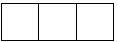
\includegraphics{figures/straight_trominoe.pdf}%
\end{picture}%
\setlength{\unitlength}{3947sp}%
%
\begingroup\makeatletter\ifx\SetFigFont\undefined%
\gdef\SetFigFont#1#2#3#4#5{%
  \reset@font\fontsize{#1}{#2pt}%
  \fontfamily{#3}\fontseries{#4}\fontshape{#5}%
  \selectfont}%
\fi\endgroup%
\begin{picture}(924,324)(1189,-673)
\end{picture}%
 and L-shaped 
\begin{picture}(0,0)%
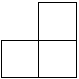
\includegraphics{figures/L-shaped_trominoe.pdf}%
\end{picture}%
\setlength{\unitlength}{3947sp}%
%
\begingroup\makeatletter\ifx\SetFigFont\undefined%
\gdef\SetFigFont#1#2#3#4#5{%
  \reset@font\fontsize{#1}{#2pt}%
  \fontfamily{#3}\fontseries{#4}\fontshape{#5}%
  \selectfont}%
\fi\endgroup%
\begin{picture}(624,624)(1189,-673)
\end{picture}%
. This problem is only concerned with
the L-shaped trominoes.)
\end{enumerate}

\hint{If $n=1$ we have: ``Every $2 \times 2$ chessboard -- with one square removed
can be tiled perfectly by L-shaped trominoes.  This version is trivial to prove.  Try formulating
the $n=0$ case.}
  
\hintspagebreak

\item Suppose that the rules of the game for PMI were changed so that one
did the following:
\begin{itemize}
\item Basis.  Prove that $P(0)$ is true.
\item Inductive step.  Prove that for all $k$, $P_k$ implies $P_{k+2}$
\end{itemize}


\noindent Explain why this would not constitute a valid proof that $P_n$ holds 
for all natural numbers $n$. 
\noindent How could we change the basis in this outline to obtain a valid proof?

\hint{In this modified version, $P(0)$ is not going to imply $P(1)$. and in fact, none of the odd numbered
statements will be proven.  If we change the 
basis so that we prove both $P(0$ and $P(1)$, all the even statements will be implied by
$P(0$ being true and all the odd statements get forced because $P(1)$ is true.}

\item If we wanted to prove statements that were indexed by the integers,

\[ \forall z \in \Integers, \; P_z, \]

\noindent what changes should be made to PMI?

\hint{A quick change would be to replace $\forall k, \; P_k \implies P_{k+1}$ in the inductive
step with $\forall k, \; P_k \iff P_{k+1}$.  While this would do the trick, a slight improvement 
is possible, if we treat the positive and negative cases for $k$ seperately.}
 
\end{enumerate}


%% Emacs customization
%% 
%% Local Variables: ***
%% TeX-master: "GIAM-hw.tex" ***
%% comment-column:0 ***
%% comment-start: "%% "  ***
%% comment-end:"***" ***
%% End: ***




 
\newpage

\section{Formulas for sums and products}


\noindent{\large \bf Exercises --- \thesection\ }

\begin{enumerate}
\item Write an inductive proof of the formula for the sum 
of the first $n$ cubes.

\hint{
\begin{thm*}
\[ \forall n \in \Naturals, \; \sum_{k=1}^n k^3 \;= \; \left( \frac{n(n+1)}{2} \right)^2 \]
\end{thm*}

\begin{proof} (By mathematical induction)

{\bf Base case:} ($n=1$)
For the base case, note that when $n=1$ we have

\[ \sum_{k=1}^n k^3 \; = \; 1 \]

\noindent and 

\[ \left( \frac{n(n+1)}{2} \right)^2  \; = \; 1.\]

{\bf Inductive step:}

Suppose that $m>1$ is an integer such that 

\[ \sum_{k=1}^m k^3 \; = \; \left( \frac{m(m+1)}{2} \right)^2 \]

\noindent Add $(m+1)^3$ to both sides to obtain

\[ (m+1)^3 + \sum_{k=1}^m k^3 \;= \; \left( \frac{m(m+1)}{2} \right)^2 + (m+1)^3. \]

\noindent Thus

\begin{gather*} 
\sum_{k=1}^{m+1} k^3 \;= \; \left( \frac{m^2(m+1)^2}{4} \right) + \frac{4(m+1)^3}{4} \\
\;= \; \left( \frac{m^2(m+1)^2 + 4 (m+1)^3}{4} \right)\\
\; = \; \left( \frac{(m+1)^2 (m^2 + 4(m+1))}{4} \right)\\
\; = \; \left( \frac{(m+1)^2 (m^2 + 4m +4)}{4} \right)\\
\; = \; \left( \frac{(m+1)^2 (m+2)^2}{4} \right)\\
\; = \; \left( \frac{(m+1)(m+2)}{2} \right)^2
\end{gather*}

 \end{proof}
}

\wbvfill

\workbookpagebreak
  
\item Find a formula for the sum of the first $n$ fourth powers.

\hint{\[ \frac{n\cdot(n+1)\cdot(2n+1)\cdot(3n^2+3n-1)}{30}\] } 

\wbvfill

\workbookpagebreak
 
\item The sum of the first $n$ natural numbers is sometimes called
the $n$-th triangular number \index{triangular numbers}$T_n$.  Triangular numbers are so-named
because one can represent them with triangular shaped arrangements 
of dots. 

\begin{center} \begin{picture}(0,0)%
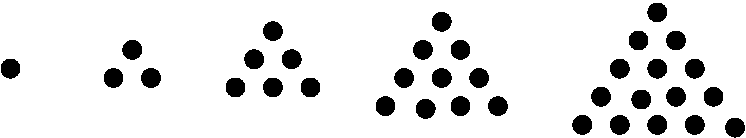
\includegraphics{./triangular_numbers.pdf}%
\end{picture}%
\setlength{\unitlength}{3947sp}%
%
\begingroup\makeatletter\ifx\SetFigFont\undefined%
\gdef\SetFigFont#1#2#3#4#5{%
  \reset@font\fontsize{#1}{#2pt}%
  \fontfamily{#3}\fontseries{#4}\fontshape{#5}%
  \selectfont}%
\fi\endgroup%
\begin{picture}(5963,1088)(1193,-2116)
\end{picture}%
 \end{center}

The first several triangular numbers are 1, 3, 6, 10, 15, et cetera.

Determine a formula for the sum of the first $n$ triangular numbers $\displaystyle \left( \sum_{i=1}^n T_i \right)$ and prove it using PMI.

\hint{The formula is $\frac{n(n+1)(n+2)}{6}$.}

\wbvfill

\workbookpagebreak

\item Consider the alternating sum of squares:
\begin{gather*}
1 \\
1 - 4 = -3 \\
1 - 4 + 9 = 6 \\
1 - 4 + 9 - 16 = -10 \\
\mbox{et cetera}
\end{gather*}
Guess a general formula for $\sum_{i=1}^n (-1)^{i-1} i^2$, and prove it using PMI.

\hint{
\begin{thm*}
\[ \forall n \in \Naturals, \; \sum_{i=1}^n (-1)^{i-1} i^2 \;= \; (-1)^{n-1} \frac{n(n+1)}{2}  \]
\end{thm*}

\begin{proof} (By mathematical induction)

{\bf Base case:} ($n=1$)
For the base case, note that when $n=1$ we have

\[\sum_{i=1}^n (-1)^{i-1} i^2 \;= \; 1 \]

\noindent and also

\[ (-1)^{n-1} \frac{n(n+1)}{2} \;= \; 1. \]

{\bf Inductive step:}

Suppose that $k>1$ is an integer such that 

\[ \sum_{i=1}^k (-1)^{i-1} i^2 \;= \; (-1)^{k-1} \frac{k(k+1)}{2}.  \]

Adding $(-1)^{k} (k+1)^2$ to both sides gives

\begin{gather*} 
\sum_{i=1}^{k+1} (-1)^{i-1} i^2 \;= \; (-1)^{k-1} \frac{k(k+1)}{2} + (-1)^{k} (k+1)^2 \\
\;= \; (-1)^{k-1} \frac{k(k+1)}{2} - (-1)^{k-1} (k+1)^2 \\ 
\;= \; (-1)^{k-1} \left( \frac{k(k+1)}{2} -  \frac{2(k+1)^2}{2} \right) \\ 
\;= \; (-1)^{k} \left( \frac{2(k+1)^2}{2} - \frac{k(k+1)}{2} \right) \\
\;= \; (-1)^{k} \frac{(k+1)(2(k+1)-k)}{2} \\
\;= \; (-1)^{k} \frac{(k+1)(k+2)}{2} \\
\end{gather*}
\end{proof}
}

\wbvfill

\workbookpagebreak

\item Prove the following formula for a product.

\[ \prod_{i=2}^n \left(1 - \frac{1}{i}\right) =  \frac{1}{n} \]

\hint{
Notice that the problem statement didn't specify the domain -- but the smallest value of $n$ that gives
a non-empty product on the left-hand side is $n=2$.  

\newpage

\begin{proof} (By mathematical induction)

{\bf Base case:} ($n=2$)
For the base case, note that when $n=2$ we have

\[ \prod_{i=2}^2 \left(1 - \frac{1}{i}\right) \quad = \quad  \left(1 - \frac{1}{2}\right) \quad = \quad 1/2 \]

\noindent and, when $n=2$, the right-hand side ($1/n$) also evaluates to $1/2$.

{\bf Inductive step:}

Suppose that $k\geq2$ is an integer such that 

\[ \prod_{i=2}^k \left(1 - \frac{1}{i}\right) =  \frac{1}{k}. \]

Then,

\begin{gather*}
\prod_{i=2}^{k+1} \left(1 - \frac{1}{i}\right) \\
= \left(1 - \frac{1}{k+1}\right) \; \cdot \; \prod_{i=2}^{k} \left(1 - \frac{1}{i}\right) \\
= \left(1 - \frac{1}{k+1}\right) \; \cdot \; \frac{1}{k} \\
= \frac{1}{k+1}.
\end{gather*}
\end{proof}

The final line skips over a tiny bit of algebraic detail.  You may feel more comfortable if you fill in those steps.

\newpage
}


\item Prove $\displaystyle \sum_{j=0}^{n}(4j+1) \; = \; 2n^{2}+3n+1$ for all
integers $n \geq 0$.

\hint{
\begin{proof} (By mathematical induction)

{\bf Base case:} ($n=0$)
For the base case, note that when $n=0$ we have

\[ \sum_{j=0}^{n}(4j+1) \; = \; (4\cdot 0 + 1 \; = \; 1 \]

\noindent also, when $n=0$,

\[ 2n^2+3n+1 \; = \; 2\cdot 0^2 +3\cdot 0 + 1 \; = \; 1. \]

{\bf Inductive step:}

Suppose that $k \geq 0$ is an integer such that 

\[  \sum_{j=0}^{k}(4j+1) \; = \; 2k^{2}+3k+1. \]

(We want to show that $\displaystyle \sum_{j=0}^{k+1}(4j+1) \; = \; 2(k+1)^{2}+3(k+1)+1$.)

So consider the sum $\displaystyle \sum_{j=0}^{k+1}(4j+1)$:

\begin{gather*}
\sum_{j=0}^{k+1}(4j+1) \\
= \; 4(k+1)+1 \; + \; \sum_{j=0}^{k}(4j+1) \\
= \;  4(k+1)+1 \; + \; 2k^{2}+3k+1 \\
= \; \rule{0pt}{18pt} \rule{2in}{0pt} \\
= \; \rule{0pt}{18pt} \rule{2in}{0pt} \\
= \; \rule{0pt}{18pt} \rule{2 in}{0pt} \\
\end{gather*}
\end{proof}


Notice that the last line given in the proof is where the inductive hypothesis gets used.  The actual last line of the proof is fairly easy to determine (hint: it is given in the "We want to show" sentence.)  So now you just have to fill in the gaps\ldots

\rule{0pt}{12pt}

}

\wbvfill

\workbookpagebreak

\item Prove $\displaystyle \sum_{i=1}^{n}\frac{1}{(2i-1)(2i+1)} \; = \; \frac{n}{2n+1}$ for all natural numbers $n$.

\hint{
\begin{proof} (By mathematical induction)

{\bf Base case:} ($n=0$)
For the base case, note that when $n=0$ 

\[ \sum_{j=0}^{n} \frac{1}{(2i-1)(2i+1)} \]

contains no terms. Thus its value is 0.

And, $\displaystyle \frac{n}{2n+1}$ also evaluates to 0 when $n=0$.

{\bf Inductive step:}

By the inductive hypothesis we may write

\[ \sum_{i=1}^{k} \frac{1}{(2i-1)(2i+1)} \; = \; \frac{k}{2k+1}. \]

Adding $\displaystyle  \frac{1}{(2(k+1)-1)(2(k+1)+1)}$ to both side of this gives

\[ \sum_{i=1}^{k+1} \frac{1}{(2i-1)(2i+1)} \; = \; \frac{k}{2k+1} \; + \; \frac{1}{(2(k+1)-1)(2(k+1)+1)}. \]

To complete the proof we must verify that 

\[ \frac{k}{2k+1} \; + \; \frac{1}{(2(k+1)-1)(2(k+1)+1)} = \frac{k+1}{2(k+1)+1}. \]

Note that
\begin{gather*}
\rule{0pt}{23pt} \frac{k}{2k+1} \; + \; \frac{1}{(2(k+1)-1)(2(k+1)+1)} \\
\rule{0pt}{23pt} = \frac{k}{2k+1} \; + \; \frac{1}{(2k+1)(2k+3)}\\
\rule{0pt}{23pt} = \frac{k(2k+3)}{(2k+1)(2k+3)} \; + \; \frac{1}{(2k+1)(2k+3)}\\
\rule{0pt}{23pt} = \frac{k(2k+3)+1}{(2k+1)(2k+3)} \\
\rule{0pt}{23pt} = \frac{2k^2+3k+1}{(2k+1)(2k+3)} \\
\rule{0pt}{23pt} = \frac{(2k+1)(k+1)}{(2k+1)(2k+3)} \\
\rule{0pt}{23pt} = \frac{k+1}{2k+3} \; = \; \frac{k+1}{2(k+1)+1}
\end{gather*}

\noindent as desired.


\end{proof}

}
\wbvfill

\workbookpagebreak

\item The \index{Fibonacci numbers} \emph{Fibonacci numbers} are a sequence of integers defined by
the rule that a number in the sequence is the sum of the two that 
precede it.

\[ F_{n+2} = F_n + F_{n+1}  \]

\noindent The first two Fibonacci numbers (actually the zeroth and the first) 
are both 1.  

\noindent Thus, the first several Fibonacci numbers are

\[ F_0 = 1, F_1=1, F_2=2, F_3=3, F_4=5, F_5=8, F_6=13, F_7=21, \; \mbox{et cetera} \]

Use mathematical induction to prove the following formula involving
Fibonacci numbers.

\[ \sum_{i=0}^n (F_i)^2 \, = \, F_n \cdot F_{n+1} \]

\hint{
\begin{proof} (by induction)

{\bf Base case:} ($n=0$)

For the base case, note that when $n=0$ 

\[ \sum_{i=0}^{n} (F_i)^2 \; = \; 1. \]

And, $\displaystyle F_n \cdot F_{n+1} \; = \; F_0 \cdot F_1 \; = \; 1 \cdot 1 \; = \; 1$. 

{\bf Inductive step:}

By the inductive hypothesis we may write

\[ \sum_{i=0}^k (F_i)^2 \; = \; F_k \cdot F_{k+1}. \]

Adding $(F_{k+1})^2$ to both sides gives

\[ \sum_{i=0}^{k+1} (F_i)^2 \; = \; F_k \cdot F_{k+1} + (F_{k+1})^2. \]

Finally, note that (using factoring and the defining property of the Fibonacci numbers)
we can show that

\begin{gather*}
 F_k \cdot F_{k+1} + (F_{k+1})^2 \\
  = \; F_{k+1} \cdot (F_k + F_{k+1}) \\
  = \; F_{k+1} \cdot F_{k+2}
\end{gather*}

So the inductive step has been proved and the result follows by PMI.
\end{proof}
}

\wbvfill

\workbookpagebreak

\end{enumerate}

%% Emacs customization
%% 
%% Local Variables: ***
%% TeX-master: "GIAM-hw.tex" ***
%% comment-column:0 ***
%% comment-start: "%% "  ***
%% comment-end:"***" ***
%% End: ***



\newpage

\section[Other proofs using PMI]{Divisibility statements and other proofs using PMI}


\noindent{\large \bf Exercises --- \thesection\ }


Give inductive proofs of the following 
\begin{enumerate}
\item $\forall x \in \Naturals, \; 3 \divides x^3-x$

\wbvfill

%\workbookpagebreak

\item $\forall x \in \Naturals, \; 3 \divides x^3+5x$

\wbvfill

\workbookpagebreak

\item $\forall x \in \Naturals, \; 11 \divides x^{11}+10x$

\wbvfill

%\workbookpagebreak

\item $\forall n \in \Naturals, \; 3 \divides 4^n-1$

\wbvfill

\workbookpagebreak

\item $\forall n \in \Naturals, \; 6 \divides (3n^{2}+3n-12)$

\wbvfill

%\workbookpagebreak

\item $\forall n \in \Naturals, \; 5 \divides (n^{5}-5n^{3}+14n$

\wbvfill

\workbookpagebreak

\item $\forall n \in \Naturals, \; 4 \divides (13^{n}+4n-1)$

\wbvfill

%\workbookpagebreak

\item $\forall n \in \Naturals, \; 7 \divides 8^n+6$

\wbvfill

\workbookpagebreak

\item $\forall n \in \Naturals, \; 6 \divides 2n^3 - 2n - 14$

\wbvfill

%\workbookpagebreak

\item $\forall n \geq 3 \in \Naturals, \; 3n^2+3n+1 < 2n^3$

\wbvfill

\workbookpagebreak

\item $\forall n > 3 \in \Naturals, \; n^3 < 3^n$

\wbvfill

%\workbookpagebreak

\item $\forall n \geq 3 \in \Naturals, \; n^{3}+3>n^{2}+3n+1$

\wbvfill

\workbookpagebreak

\item $\forall x \geq 4 \in \Naturals, \; x^22^x \leq 4^x$

\wbvfill

%\workbookpagebreak

\end{enumerate}


%% Emacs customization
%% 
%% Local Variables: ***
%% TeX-master: "GIAM-hw.tex" ***
%% comment-column:0 ***
%% comment-start: "%% "  ***
%% comment-end:"***" ***
%% End: ***



\newpage
 
\section{The strong form of mathematical induction}

\noindent{\large \bf Exercises --- \thesection\ }


Give inductive proofs of the following 
\begin{enumerate}
\item A ``postage stamp problem'' is a problem that (typically) asks
us to determine what total postage values can be produced using two
sorts of stamps.  Suppose that you have $3$\cents\  stamps and $7$\cents\ 
stamps, show (using strong induction) that any postage value $12$\cents\ 
or higher can be achieved.  That is, 

\[ \forall n \in \Naturals, n \geq 12 \; \implies \;
\exists x,y \in \Naturals , n = 3x + 7y. \]
 
 \wbvfill

\workbookpagebreak

\item Show that any integer postage of $12 \cents$ or more can be made using
only $4\cents$ and $5\cents$ stamps.

\wbvfill

%\workbookpagebreak

\item The polynomial equation $x^2 = x+1$ has two solutions, 
$\alpha = \frac{1+\sqrt{5}}{2}$ and $\beta = \frac{1-\sqrt{5}}{2}$.
Show that the Fibonacci number $F_n$ is less than or equal to $\alpha^{n}$
for all $n \geq 0$.

\wbvfill

\workbookpagebreak

\end{enumerate}


%% Emacs customization
%% 
%% Local Variables: ***
%% TeX-master: "GIAM-hw.tex" ***
%% comment-column:0 ***
%% comment-start: "%% "  ***
%% comment-end:"***" ***
%% End: ***




%% Emacs customization
%% 
%% Local Variables: ***
%% TeX-master: "GIAM-hw.tex" ***
%% comment-column:0 ***
%% comment-start: "%% "  ***
%% comment-end:"***" ***
%% End: ***



\chapter{Relations and functions}

\section{Relations}


\noindent{\large \bf Exercises --- \thesection\ }

\begin{enumerate}
\item The \index{lexicographic order}\emph{lexicographic order}, 
$<_{\mbox{lex}}$, is a relation on the
set of all words, where $x <_{\mbox{lex}} y$ means that $x$ would come before
$y$ in the dictionary.  Consider just the three letter words like ``iff'',
``fig'', ``the'', et cetera.  Come up with a usable definition for
$x_1x_2x_3  <_{\mbox{lex}} y_1y_2y_3$.

\item What is the graph of ``$=$'' in $\Reals \times \Reals$?

\item The \index{inverse relation} \emph{inverse} of a relation $\relR$
is denoted $\relR^{-1}$.  It contains exactly the same ordered pairs
as $\relR$ but with the order switched.  (So technically, they aren't
\emph{exactly} the same ordered pairs \ldots)

\[ \relR^{-1} = \{ (b,a) \suchthat (a,b) \in \relR \} \]

\noindent Define a relation $\relS$ on $\Reals \times \Reals$ by
$\relS = \{ (x,y) \suchthat y = \sin x \}$.  What is $\relS^{-1}$?
Draw a single graph containing $\relS$ and $\relS^{-1}$.

\item The ``socks and shoes'' rule is a very silly little mnemonic
for remembering how to invert a composition.  If we think of undoing
the process of putting on our socks and shoes (that's socks first, then
shoes) we have to first remove our shoes, \emph{then} take off our socks.

The socks and shoes rule is valid for relations as well.

Prove that $(\relS \circ \relR)^{-1} = \relR^{-1} \circ \relS^{-1}$.

\end{enumerate} 

%% Emacs customization
%% 
%% Local Variables: ***
%% TeX-master: "GIAM-hw.tex" ***
%% comment-column:0 ***
%% comment-start: "%% "  ***
%% comment-end:"***" ***
%% End: ***


\newpage

\section{Properties of relations}


\noindent{\large \bf Exercises --- \thesection\ }

\begin{enumerate}
\item Consider the relation $\relS$ defined by 
$ \relS = \{ (x,y) \suchthat \; x \, \mbox{is smarter than} \, y \}$.
Is $\relS$ symmetric or anti-symmetric?  Explain.

\wbvfill

\item Consider the relation $\relA$ defined by 
$ \relA = \{ (x,y) \suchthat \; x \, \mbox{has the same astrological sign as} \, y \}$.
Is $\relA$ symmetric or anti-symmetric?  Explain.

\wbvfill

\item Explain why both of the relations just described (in problems 1 and 2)
have the transitive property.

\wbvfill

\item For each of the five properties, name a relation that has it
and a relation that doesn't.

\wbvfill

\rule{0pt}{0pt}

\wbvfill

\workbookpagebreak

\item Show by counterexample that ``$\divides$'' (divisibility) is not symmetric as a relation on $\Integers$.

 \wbvfill
 
 \item Prove that ``$\divides$'' is an ordering relation (you must verify that it is reflexive, anti-symmetric and transitive).

 \wbvfill

\rule{0pt}{0pt}

\end{enumerate} 

%% Emacs customization
%% 
%% Local Variables: ***
%% TeX-master: "GIAM-hw.tex" ***
%% comment-column:0 ***
%% comment-start: "%% "  ***
%% comment-end:"***" ***
%% End: ***


\newpage

\section{Equivalence relations}
%\label{sec:eq_rel}

\noindent{\large \bf Exercises --- \thesection\ }

\begin{enumerate}
\item Consider the relation $\relA$ defined by 
$ \relA = \{ (x,y) \suchthat \; x \, \mbox{has the same astrological sign as} \, y \}$.  Show that $\relA$ is an equivalence relation.  What equivalence class
under $\relA$ do you belong to?
\item Define a relation $\square$ on the integers by $x \square y \; \iff x^2 = y^2$.  Show that $\square$ is an equivalence relation.  List the equivalence
classes $x/\square$ for $0 \leq x \leq 5$.
\item Define a relation $\relA$ on the set of all words by

\[ w_1 \relA w_2 \quad \iff \quad w_1 \mbox{ is an anagram of } w_2. \]

\noindent Show that $\relA$ is an equivalence relation.  (Words are anagrams
if the letters of one can be re-arranged to form the other.  For example, `ART' and `RAT' are anagrams.)
\item The two diagrams below both show a famous graph known as the 
\index{Petersen graph}Petersen graph.  The picture on the 
left is the usual representation which emphasizes its five-fold symmetry.  The picture on the right
highlights the fact that the Petersen graph also has a three-fold symmetry.  Label the right-hand diagram
using the same letters (A through J) in order to show that these two representations are truly isomorphic.

\vspace{.2in}

\rule{0pt}{0pt} \hspace{-.75in} \begin{picture}(0,0)%
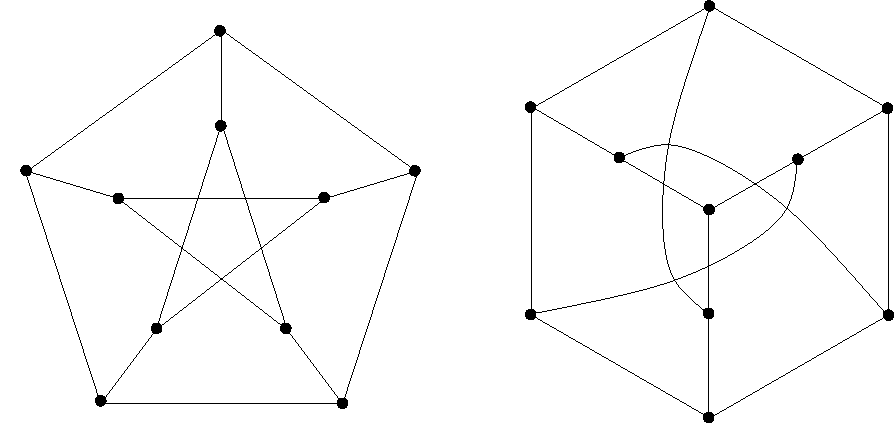
\includegraphics{./petersen_iso.pdf}%
\end{picture}%
\setlength{\unitlength}{3947sp}%
%
\begingroup\makeatletter\ifx\SetFigFont\undefined%
\gdef\SetFigFont#1#2#3#4#5{%
  \reset@font\fontsize{#1}{#2pt}%
  \fontfamily{#3}\fontseries{#4}\fontshape{#5}%
  \selectfont}%
\fi\endgroup%
\begin{picture}(7159,3450)(1453,-8445)
\put(3280,-5177){\makebox(0,0)[lb]{\smash{{\SetFigFont{12}{14.4}{\familydefault}{\mddefault}{\updefault}{\color[rgb]{0,0,0}A}%
}}}}
\put(4846,-6295){\makebox(0,0)[lb]{\smash{{\SetFigFont{12}{14.4}{\familydefault}{\mddefault}{\updefault}{\color[rgb]{0,0,0}B}%
}}}}
\put(4231,-8422){\makebox(0,0)[lb]{\smash{{\SetFigFont{12}{14.4}{\familydefault}{\mddefault}{\updefault}{\color[rgb]{0,0,0}C}%
}}}}
\put(2126,-8430){\makebox(0,0)[lb]{\smash{{\SetFigFont{12}{14.4}{\familydefault}{\mddefault}{\updefault}{\color[rgb]{0,0,0}D}%
}}}}
\put(1468,-6280){\makebox(0,0)[lb]{\smash{{\SetFigFont{12}{14.4}{\familydefault}{\mddefault}{\updefault}{\color[rgb]{0,0,0}E}%
}}}}
\put(3316,-5978){\makebox(0,0)[lb]{\smash{{\SetFigFont{12}{14.4}{\familydefault}{\mddefault}{\updefault}{\color[rgb]{0,0,0}F}%
}}}}
\put(4116,-6756){\makebox(0,0)[lb]{\smash{{\SetFigFont{12}{14.4}{\familydefault}{\mddefault}{\updefault}{\color[rgb]{0,0,0}G}%
}}}}
\put(3839,-7661){\makebox(0,0)[lb]{\smash{{\SetFigFont{12}{14.4}{\familydefault}{\mddefault}{\updefault}{\color[rgb]{0,0,0}H}%
}}}}
\put(2244,-6796){\makebox(0,0)[lb]{\smash{{\SetFigFont{12}{14.4}{\familydefault}{\mddefault}{\updefault}{\color[rgb]{0,0,0}J}%
}}}}
\put(2519,-7663){\makebox(0,0)[lb]{\smash{{\SetFigFont{12}{14.4}{\familydefault}{\mddefault}{\updefault}{\color[rgb]{0,0,0}I}%
}}}}
\end{picture}%


\vspace{.2in}

\item We will use the symbol $\Integers^{\ast}$ to refer to the set of
all integers \emph{except} $0$.  
Define a relation $\relQ$ on the set of all pairs in $\Integers \times \Integers^{\ast}$ (pairs of integers where the second coordinate is non-zero) by
$(a,b) \relQ (c,d) \; \iff \; ad=bc$.  Show that $\relQ$ is an 
equivalence relation.

\item The relation $\relQ$ defined in the previous problem partitions
the set of all pairs of integers into an interesting set of equivalence
classes.  Explain why 

\[ \Rationals \quad = \quad (\Integers \times \Integers^{\ast}) / \relQ. \]

\noindent Ultimately, this is the ``right'' definition of the set 
of rational numbers!

\item Reflect back on the proof in problem 5.  Note that we were fairly
careful in assuring that the second coordinate in the ordered pairs is
non-zero. (This was the whole reason for introducing the 
$\Integers^{\ast}$ notation.)  At what point in the argument did you
use this hypothesis?

\end{enumerate} 

%% Emacs customization
%% 
%% Local Variables: ***
%% TeX-master: "GIAM-hw.tex" ***
%% comment-column:0 ***
%% comment-start: "%% "  ***
%% comment-end:"***" ***
%% End: ***


\newpage

\section{Ordering relations}
%\label{sec:ord_rel}

\noindent{\large \bf Exercises --- \thesection\ }

\begin{enumerate}
\item In population ecology there is a partial order ``predates''
which basically means that one organism feeds upon another.  Strictly
speaking this relation is not transitive; however, if we take the point
of view that when a wolf eats a sheep, it is also eating some of the grass
that the sheep has fed upon, we see that in a certain sense it is transitive.
A chain in this partial order is called a ``food chain'' and so-called 
apex predators are said to ``sit atop the food chain''.  Thus ``apex 
predator'' is a term for a maximal element in this poset.   When poisons
such as mercury and PCBs are introduced into an ecosystem, they tend to
collect disproportionately in the apex predators -- which is why pregnant
women and young children should not eat shark or tuna but sardines 
are fine.

Below is a small example of an ecology partially ordered by ``predates''

\begin{center}
\begin{picture}(0,0)%
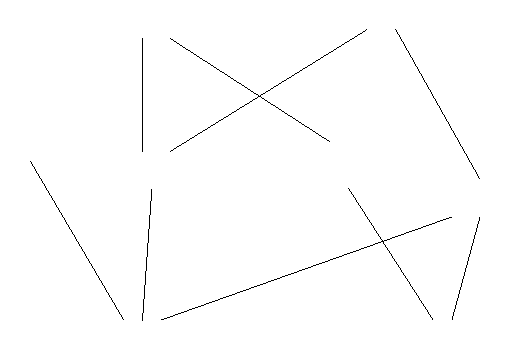
\includegraphics{./ecosystem.pdf}%
\end{picture}%
\setlength{\unitlength}{3947sp}%
%
\begingroup\makeatletter\ifx\SetFigFont\undefined%
\gdef\SetFigFont#1#2#3#4#5{%
  \reset@font\fontsize{#1}{#2pt}%
  \fontfamily{#3}\fontseries{#4}\fontshape{#5}%
  \selectfont}%
\fi\endgroup%
\begin{picture}(4091,2787)(1786,-3376)
\put(2874,-771){\makebox(0,0)[lb]{\smash{{\SetFigFont{12}{14.4}{\rmdefault}{\mddefault}{\updefault}{\color[rgb]{0,0,0}Fox}%
}}}}
\put(4651,-736){\makebox(0,0)[lb]{\smash{{\SetFigFont{12}{14.4}{\rmdefault}{\mddefault}{\updefault}{\color[rgb]{0,0,0}Alligator}%
}}}}
\put(1801,-1786){\makebox(0,0)[lb]{\smash{{\SetFigFont{12}{14.4}{\rmdefault}{\mddefault}{\updefault}{\color[rgb]{0,0,0}Cow}%
}}}}
\put(5401,-2236){\makebox(0,0)[lb]{\smash{{\SetFigFont{12}{14.4}{\rmdefault}{\mddefault}{\updefault}{\color[rgb]{0,0,0}Goose}%
}}}}
\put(2851,-2011){\makebox(0,0)[lb]{\smash{{\SetFigFont{12}{14.4}{\rmdefault}{\mddefault}{\updefault}{\color[rgb]{0,0,0}Duck}%
}}}}
\put(4276,-1936){\makebox(0,0)[lb]{\smash{{\SetFigFont{12}{14.4}{\rmdefault}{\mddefault}{\updefault}{\color[rgb]{0,0,0}Robin}%
}}}}
\put(5101,-3361){\makebox(0,0)[lb]{\smash{{\SetFigFont{12}{14.4}{\rmdefault}{\mddefault}{\updefault}{\color[rgb]{0,0,0}Worms}%
}}}}
\put(2701,-3361){\makebox(0,0)[lb]{\smash{{\SetFigFont{12}{14.4}{\rmdefault}{\mddefault}{\updefault}{\color[rgb]{0,0,0}Grass}%
}}}}
\end{picture}%

\end{center}

Find the largest antichain in this poset.

\newpage

\item Referring to the poset given in exercise 1, match the following.

\begin{tabular}{lr}
\rule{2.3in}{0pt} & \rule{2.3in}{0pt} \\
\begin{minipage}[b]{.4\textwidth}
\begin{enumerate}
\item[1.] An (non-maximal) antichain
\item[2.] A maximal antichain
\item[3.] A maximal element
\item[4.] A (non-maximal) chain
\item[5.] A maximal chain
\item[6.] A cover for ``Worms''
\item[7.] A least element
\item[8.] A minimal element
\end{enumerate}
\end{minipage} 
 & 
\begin{minipage}[b]{.4\textwidth}
\begin{enumerate}
\item[a.] Grass 
\item[b.] Goose
\item[c.] Fox
\item[d.] $\{ \mbox{Grass}, \mbox{Duck} \}$
\item[e.] There isn't one!
\item[f.] $\{ \mbox{Fox}, \mbox{Alligator}, \mbox{Cow} \}$
\item[g.] $\{ \mbox{Cow}, \mbox{Duck}, \mbox{Robin}, \mbox{Goose} \}$
\item[h.] $\{ \mbox{Worms}, \mbox{Robin}, \mbox{Fox} \}$
\end{enumerate} 
\end{minipage} \\
\end{tabular}

\item The graph of the edges of a cube is one in an infinite sequence of 
graphs.  These graphs are defined 
recursively by ``Make two copies of the previous graph then join 
corresponding nodes in the two copies with edges.''  The $0$-dimensional
`cube' is just a single point.  The $1$-dimensional cube is a single edge
with a node at either end.  The $2$-dimensional cube is actually a square
and the $3$-dimensional cube is what we usually mean when we say ``cube.''

\begin{center}
\begin{picture}(0,0)%
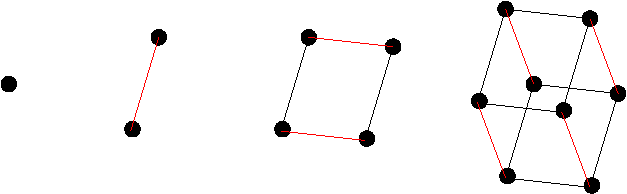
\includegraphics{./0-3_dim_cubes.pdf}%
\end{picture}%
\setlength{\unitlength}{3947sp}%
%
\begingroup\makeatletter\ifx\SetFigFont\undefined%
\gdef\SetFigFont#1#2#3#4#5{%
  \reset@font\fontsize{#1}{#2pt}%
  \fontfamily{#3}\fontseries{#4}\fontshape{#5}%
  \selectfont}%
\fi\endgroup%
\begin{picture}(5015,1548)(1656,-6190)
\end{picture}%

\end{center}

Make a careful drawing of a \index{hypercube}\emph{hypercube} -- which is
the name of the graph that follows the ordinary cube in this sequence.

\item Label the nodes of a hypercube with the divisors of $210$ in order to
produce a Hasse diagram of the poset determined by the divisibility relation.

\item Label the nodes of a hypercube with the subsets of $\{a,b,c,d\}$ 
in order to produce a Hasse diagram of the poset determined by the 
subset containment relation.
  
\item Complete a Hasse diagram for the poset of divisors of 11025 (partially ordered by divisibility).

\item Find a collection of sets so that, when they are partially ordered by $\subseteq$, we obtain the same Hasse diagram as in the previous problem.

\end{enumerate}

%% Emacs customization
%% 
%% Local Variables: ***
%% TeX-master: "GIAM-hw.tex" ***
%% comment-column:0 ***
%% comment-start: "%% "  ***
%% comment-end:"***" ***
%% End: ***


\newpage

\section{Functions}
%\label{sec:functions}


\noindent{\large \bf Exercises --- \thesection\ }


\begin{enumerate}

\item For each of the following functions, give its domain, range and a possible codomain.
  \begin{enumerate}
  \item \wbitemsep $f(x) = \sin{(x)}$
  \item \wbitemsep $g(x) = e^x$
  \item \wbitemsep $h(x) = x^2$
  \item \wbitemsep $m(x) = \frac{x^2+1}{x^2-1}$
  \item \wbitemsep $n(x) = \lfloor x \rfloor$
  \item \wbitemsep $p(x) = \langle \cos{(x)}, \sin{(x)} \rangle $
  \end{enumerate}

\item Find a bijection from the set of odd squares, $\{1, 9, 25, 49, \ldots\}$,
to the non-negative integers, $\Znoneg = \{0,1,2,3, \ldots\}$.
Prove that the function you just determined is both injective and surjective.
Find the inverse function of the bijection above.

\wbvfill

\workbookpagebreak

\item The natural logarithm function $\ln (x)$ is defined by a definite
integral with the variable $x$ in the upper limit.

\[ \ln (x) = \int_{t=1}^{x} \frac{1}{t} \, \mbox{d}t. \]

From this definition we can deduce that $\ln (x)$ is strictly increasing on its
entire domain, $(0, \infty)$.  Why is this true?

We can use the above definition with $x=2$ to find the value of 
$\ln (2) \approx .693$.  We will also take as given the following 
rule (which is valid for all logarithmic functions).

\[ \ln(a^b) = b \ln(a) \]

Use the above information to show that there is neither an upper bound 
nor a lower bound for the values of the natural logarithm.  These facts
together with the information that $\ln$ is strictly increasing show that
$\Rng{\ln} = \Reals$.
 
\wbvfill

\workbookpagebreak

\item Georg Cantor developed a systematic way of listing the rational numbers.
By ``listing'' a set one is actually developing a bijection from $\Naturals$ to
that set.  The method known as ``Cantor's Snake'' creates a bijection from
the naturals to the non-negative rationals.  
First we create an infinite table whose rows
are indexed by positive integers and whose columns are indexed by non-negative
integers -- the entries in this table are rational numbers of the form
``column index'' / ``row index.''  We then follow a snake-like path that
zig-zags across this table -- whenever we encounter a rational number that 
we haven't seen before (in lower terms) we write it down.  This is indicated 
in the diagram below by circling the entries.   

\begin{center}
\begin{picture}(0,0)%
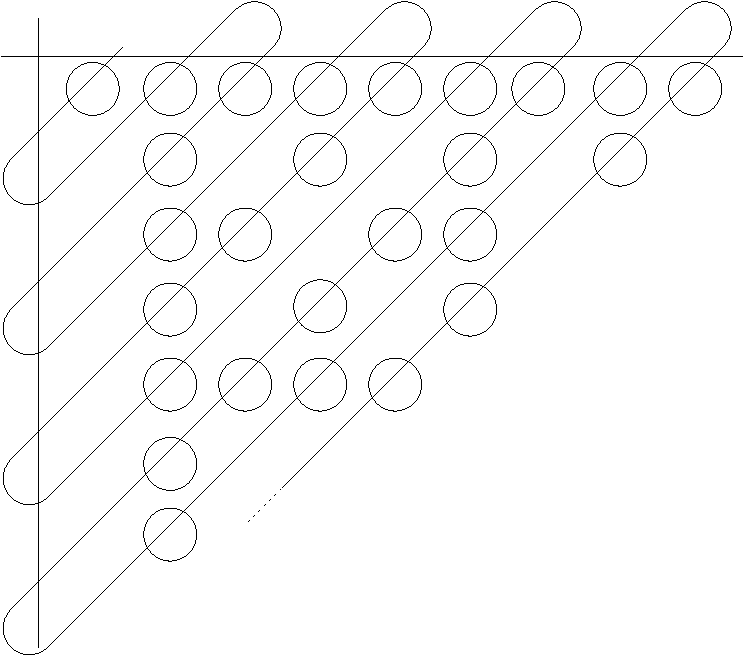
\includegraphics{./Cantor_snake.pdf}%
\end{picture}%
\setlength{\unitlength}{3947sp}%
%
\begingroup\makeatletter\ifx\SetFigFont\undefined%
\gdef\SetFigFont#1#2#3#4#5{%
  \reset@font\fontsize{#1}{#2pt}%
  \fontfamily{#3}\fontseries{#4}\fontshape{#5}%
  \selectfont}%
\fi\endgroup%
\begin{picture}(5949,5243)(1189,-5157)
\put(1801,-286){\makebox(0,0)[lb]{\smash{{\SetFigFont{12}{14.4}{\rmdefault}{\mddefault}{\updefault}{\color[rgb]{0,0,0}0}%
}}}}
\put(2401,-286){\makebox(0,0)[lb]{\smash{{\SetFigFont{12}{14.4}{\rmdefault}{\mddefault}{\updefault}{\color[rgb]{0,0,0}1}%
}}}}
\put(3001,-286){\makebox(0,0)[lb]{\smash{{\SetFigFont{12}{14.4}{\rmdefault}{\mddefault}{\updefault}{\color[rgb]{0,0,0}2}%
}}}}
\put(3601,-286){\makebox(0,0)[lb]{\smash{{\SetFigFont{12}{14.4}{\rmdefault}{\mddefault}{\updefault}{\color[rgb]{0,0,0}3}%
}}}}
\put(4201,-286){\makebox(0,0)[lb]{\smash{{\SetFigFont{12}{14.4}{\rmdefault}{\mddefault}{\updefault}{\color[rgb]{0,0,0}4}%
}}}}
\put(4801,-286){\makebox(0,0)[lb]{\smash{{\SetFigFont{12}{14.4}{\rmdefault}{\mddefault}{\updefault}{\color[rgb]{0,0,0}5}%
}}}}
\put(5401,-286){\makebox(0,0)[lb]{\smash{{\SetFigFont{12}{14.4}{\rmdefault}{\mddefault}{\updefault}{\color[rgb]{0,0,0}6}%
}}}}
\put(6001,-286){\makebox(0,0)[lb]{\smash{{\SetFigFont{12}{14.4}{\rmdefault}{\mddefault}{\updefault}{\color[rgb]{0,0,0}7}%
}}}}
\put(6601,-286){\makebox(0,0)[lb]{\smash{{\SetFigFont{12}{14.4}{\rmdefault}{\mddefault}{\updefault}{\color[rgb]{0,0,0}8}%
}}}}
\put(1351,-661){\makebox(0,0)[lb]{\smash{{\SetFigFont{12}{14.4}{\rmdefault}{\mddefault}{\updefault}{\color[rgb]{0,0,0}1}%
}}}}
\put(1351,-1261){\makebox(0,0)[lb]{\smash{{\SetFigFont{12}{14.4}{\rmdefault}{\mddefault}{\updefault}{\color[rgb]{0,0,0}2}%
}}}}
\put(1351,-1861){\makebox(0,0)[lb]{\smash{{\SetFigFont{12}{14.4}{\rmdefault}{\mddefault}{\updefault}{\color[rgb]{0,0,0}3}%
}}}}
\put(1351,-2461){\makebox(0,0)[lb]{\smash{{\SetFigFont{12}{14.4}{\rmdefault}{\mddefault}{\updefault}{\color[rgb]{0,0,0}4}%
}}}}
\put(1351,-3061){\makebox(0,0)[lb]{\smash{{\SetFigFont{12}{14.4}{\rmdefault}{\mddefault}{\updefault}{\color[rgb]{0,0,0}5}%
}}}}
\put(1351,-3661){\makebox(0,0)[lb]{\smash{{\SetFigFont{12}{14.4}{\rmdefault}{\mddefault}{\updefault}{\color[rgb]{0,0,0}6}%
}}}}
\put(1351,-4261){\makebox(0,0)[lb]{\smash{{\SetFigFont{12}{14.4}{\rmdefault}{\mddefault}{\updefault}{\color[rgb]{0,0,0}7}%
}}}}
\put(1351,-4861){\makebox(0,0)[lb]{\smash{{\SetFigFont{12}{14.4}{\rmdefault}{\mddefault}{\updefault}{\color[rgb]{0,0,0}8}%
}}}}
\put(1801,-661){\makebox(0,0)[lb]{\smash{{\SetFigFont{12}{14.4}{\rmdefault}{\mddefault}{\updefault}{\color[rgb]{0,0,0}0/1}%
}}}}
\put(2401,-661){\makebox(0,0)[lb]{\smash{{\SetFigFont{12}{14.4}{\rmdefault}{\mddefault}{\updefault}{\color[rgb]{0,0,0}1/1}%
}}}}
\put(3001,-661){\makebox(0,0)[lb]{\smash{{\SetFigFont{12}{14.4}{\rmdefault}{\mddefault}{\updefault}{\color[rgb]{0,0,0}2/1}%
}}}}
\put(3601,-661){\makebox(0,0)[lb]{\smash{{\SetFigFont{12}{14.4}{\rmdefault}{\mddefault}{\updefault}{\color[rgb]{0,0,0}3/1}%
}}}}
\put(4201,-661){\makebox(0,0)[lb]{\smash{{\SetFigFont{12}{14.4}{\rmdefault}{\mddefault}{\updefault}{\color[rgb]{0,0,0}4/1}%
}}}}
\put(4801,-661){\makebox(0,0)[lb]{\smash{{\SetFigFont{12}{14.4}{\rmdefault}{\mddefault}{\updefault}{\color[rgb]{0,0,0}5/1}%
}}}}
\put(5401,-661){\makebox(0,0)[lb]{\smash{{\SetFigFont{12}{14.4}{\rmdefault}{\mddefault}{\updefault}{\color[rgb]{0,0,0}6/1}%
}}}}
\put(6001,-661){\makebox(0,0)[lb]{\smash{{\SetFigFont{12}{14.4}{\rmdefault}{\mddefault}{\updefault}{\color[rgb]{0,0,0}7/1}%
}}}}
\put(6601,-661){\makebox(0,0)[lb]{\smash{{\SetFigFont{12}{14.4}{\rmdefault}{\mddefault}{\updefault}{\color[rgb]{0,0,0}8/1}%
}}}}
\put(1801,-1261){\makebox(0,0)[lb]{\smash{{\SetFigFont{12}{14.4}{\rmdefault}{\mddefault}{\updefault}{\color[rgb]{0,0,0}0/2}%
}}}}
\put(2401,-1261){\makebox(0,0)[lb]{\smash{{\SetFigFont{12}{14.4}{\rmdefault}{\mddefault}{\updefault}{\color[rgb]{0,0,0}1/2}%
}}}}
\put(3001,-1261){\makebox(0,0)[lb]{\smash{{\SetFigFont{12}{14.4}{\rmdefault}{\mddefault}{\updefault}{\color[rgb]{0,0,0}2/2}%
}}}}
\put(3601,-1261){\makebox(0,0)[lb]{\smash{{\SetFigFont{12}{14.4}{\rmdefault}{\mddefault}{\updefault}{\color[rgb]{0,0,0}3/2}%
}}}}
\put(4201,-1261){\makebox(0,0)[lb]{\smash{{\SetFigFont{12}{14.4}{\rmdefault}{\mddefault}{\updefault}{\color[rgb]{0,0,0}4/2}%
}}}}
\put(4801,-1261){\makebox(0,0)[lb]{\smash{{\SetFigFont{12}{14.4}{\rmdefault}{\mddefault}{\updefault}{\color[rgb]{0,0,0}5/2}%
}}}}
\put(5401,-1261){\makebox(0,0)[lb]{\smash{{\SetFigFont{12}{14.4}{\rmdefault}{\mddefault}{\updefault}{\color[rgb]{0,0,0}6/2}%
}}}}
\put(6001,-1261){\makebox(0,0)[lb]{\smash{{\SetFigFont{12}{14.4}{\rmdefault}{\mddefault}{\updefault}{\color[rgb]{0,0,0}7/2}%
}}}}
\put(6601,-1261){\makebox(0,0)[lb]{\smash{{\SetFigFont{12}{14.4}{\rmdefault}{\mddefault}{\updefault}{\color[rgb]{0,0,0}8/2}%
}}}}
\put(1801,-1861){\makebox(0,0)[lb]{\smash{{\SetFigFont{12}{14.4}{\rmdefault}{\mddefault}{\updefault}{\color[rgb]{0,0,0}0/3}%
}}}}
\put(2401,-1861){\makebox(0,0)[lb]{\smash{{\SetFigFont{12}{14.4}{\rmdefault}{\mddefault}{\updefault}{\color[rgb]{0,0,0}1/3}%
}}}}
\put(3001,-1861){\makebox(0,0)[lb]{\smash{{\SetFigFont{12}{14.4}{\rmdefault}{\mddefault}{\updefault}{\color[rgb]{0,0,0}2/3}%
}}}}
\put(3601,-1861){\makebox(0,0)[lb]{\smash{{\SetFigFont{12}{14.4}{\rmdefault}{\mddefault}{\updefault}{\color[rgb]{0,0,0}3/3}%
}}}}
\put(4201,-1861){\makebox(0,0)[lb]{\smash{{\SetFigFont{12}{14.4}{\rmdefault}{\mddefault}{\updefault}{\color[rgb]{0,0,0}4/3}%
}}}}
\put(4801,-1861){\makebox(0,0)[lb]{\smash{{\SetFigFont{12}{14.4}{\rmdefault}{\mddefault}{\updefault}{\color[rgb]{0,0,0}5/3}%
}}}}
\put(5401,-1861){\makebox(0,0)[lb]{\smash{{\SetFigFont{12}{14.4}{\rmdefault}{\mddefault}{\updefault}{\color[rgb]{0,0,0}6/3}%
}}}}
\put(6001,-1861){\makebox(0,0)[lb]{\smash{{\SetFigFont{12}{14.4}{\rmdefault}{\mddefault}{\updefault}{\color[rgb]{0,0,0}7/3}%
}}}}
\put(6601,-1861){\makebox(0,0)[lb]{\smash{{\SetFigFont{12}{14.4}{\rmdefault}{\mddefault}{\updefault}{\color[rgb]{0,0,0}8/3}%
}}}}
\put(1801,-2461){\makebox(0,0)[lb]{\smash{{\SetFigFont{12}{14.4}{\rmdefault}{\mddefault}{\updefault}{\color[rgb]{0,0,0}0/4}%
}}}}
\put(2401,-2461){\makebox(0,0)[lb]{\smash{{\SetFigFont{12}{14.4}{\rmdefault}{\mddefault}{\updefault}{\color[rgb]{0,0,0}1/4}%
}}}}
\put(3001,-2461){\makebox(0,0)[lb]{\smash{{\SetFigFont{12}{14.4}{\rmdefault}{\mddefault}{\updefault}{\color[rgb]{0,0,0}2/4}%
}}}}
\put(3601,-2461){\makebox(0,0)[lb]{\smash{{\SetFigFont{12}{14.4}{\rmdefault}{\mddefault}{\updefault}{\color[rgb]{0,0,0}3/4}%
}}}}
\put(4201,-2461){\makebox(0,0)[lb]{\smash{{\SetFigFont{12}{14.4}{\rmdefault}{\mddefault}{\updefault}{\color[rgb]{0,0,0}4/4}%
}}}}
\put(4801,-2461){\makebox(0,0)[lb]{\smash{{\SetFigFont{12}{14.4}{\rmdefault}{\mddefault}{\updefault}{\color[rgb]{0,0,0}5/4}%
}}}}
\put(5401,-2461){\makebox(0,0)[lb]{\smash{{\SetFigFont{12}{14.4}{\rmdefault}{\mddefault}{\updefault}{\color[rgb]{0,0,0}6/4}%
}}}}
\put(6001,-2461){\makebox(0,0)[lb]{\smash{{\SetFigFont{12}{14.4}{\rmdefault}{\mddefault}{\updefault}{\color[rgb]{0,0,0}7/4}%
}}}}
\put(6601,-2461){\makebox(0,0)[lb]{\smash{{\SetFigFont{12}{14.4}{\rmdefault}{\mddefault}{\updefault}{\color[rgb]{0,0,0}8/4}%
}}}}
\put(1801,-3061){\makebox(0,0)[lb]{\smash{{\SetFigFont{12}{14.4}{\rmdefault}{\mddefault}{\updefault}{\color[rgb]{0,0,0}0/5}%
}}}}
\put(2401,-3061){\makebox(0,0)[lb]{\smash{{\SetFigFont{12}{14.4}{\rmdefault}{\mddefault}{\updefault}{\color[rgb]{0,0,0}1/5}%
}}}}
\put(3001,-3061){\makebox(0,0)[lb]{\smash{{\SetFigFont{12}{14.4}{\rmdefault}{\mddefault}{\updefault}{\color[rgb]{0,0,0}2/5}%
}}}}
\put(3601,-3061){\makebox(0,0)[lb]{\smash{{\SetFigFont{12}{14.4}{\rmdefault}{\mddefault}{\updefault}{\color[rgb]{0,0,0}3/5}%
}}}}
\put(4201,-3061){\makebox(0,0)[lb]{\smash{{\SetFigFont{12}{14.4}{\rmdefault}{\mddefault}{\updefault}{\color[rgb]{0,0,0}4/5}%
}}}}
\put(4801,-3061){\makebox(0,0)[lb]{\smash{{\SetFigFont{12}{14.4}{\rmdefault}{\mddefault}{\updefault}{\color[rgb]{0,0,0}5/5}%
}}}}
\put(5401,-3061){\makebox(0,0)[lb]{\smash{{\SetFigFont{12}{14.4}{\rmdefault}{\mddefault}{\updefault}{\color[rgb]{0,0,0}6/5}%
}}}}
\put(6001,-3061){\makebox(0,0)[lb]{\smash{{\SetFigFont{12}{14.4}{\rmdefault}{\mddefault}{\updefault}{\color[rgb]{0,0,0}7/5}%
}}}}
\put(6601,-3061){\makebox(0,0)[lb]{\smash{{\SetFigFont{12}{14.4}{\rmdefault}{\mddefault}{\updefault}{\color[rgb]{0,0,0}8/5}%
}}}}
\put(1801,-3661){\makebox(0,0)[lb]{\smash{{\SetFigFont{12}{14.4}{\rmdefault}{\mddefault}{\updefault}{\color[rgb]{0,0,0}0/6}%
}}}}
\put(2401,-3661){\makebox(0,0)[lb]{\smash{{\SetFigFont{12}{14.4}{\rmdefault}{\mddefault}{\updefault}{\color[rgb]{0,0,0}1/6}%
}}}}
\put(3001,-3661){\makebox(0,0)[lb]{\smash{{\SetFigFont{12}{14.4}{\rmdefault}{\mddefault}{\updefault}{\color[rgb]{0,0,0}2/6}%
}}}}
\put(3601,-3661){\makebox(0,0)[lb]{\smash{{\SetFigFont{12}{14.4}{\rmdefault}{\mddefault}{\updefault}{\color[rgb]{0,0,0}3/6}%
}}}}
\put(4201,-3661){\makebox(0,0)[lb]{\smash{{\SetFigFont{12}{14.4}{\rmdefault}{\mddefault}{\updefault}{\color[rgb]{0,0,0}4/6}%
}}}}
\put(4801,-3661){\makebox(0,0)[lb]{\smash{{\SetFigFont{12}{14.4}{\rmdefault}{\mddefault}{\updefault}{\color[rgb]{0,0,0}5/6}%
}}}}
\put(5401,-3661){\makebox(0,0)[lb]{\smash{{\SetFigFont{12}{14.4}{\rmdefault}{\mddefault}{\updefault}{\color[rgb]{0,0,0}6/6}%
}}}}
\put(6001,-3661){\makebox(0,0)[lb]{\smash{{\SetFigFont{12}{14.4}{\rmdefault}{\mddefault}{\updefault}{\color[rgb]{0,0,0}7/6}%
}}}}
\put(6601,-3661){\makebox(0,0)[lb]{\smash{{\SetFigFont{12}{14.4}{\rmdefault}{\mddefault}{\updefault}{\color[rgb]{0,0,0}8/6}%
}}}}
\put(1801,-4261){\makebox(0,0)[lb]{\smash{{\SetFigFont{12}{14.4}{\rmdefault}{\mddefault}{\updefault}{\color[rgb]{0,0,0}0/7}%
}}}}
\put(2401,-4261){\makebox(0,0)[lb]{\smash{{\SetFigFont{12}{14.4}{\rmdefault}{\mddefault}{\updefault}{\color[rgb]{0,0,0}1/7}%
}}}}
\put(3001,-4261){\makebox(0,0)[lb]{\smash{{\SetFigFont{12}{14.4}{\rmdefault}{\mddefault}{\updefault}{\color[rgb]{0,0,0}2/7}%
}}}}
\put(3601,-4261){\makebox(0,0)[lb]{\smash{{\SetFigFont{12}{14.4}{\rmdefault}{\mddefault}{\updefault}{\color[rgb]{0,0,0}3/7}%
}}}}
\put(4201,-4261){\makebox(0,0)[lb]{\smash{{\SetFigFont{12}{14.4}{\rmdefault}{\mddefault}{\updefault}{\color[rgb]{0,0,0}4/7}%
}}}}
\put(4801,-4261){\makebox(0,0)[lb]{\smash{{\SetFigFont{12}{14.4}{\rmdefault}{\mddefault}{\updefault}{\color[rgb]{0,0,0}5/7}%
}}}}
\put(5401,-4261){\makebox(0,0)[lb]{\smash{{\SetFigFont{12}{14.4}{\rmdefault}{\mddefault}{\updefault}{\color[rgb]{0,0,0}6/7}%
}}}}
\put(6001,-4261){\makebox(0,0)[lb]{\smash{{\SetFigFont{12}{14.4}{\rmdefault}{\mddefault}{\updefault}{\color[rgb]{0,0,0}7/7}%
}}}}
\put(6601,-4261){\makebox(0,0)[lb]{\smash{{\SetFigFont{12}{14.4}{\rmdefault}{\mddefault}{\updefault}{\color[rgb]{0,0,0}8/7}%
}}}}
\put(1801,-4861){\makebox(0,0)[lb]{\smash{{\SetFigFont{12}{14.4}{\rmdefault}{\mddefault}{\updefault}{\color[rgb]{0,0,0}0/8}%
}}}}
\put(2401,-4861){\makebox(0,0)[lb]{\smash{{\SetFigFont{12}{14.4}{\rmdefault}{\mddefault}{\updefault}{\color[rgb]{0,0,0}1/8}%
}}}}
\put(3001,-4861){\makebox(0,0)[lb]{\smash{{\SetFigFont{12}{14.4}{\rmdefault}{\mddefault}{\updefault}{\color[rgb]{0,0,0}2/8}%
}}}}
\put(3601,-4861){\makebox(0,0)[lb]{\smash{{\SetFigFont{12}{14.4}{\rmdefault}{\mddefault}{\updefault}{\color[rgb]{0,0,0}3/8}%
}}}}
\put(4201,-4861){\makebox(0,0)[lb]{\smash{{\SetFigFont{12}{14.4}{\rmdefault}{\mddefault}{\updefault}{\color[rgb]{0,0,0}4/8}%
}}}}
\put(4801,-4861){\makebox(0,0)[lb]{\smash{{\SetFigFont{12}{14.4}{\rmdefault}{\mddefault}{\updefault}{\color[rgb]{0,0,0}5/8}%
}}}}
\put(5401,-4861){\makebox(0,0)[lb]{\smash{{\SetFigFont{12}{14.4}{\rmdefault}{\mddefault}{\updefault}{\color[rgb]{0,0,0}6/8}%
}}}}
\put(6001,-4861){\makebox(0,0)[lb]{\smash{{\SetFigFont{12}{14.4}{\rmdefault}{\mddefault}{\updefault}{\color[rgb]{0,0,0}7/8}%
}}}}
\put(6601,-4861){\makebox(0,0)[lb]{\smash{{\SetFigFont{12}{14.4}{\rmdefault}{\mddefault}{\updefault}{\color[rgb]{0,0,0}8/8}%
}}}}
\end{picture}%

\end{center}

\workbookpagebreak

Effectively this gives us a function $f$ which produces the rational number 
that would be found in a given position in this list.  For example 
$f(1) = 0/1, f(2) = 1/1$ and $f(5) = 1/3$.  

What is $f(26)$?  What is $f(30)$?  What is $f^{-1}(3/4)$? What is $f^{-1}(6/7)$?


  
\wbvfill

\workbookpagebreak
 
\end{enumerate}


%% Emacs customization
%% 
%% Local Variables: ***
%% TeX-master: "GIAM-hw.tex" ***
%% comment-column:0 ***
%% comment-start: "%% "  ***
%% comment-end:"***" ***
%% End: ***


\newpage

\section{Special functions}
%\label{sec:special_functions}

\noindent{\large \bf Exercises --- \thesection\ }

\begin{enumerate}

\item The $n$-th triangular number, denoted $T(n)$, is given by the formula
$T(n) = (n^2 + n)/2$. If we regard this formula as a function from $\Reals$ to
$\Reals$, it fails the horizontal line test and so it is not invertible. Find a
suitable restriction so that T is invertible.

\wbvfill

\item The usual algebraic procedure for inverting $T(x) = (x^2+x)/2$ fails. Use
your knowledge of the geometry of functions and their inverses to find
a formula for the inverse. (Hint: it may be instructive to first invert
the simpler formula $S(x) = x^2/2$ --- this will get you the right vertical
scaling factor.)

\wbvfill

\item What is $\pi_2(W(t))$?  

\wbvfill

\item Find a right inverse for $f(x) = |x|$.

\wbvfill

\workbookpagebreak

\item In three-dimensional space we have projection functions that go onto
the three coordinate axes ($\pi_1$, $\pi_2$ and $\pi_3$) and we also have
projections onto coordinate planes.  For example,
$\pi_{12}: \Reals \times \Reals \times \Reals \longrightarrow \Reals \times \Reals$, defined by

\[ \pi_{12}((x,y,z)) = (x,y) \]

\noindent is the projection onto the $x$--$y$ coordinate plane.

The triple of functions  $(\cos{t}, \sin{t}, t)$ is a parametric
expression for a helix.  Let 
$H = \{ (\cos{t}, \sin{t}, t) \suchthat t \in \Reals \}$ be the set of all
points on the helix.  What is the set $\pi_{12}(H)$ ?  What are the
sets $\pi_{13}(H)$ and $\pi_{23}(H)$?

\wbvfill

\workbookpagebreak

\item Consider the set $\{1, 2, 3, \ldots, 10\}$.  Express the characteristic
function of the subset $S = \{1, 2, 3 \}$ as a set of ordered pairs.

\wbvfill

%\workbookpagebreak

\item If $S$ and $T$ are subsets of a set $D$, what is the product of
their characteristic functions $1_S \cdot 1_T$ ?

\wbvfill

%\workbookpagebreak

\item Evaluate the sum

\[ \sum_{i=1}^{10} \frac{1}{i} \cdot [ i \; \mbox{is prime} ]. \]

\wbvfill

\workbookpagebreak
\end{enumerate}

%% Emacs customization
%% 
%% Local Variables: ***
%% TeX-master: "GIAM-hw.tex" ***
%% comment-column:0 ***
%% comment-start: "%% "  ***
%% comment-end:"***" ***
%% End: ***


%% Emacs customization
%% 
%% Local Variables: ***
%% TeX-master: "GIAM-hw.tex" ***
%% comment-column:0 ***
%% comment-start: "%% "  ***
%% comment-end:"***" ***
%% End: ***


\chapter{Proof techniques III --- Combinatorics}

\section{Counting}
\label{sec:counting}

\begin{enumerate}
\item Determine the number of entries in the following sequences.

  \begin{enumerate}
  \item \wbitemsep $(999, 1000, 1001, \ldots  2006)$
  \item \wbitemsep $(13, 15, 17, \ldots 199)$
  \item \wbitemsep $(13, 19, 25, \ldots 601)$
  \item \wbitemsep $(5, 10, 17, 26, 37, \ldots 122)$
  \item \wbitemsep $(27, 64, 125, 216, \ldots 8000)$
  \item \wbitemsep $(7, 11, 19, 35, 67, \ldots 131075)$
  \end{enumerate}

\workbookpagebreak

\item How many ``full houses'' are there in Yahtzee?  (A full house is a pair
together with a three-of-a-kind.)

\wbvfill

\item In how many ways can you get ``two pairs'' in Yahtzee?

\wbvfill

\item Prove that the binomial coefficients $\displaystyle \binom{n+k-1}{k}$
and $\displaystyle \binom{n+k-1}{n-1}$ are equal.

\wbvfill

\workbookpagebreak

\item The ``Cryptographer's alphabet'' is used to supply small examples
in coding and cryptography.  It consists of the first 6 letters, $\{a, b, c, d, e, f\}$.  How many ``words'' of length up to 6 can be made with this 
alphabet?  (A word need not actually be a word in English, for example 
both ``fed'' and ``dfe'' would be words in the sense we are using the term.)

\wbvfill

\item How many ``words'' are there of length 4, with distinct letters from the 
Cryptographer's alphabet, in which the letters appear in increasing order 
alphabetically?  (``Acef'' would be one such word, but ``cafe'' would not.)

\wbvfill

\item How many ``words'' are there of length 4 from the 
Cryptographer's alphabet, with repeated letters allowed,
 in which the letters appear in non-decreasing order alphabetically?

\wbvfill

\workbookpagebreak

\item How many subsets does a finite set have?

\wbvfill

\item How many handshakes will transpire when $n$ people first meet?

\wbvfill

\item How many functions are there from a set of size $n$ to a set of size $m$?

\wbvfill

\item How many relations are there from a set of size $n$ to a set of size $m$?

\wbvfill

\workbookpagebreak

\end{enumerate}

%% Emacs customization
%% 
%% Local Variables: ***
%% TeX-master: "GIAM-hw.tex" ***
%% comment-column:0 ***
%% comment-start: "%% "  ***
%% comment-end:"***" ***
%% End: ***



\clearpage

\section{Parity and Counting arguments}

\noindent{\large \bf Exercises --- \thesection\ }


\begin{enumerate}

\item A walking tour of K\"{o}nigsberg such as is described in this section,
or more generally, a circuit through an arbitrary graph that crosses each
edge precisely once and begins and ends at the same node is known as
an \index{Eulerian circuit} \emph{Eulerian circuit}.  An \index{Eulerian
path} \emph{Eulerian path} also crosses every edge of a graph exactly
once but it begins and ends at distinct nodes.  For each of the following
graphs determine whether an Eulerian circuit or path is possible, and if so,
draw it.

\begin{center}
\begin{picture}(0,0)%
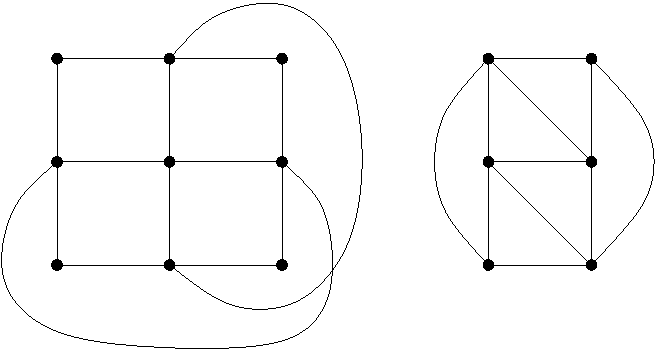
\includegraphics{./Euler_circuit_problems_a.pdf}%
\end{picture}%
\setlength{\unitlength}{3947sp}%
%
\begingroup\makeatletter\ifx\SetFigFont\undefined%
\gdef\SetFigFont#1#2#3#4#5{%
  \reset@font\fontsize{#1}{#2pt}%
  \fontfamily{#3}\fontseries{#4}\fontshape{#5}%
  \selectfont}%
\fi\endgroup%
\begin{picture}(5244,2786)(745,-2541)
\end{picture}%

\end{center}

\begin{center}
\begin{picture}(0,0)%
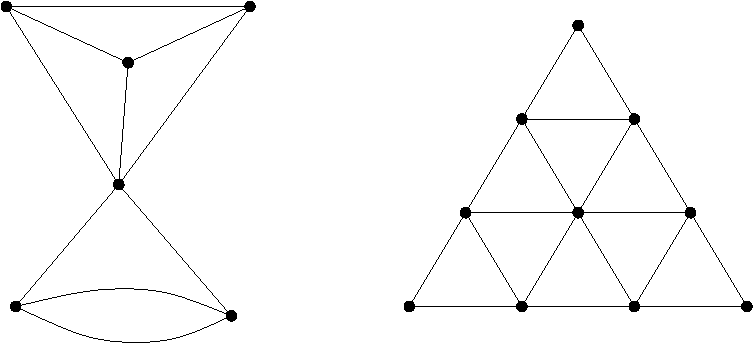
\includegraphics{./Euler_circuit_problems_b.pdf}%
\end{picture}%
\setlength{\unitlength}{3947sp}%
%
\begingroup\makeatletter\ifx\SetFigFont\undefined%
\gdef\SetFigFont#1#2#3#4#5{%
  \reset@font\fontsize{#1}{#2pt}%
  \fontfamily{#3}\fontseries{#4}\fontshape{#5}%
  \selectfont}%
\fi\endgroup%
\begin{picture}(6025,2749)(1226,-3136)
\end{picture}%

\end{center}

\item Complete the proof of the fact that ``Every graph has an even number
of odd nodes.''

\wbvfill

\item Provide an argument as to why an $8 \times 8$ chessboard with 
two squares pruned from diagonally opposite corners cannot be tiled
with dominoes.

\wbvfill

\workbookpagebreak

\item Prove that, if $n$ is odd, any $n \times n$ chessboard with 
a square the same color as one of its corners pruned can be tiled by
dominoes.

\wbvfill

\item The five \index{tetromino} tetrominoes (familiar to players of the video game
Tetris) are relatives of dominoes made up of four small squares.

\begin{center}
\begin{picture}(0,0)%
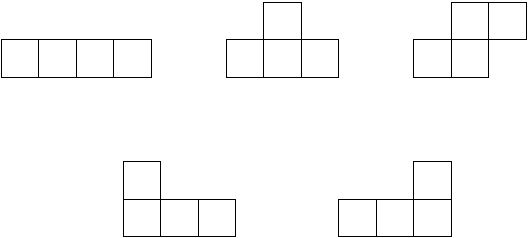
\includegraphics{figures/five_tetrominoes.pdf}%
\end{picture}%
\setlength{\unitlength}{3947sp}%
%
\begingroup\makeatletter\ifx\SetFigFont\undefined%
\gdef\SetFigFont#1#2#3#4#5{%
  \reset@font\fontsize{#1}{#2pt}%
  \fontfamily{#3}\fontseries{#4}\fontshape{#5}%
  \selectfont}%
\fi\endgroup%
\begin{picture}(4224,1899)(1189,-1948)
\end{picture}%

\end{center}

\noindent All together these five tetrominoes contain 20 squares
so it is conceivable that they could be used to tile a $4 \times 5$
chessboard.  Prove that this is actually impossible.

\wbvfill

\workbookpagebreak

\item State necessary and sufficient conditions for the existence of
an Eulerian circuit in a graph.  

\wbvfill

\item  State necessary and sufficient conditions for the existence of
an Eulerian path in a graph.  

\wbvfill

\newpage

\item Construct magic squares of order 4 and 5.

\wbvfill

\workbookpagebreak

\item A magic hexagon of order 2 would consist of filling-in
the numbers from 1 to 7 in the hexagonal array below.  The magic
condition means that each of the 9 ``lines'' of adjacent hexagons
would have the same sum.  Is this possible?

\begin{center}
\begin{picture}(0,0)%
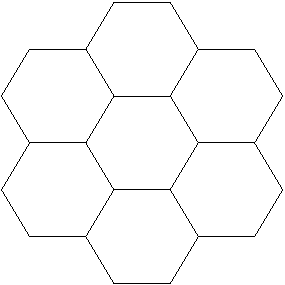
\includegraphics{figures/magic_hexagon.pdf}%
\end{picture}%
\setlength{\unitlength}{3947sp}%
%
\begingroup\makeatletter\ifx\SetFigFont\undefined%
\gdef\SetFigFont#1#2#3#4#5{%
  \reset@font\fontsize{#1}{#2pt}%
  \fontfamily{#3}\fontseries{#4}\fontshape{#5}%
  \selectfont}%
\fi\endgroup%
\begin{picture}(2274,2274)(2164,-3073)
\end{picture}%

\end{center}

\wbvfill

\item Is there a magic hexagon of order 3?

\wbvfill

\end{enumerate}



%% Emacs customization
%% 
%% Local Variables: ***
%% TeX-master: "GIAM-hw.tex" ***
%% comment-column:0 ***
%% comment-start: "%% "  ***
%% comment-end:"***" ***
%% End: ***



\clearpage


\section{The pigeonhole principle}

\noindent{\large \bf Exercises --- \thesection\ }

\begin{enumerate}

\item The statement that there are two non-bald New Yorkers with
the same number of hairs on their heads requires some careful 
estimates to justify it.  Please justify it.

\wbvfill

\item A mathematician, who always rises earlier than her spouse, has
developed a scheme -- using the pigeonhole principle -- to ensure that
she always has a matching pair of socks.  She keeps only blue socks, green 
socks and
black socks in her sock drawer -- 10 of each.  So as not to wake her 
husband she must
select some number of socks from her drawer in the early morning dark
and take them with her to the adjacent bathroom where she dresses.
What number of socks does she choose?

\wbvfill

\workbookpagebreak

\item If we select $1001$ numbers from the set $\{1, 2, 3, \ldots, 2000\}$
it is certain that there will be two numbers selected such that one divides
the other.  We can prove this fact by noting that every number in the given
set can be expressed in the form $2^k \cdot m$ where $m$ is an odd number
and using the pigeonhole principle.  Write-up this proof.

\wbvfill

\item Given any set of $53$ integers, show that there are two of them
having the property 
that either their sum or their difference is evenly divisible by $103$.

\wbvfill

\workbookpagebreak

\item Prove that if $10$ points are placed inside a square of side length 3,
there will be 2 points within $\sqrt{2}$ of one another.

\wbvfill

\item Prove that if $10$ points are placed inside an equilateral triangle
of side length 3, there will be 2 points within $1$ of one another.

\wbvfill

\workbookpagebreak

\item Prove that in a simple graph (an undirected graph with no 
loops or parallel edges) having $n$ nodes, there must be two nodes 
having the same degree. 

\wbvfill

\workbookpagebreak

\end{enumerate}


%% Emacs customization
%% 
%% Local Variables: ***
%% TeX-master: "GIAM-hw.tex" ***
%% comment-column:0 ***
%% comment-start: "%% "  ***
%% comment-end:"***" ***
%% End: ***



\clearpage

\section{The algebra of combinations}

\noindent{\large \bf Exercises --- \thesection\ }

\begin{enumerate}

\item Use the binomial theorem (with $x=1000$ and $y=1$) to calculate
$1001^6$.

\wbvfill

\item Find $(2x+3)^5$.

\wbvfill

\item Find $(x^2+y^2)^6$.

\wbvfill

\workbookpagebreak

\item The following diagram contains a 3-dimensional analog of
Pascal's triangle that we might call ``Pascal's tetrahedron.'' 
What would the next layer look like?

\begin{center}
\begin{picture}(0,0)%
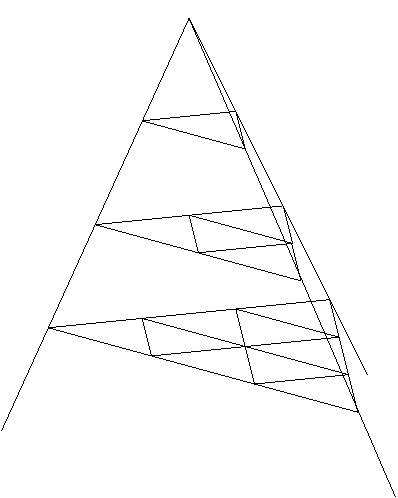
\includegraphics{figures/Pascals_tetrahedron.pdf}%
\end{picture}%
\setlength{\unitlength}{3947sp}%
%
\begingroup\makeatletter\ifx\SetFigFont\undefined%
\gdef\SetFigFont#1#2#3#4#5{%
  \reset@font\fontsize{#1}{#2pt}%
  \fontfamily{#3}\fontseries{#4}\fontshape{#5}%
  \selectfont}%
\fi\endgroup%
\begin{picture}(3174,3971)(3889,-4123)
\put(4876,-1111){\makebox(0,0)[lb]{\smash{{\SetFigFont{12}{14.4}{\familydefault}{\mddefault}{\updefault}{\color[rgb]{0,0,0}$1$}%
}}}}
\put(5851,-1036){\makebox(0,0)[lb]{\smash{{\SetFigFont{12}{14.4}{\familydefault}{\mddefault}{\updefault}{\color[rgb]{0,0,0}$1$}%
}}}}
\put(5926,-1411){\makebox(0,0)[lb]{\smash{{\SetFigFont{12}{14.4}{\familydefault}{\mddefault}{\updefault}{\color[rgb]{0,0,0}$1$}%
}}}}
\put(6526,-2536){\makebox(0,0)[lb]{\smash{{\SetFigFont{12}{14.4}{\familydefault}{\mddefault}{\updefault}{\color[rgb]{0,0,0}$1$}%
}}}}
\put(6226,-1786){\makebox(0,0)[lb]{\smash{{\SetFigFont{12}{14.4}{\familydefault}{\mddefault}{\updefault}{\color[rgb]{0,0,0}$1$}%
}}}}
\put(4501,-1936){\makebox(0,0)[lb]{\smash{{\SetFigFont{12}{14.4}{\familydefault}{\mddefault}{\updefault}{\color[rgb]{0,0,0}$1$}%
}}}}
\put(4135,-2779){\makebox(0,0)[lb]{\smash{{\SetFigFont{12}{14.4}{\familydefault}{\mddefault}{\updefault}{\color[rgb]{0,0,0}$1$}%
}}}}
\put(4955,-2642){\makebox(0,0)[lb]{\smash{{\SetFigFont{12}{14.4}{\familydefault}{\mddefault}{\updefault}{\color[rgb]{0,0,0}$3$}%
}}}}
\put(5719,-2580){\makebox(0,0)[lb]{\smash{{\SetFigFont{12}{14.4}{\familydefault}{\mddefault}{\updefault}{\color[rgb]{0,0,0}$3$}%
}}}}
\put(6631,-2841){\makebox(0,0)[lb]{\smash{{\SetFigFont{12}{14.4}{\familydefault}{\mddefault}{\updefault}{\color[rgb]{0,0,0}$3$}%
}}}}
\put(6720,-3140){\makebox(0,0)[lb]{\smash{{\SetFigFont{12}{14.4}{\familydefault}{\mddefault}{\updefault}{\color[rgb]{0,0,0}$3$}%
}}}}
\put(6782,-3494){\makebox(0,0)[lb]{\smash{{\SetFigFont{12}{14.4}{\familydefault}{\mddefault}{\updefault}{\color[rgb]{0,0,0}$1$}%
}}}}
\put(5861,-3409){\makebox(0,0)[lb]{\smash{{\SetFigFont{12}{14.4}{\familydefault}{\mddefault}{\updefault}{\color[rgb]{0,0,0}$3$}%
}}}}
\put(5026,-3184){\makebox(0,0)[lb]{\smash{{\SetFigFont{12}{14.4}{\familydefault}{\mddefault}{\updefault}{\color[rgb]{0,0,0}$3$}%
}}}}
\put(5866,-2894){\makebox(0,0)[lb]{\smash{{\SetFigFont{12}{14.4}{\familydefault}{\mddefault}{\updefault}{\color[rgb]{0,0,0}$6$}%
}}}}
\put(6319,-2377){\makebox(0,0)[lb]{\smash{{\SetFigFont{12}{14.4}{\familydefault}{\mddefault}{\updefault}{\color[rgb]{0,0,0}$1$}%
}}}}
\put(6271,-2102){\makebox(0,0)[lb]{\smash{{\SetFigFont{12}{14.4}{\familydefault}{\mddefault}{\updefault}{\color[rgb]{0,0,0}$2$}%
}}}}
\put(5330,-1817){\makebox(0,0)[lb]{\smash{{\SetFigFont{12}{14.4}{\familydefault}{\mddefault}{\updefault}{\color[rgb]{0,0,0}$2$}%
}}}}
\put(5406,-2329){\makebox(0,0)[lb]{\smash{{\SetFigFont{12}{14.4}{\familydefault}{\mddefault}{\updefault}{\color[rgb]{0,0,0}$2$}%
}}}}
\put(5441,-299){\makebox(0,0)[lb]{\smash{{\SetFigFont{12}{14.4}{\familydefault}{\mddefault}{\updefault}{\color[rgb]{0,0,0}$1$}%
}}}}
\end{picture}%

\end{center}

\wbvfill

\item The student government at Lagrange High consists of 24 members chosen
from amongst the general student body of 210. Additionally, there
is a steering committee of 5 members chosen from amongst those in
student government. Use the multiplication rule to determine two different
formulas for the total number of possible governance structures.

\wbvfill

\workbookpagebreak

\item Prove the identity
\[ \binom{n}{k} \cdot \binom{k}{r} \; = \; \binom{n}{r} \cdot \binom{n-r}{k-r} \]
combinatorially.

\wbvfill

\item Prove the binomial theorem.

\[ \forall n \in \Naturals, \; \forall x,y \in \Reals, \; 
(x+y)^n \; = \; \sum_{k=0}^n \binom{n}{k} x^{n-k}y^k \]

\wbvfill

\workbookpagebreak

\end{enumerate}

%% Emacs customization
%% 
%% Local Variables: ***
%% TeX-master: "GIAM-hw.tex" ***
%% comment-column:0 ***
%% comment-start: "%% "  ***
%% comment-end:"***" ***
%% End: ***




%% Emacs customization
%% 
%% Local Variables: ***
%% TeX-master: "GIAM-hw.tex" ***
%% comment-column:0 ***
%% comment-start: "%% "  ***
%% comment-end:"***" ***
%% End: ***


\chapter{Cardinality}
%\label{ch:card}


\section{Equivalent sets}
%\label{sec:equiv_sets}

\noindent{\large \bf Exercises --- \thesection\ }

\begin{enumerate}
\item Name four sets in the equivalence class of $\{1, 2, 3\}$.
\item Prove that set equivalence is an equivalence relation.
\item Construct a Venn diagram showing the relationships between the sets of
sets which are finite, infinite, countable, denumerable and uncountable.
\item Place the sets $\Naturals$, $\Reals$, $\Rationals$, $\Integers$, $\Integers \times \Integers$, $\Complexes$, $\Naturals_{2007}$ and $\emptyset$; 
somewhere on the Venn diagram above. (Note to students (and graders): 
there are no wrong answers to this question, the point is to see what 
your intuition about these sets says at this point.)
\end{enumerate}
 
%% Emacs customization
%% 
%% Local Variables: ***
%% TeX-master: "GIAM-hw.tex" ***
%% comment-column:0 ***
%% comment-start: "%% "  ***
%% comment-end:"***" ***
%% End: ***



\newpage

\section{Examples of set equivalence}

\noindent{\large \bf Exercises --- \thesection\ }

\begin{enumerate}
\item  Prove that positive numbers of the form $3k +1$ are equinumerous with
positive numbers of the form $4k + 2$.

\wbvfill

\item Prove that $\displaystyle f(x) =  c + \frac{(x-a)(d-c)}{(b-a)}$ 
provides a bijection from the interval $[a, b]$ to the interval $[c, d]$.

\wbvfill

\workbookpagebreak

\item Prove that any two circles are equinumerous (as sets of points).

\wbvfill

\item Determine a formula for the bijection from $(-1, 1)$ to the line $y = 1$
determined by vertical projection onto the upper half of the unit circle,
followed by projection from the point $(0, 0)$.

\wbvfill

\workbookpagebreak

\item  It is possible to generalize the argument that shows a line segment is
equivalent to a line to higher dimensions.   In two dimensions we would
show that the unit disk (the interior of the unit circle) is equinumerous
with the entire plane $\Reals \times \Reals$.   In three dimensions we would show that
the unit ball (the interior of the unit sphere) is equinumerous with the
entire space $\Reals^3 = \Reals \times \Reals \times \Reals$.  Here we 
would like you to prove the two-dimensional case.

Gnomonic projection is a style of map rendering in which a portion of a
sphere is projected onto a plane that is tangent to the sphere.  The 
sphere's center is used as the point to project from.  Combine 
vertical projection from the unit disk
in the x--y plane to the upper half of the unit sphere $x^2 + y^2 + z^2 = 1$,
with gnomonic projection from the unit sphere to the plane z = 1, to
deduce a bijection between the unit disk and the (infinite) plane.

\wbvfill

\end{enumerate}
 
%% Emacs customization
%% 
%% Local Variables: ***
%% TeX-master: "GIAM-hw.tex" ***
%% comment-column:0 ***
%% comment-start: "%% "  ***
%% comment-end:"***" ***
%% End: ***



\newpage

\section{Cantor's theorem}
%\label{sec:cantors_thm}

\noindent{\large \bf Exercises --- \thesection\ }

\begin{enumerate}
\item Determine a substitution rule -- a consistent way of replacing one digit
with another along the diagonal so that a diagonalization proof showing
that the interval (0, 1) is uncountable will work in decimal. Write up
the proof.

\wbvfill

\item Can a diagonalization proof showing that the interval (0, 1) is uncountable
be made workable in base-3 (ternary) notation?

\wbvfill

\workbookpagebreak

\item In the proof of Cantor's theorem we construct a set $S$ that cannot
be in the image of a presumed bijection from $A$ to ${\mathcal P}(A)$.  
Suppose $A = \{1, 2, 3\}$ and f determines the following correspondences: 
$1 \longleftrightarrow \emptyset$,
$2 \longleftrightarrow \{1, 3\}$ and $3 \longleftrightarrow \{1, 2, 3\}$. 
What is $S$?

\wbvfill

\item An argument very similar to the one embodied in the proof of Cantor's
theorem is found in the Barber's paradox. This paradox was
originally introduced in the popular press in order to give laypeople an
understanding of Cantor's theorem and Russell's paradox. It sounds
somewhat sexist to modern ears. (For example, it is presumed without
comment that the Barber is male.)

\begin{quote}
In a small town there is a Barber who shaves those men (and
only those men) who do not shave themselves. Who shaves
the Barber?
\end{quote}

Explain the similarity to the proof of Cantor's theorem.

\wbvfill

\workbookpagebreak

\item Cantor's theorem, applied to the set of all sets leads to an interesting
paradox. The power set of the set of all sets is a collection of sets, so
it must be contained in the set of all sets. Discuss the paradox and
determine a way of resolving it.

\wbvfill

\item Verify that the final deduction in the proof of Cantor's theorem, 
``$(y \in S  \implies  y \notin S) \land  (y \notin S \implies y \in S)$,'' 
is truly a contradiction.

\wbvfill

\workbookpagebreak

\end{enumerate}

%% Emacs customization
%% 
%% Local Variables: ***
%% TeX-master: "GIAM-hw.tex" ***
%% comment-column:0 ***
%% comment-start: "%% "  ***
%% comment-end:"***" ***
%% End: ***



\newpage

\section{Dominance}

\noindent{\large \bf Exercises --- \thesection\ }

\begin{enumerate}
\item How could the clerk at the Hilbert Hotel accommodate a countable
number of new guests?

\wbvfill

\item Let $F$ be the collection of all real-valued functions 
defined on the real line.  Find an injection from $\Reals$ to $F$.  Do you 
think it is possible to find an injection going the other way?  In 
other words, do you think that $F$ and $\Reals$ are equivalent?  Explain.

\wbvfill

\workbookpagebreak

\item Fill in the details of the proof that dominance is an ordering relation.
(You may simply cite the C-B-S theorem in proving anti-symmetry.)

\wbvfill

\item We can inject $\Rationals$ into $\Integers$ by sending 
$\displaystyle \pm \frac{a}{b}$ to $\displaystyle \pm 2^a3^b$.  
 Use this and another obvious injection to (in light of the C-B-S 
theorem) reaffirm the equivalence of these sets.

\wbvfill

\end{enumerate}

%% Emacs customization
%% 
%% Local Variables: ***
%% TeX-master: "GIAM-hw.tex" ***
%% comment-column:0 ***
%% comment-start: "%% "  ***
%% comment-end:"***" ***
%% End: ***



%\newpage

%\section[CH and GCH]{The continuum hypothesis and the generalized continuum hypothesis}

%
No Exercises in this section.
 
%% Emacs customization
%% 
%% Local Variables: ***
%% TeX-master: "GIAM-hw.tex" ***
%% comment-column:0 ***
%% comment-start: "%% "  ***
%% comment-end:"***" ***
%% End: ***


 
%% Emacs customization
%% 
%% Local Variables: ***
%% TeX-master: "GIAM-hw.tex" ***
%% comment-column:0 ***
%% comment-start: "%% "  ***
%% comment-end:"***" ***
%% End: ***


\chapter{Proof techniques IV --- Magic}

\section{Morley's miracle}

\noindent{\large \bf Exercises --- \thesection\ }

\begin{enumerate}
\item What value should we get if we sum all of the
angles that appear around one of the interior vertices in the 
finished diagram?  Verify that all three have the correct sum.

\begin{center}
\begin{picture}(0,0)%
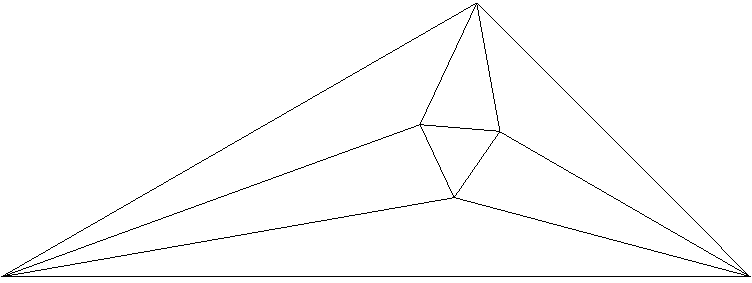
\includegraphics{figures/Morley_finished.pdf}%
\end{picture}%
\setlength{\unitlength}{3947sp}%
%
\begingroup\makeatletter\ifx\SetFigFont\undefined%
\gdef\SetFigFont#1#2#3#4#5{%
  \reset@font\fontsize{#1}{#2pt}%
  \fontfamily{#3}\fontseries{#4}\fontshape{#5}%
  \selectfont}%
\fi\endgroup%
\begin{picture}(6013,2252)(1191,-3877)
\put(1877,-3530){\makebox(0,0)[lb]{\smash{{\SetFigFont{12}{14.4}{\familydefault}{\mddefault}{\updefault}{\color[rgb]{0,0,0}$a$}%
}}}}
\put(2009,-3808){\makebox(0,0)[lb]{\smash{{\SetFigFont{12}{14.4}{\familydefault}{\mddefault}{\updefault}{\color[rgb]{0,0,0}$a$}%
}}}}
\put(1942,-3654){\makebox(0,0)[lb]{\smash{{\SetFigFont{12}{14.4}{\familydefault}{\mddefault}{\updefault}{\color[rgb]{0,0,0}$a$}%
}}}}
\put(4595,-3190){\makebox(0,0)[lb]{\smash{{\SetFigFont{12}{14.4}{\familydefault}{\mddefault}{\updefault}{\color[rgb]{0,0,0}$b^{\star}$}%
}}}}
\put(4392,-2806){\makebox(0,0)[lb]{\smash{{\SetFigFont{12}{14.4}{\familydefault}{\mddefault}{\updefault}{\color[rgb]{0,0,0}$c^{\star}$}%
}}}}
\put(4253,-2611){\makebox(0,0)[lb]{\smash{{\SetFigFont{12}{14.4}{\familydefault}{\mddefault}{\updefault}{\color[rgb]{0,0,0}$b^{\star\star}$}%
}}}}
\put(4723,-1915){\makebox(0,0)[lb]{\smash{{\SetFigFont{12}{14.4}{\familydefault}{\mddefault}{\updefault}{\color[rgb]{0,0,0}$c$}%
}}}}
\put(5094,-1936){\makebox(0,0)[lb]{\smash{{\SetFigFont{12}{14.4}{\familydefault}{\mddefault}{\updefault}{\color[rgb]{0,0,0}$c$}%
}}}}
\put(4919,-1942){\makebox(0,0)[lb]{\smash{{\SetFigFont{12}{14.4}{\familydefault}{\mddefault}{\updefault}{\color[rgb]{0,0,0}$c$}%
}}}}
\put(4683,-3383){\makebox(0,0)[lb]{\smash{{\SetFigFont{12}{14.4}{\familydefault}{\mddefault}{\updefault}{\color[rgb]{0,0,0}$c^{\star\star}$}%
}}}}
\put(6478,-3804){\makebox(0,0)[lb]{\smash{{\SetFigFont{12}{14.4}{\familydefault}{\mddefault}{\updefault}{\color[rgb]{0,0,0}$b$}%
}}}}
\put(6509,-3633){\makebox(0,0)[lb]{\smash{{\SetFigFont{12}{14.4}{\familydefault}{\mddefault}{\updefault}{\color[rgb]{0,0,0}$b$}%
}}}}
\put(6570,-3475){\makebox(0,0)[lb]{\smash{{\SetFigFont{12}{14.4}{\familydefault}{\mddefault}{\updefault}{\color[rgb]{0,0,0}$b$}%
}}}}
\put(4610,-2604){\makebox(0,0)[lb]{\smash{{\SetFigFont{12}{14.4}{\familydefault}{\mddefault}{\updefault}{\color[rgb]{0,0,0}$a^{\star}$}%
}}}}
\put(4986,-2628){\makebox(0,0)[lb]{\smash{{\SetFigFont{12}{14.4}{\familydefault}{\mddefault}{\updefault}{\color[rgb]{0,0,0}$b^{\star}$}%
}}}}
\put(5221,-2672){\makebox(0,0)[lb]{\smash{{\SetFigFont{12}{14.4}{\familydefault}{\mddefault}{\updefault}{\color[rgb]{0,0,0}$a^{\star\star}$}%
}}}}
\put(5135,-2863){\makebox(0,0)[lb]{\smash{{\SetFigFont{12}{14.4}{\familydefault}{\mddefault}{\updefault}{\color[rgb]{0,0,0}$c^{\star}$}%
}}}}
\put(4902,-3203){\makebox(0,0)[lb]{\smash{{\SetFigFont{12}{14.4}{\familydefault}{\mddefault}{\updefault}{\color[rgb]{0,0,0}$a^{\star}$}%
}}}}
\end{picture}%

\end{center}

\item In this section we talked about similarity.  Two figures in 
the plane are 
similar if it is possible to turn one into the other
by a sequence of mappings: a translation, a rotation and a scaling.  

Geometric similarity is an equivalence relation.  To fix our
notation, let $T(x,y)$ represent a generic translation, $R(x,y)$ a rotation
and $S(x,y)$ a scaling -- thus a generic similarity is a function from
$\Reals^2$ to $\Reals^2$ that can be written in the form $S(R(T(x,y)))$.

Discuss the three properties of an equivalence relation (reflexivity, symmetry and transitivity) in terms of geometric similarity.

\end{enumerate}

%% Emacs customization
%% 
%% Local Variables: ***
%% TeX-master: "GIAM-hw.tex" ***
%% comment-column:0 ***
%% comment-start: "%% "  ***
%% comment-end:"***" ***
%% End: ***



\newpage

\section{Five steps into the void}

\noindent{\large \bf Exercises --- \thesection\ }

\begin{enumerate}
\item Do the algebra (and show all your work!) to prove that invariant
defined in this section actually has the value 1 for the set of all the
men occupying the $x$-axis and the lower half-plane.

\wbvfill

\workbookpagebreak

\item ``Escape of the clones'' is a  nice puzzle, originally proposed by Maxim Kontsevich.  The game
is played on an infinite checkerboard restricted to the first quadrant -- that is the squares may be 
identified with points having integer coordinates $(x,y)$ with $x>0$ and $y>0$.  The ``clones'' are markers
(checkers, coins, small rocks, whatever\ldots) that can move in only one fashion -- if the squares immediately
above and to the right of a clone are empty, then it can make a ``clone move.''   The clone moves one space
up and a copy is placed in the cell one to the right.  We begin with three clones occupying cells $(1,1), (2,1)$ and $(1,2)$ -- we'll refer to those three checkerboard squares as ``the prison.''  The question is this:  can these
three clones escape the prison?

You must either demonstrate a sequence of moves that frees all three clones or provide an argument that the task is impossible.

\wbvfill

\end{enumerate}

%% Emacs customization
%% 
%% Local Variables: ***
%% TeX-master: "GIAM-hw.tex" ***
%% comment-column:0 ***
%% comment-start: "%% "  ***
%% comment-end:"***" ***
%% End: ***



\newpage

\section{Monge's circle theorem}

\noindent{\large \bf Exercises --- \thesection\ }

\begin{enumerate}
\item There is a scenario where the proof we have sketched for
Monge's circle theorem doesn't really work.  Can you envision it?
Hint: consider two relatively large spheres and one that is quite
small.
\end{enumerate}



%% Emacs customization
%% 
%% Local Variables: ***
%% TeX-master: "GIAM-hw.tex" ***
%% comment-column:0 ***
%% comment-start: "%% "  ***
%% comment-end:"***" ***
%% End: ***



%% Emacs customization
%% 
%% Local Variables: ***
%% TeX-master: "GIAM-hw.tex" ***
%% comment-column:0 ***
%% comment-start: "%% "  ***
%% comment-end:"***" ***
%% End: ***




\end{document}

